\documentclass[dvipsnames]{article}

\usepackage[final]{slm}
\usepackage[utf8]{inputenc} % allow utf-8 input
\usepackage[T1]{fontenc}    % use 8-bit T1 fonts
\usepackage{url}            % simple URL typesetting
\usepackage{booktabs}       % professional-quality tables
\usepackage{amsfonts}       % blackboard math symbols
\usepackage{nicefrac}       % compact symbols for 1/2, etc.
\usepackage{booktabs} 
\usepackage{multirow}
\usepackage{wrapfig}
\usepackage{amssymb}
\usepackage{epigraph}
\usepackage{makecell}
\usepackage{listings}

\usepackage[labelfont=bf]{caption} % For bold caption labels

%\usepackage{algorithm}
%\usepackage{algorithmic}
%\usepackage{algorithm2e}
\usepackage[ruled,vlined]{algorithm2e}
\usepackage{color, soul}
\usepackage{microtype}      % microtypography
\usepackage{xcolor}         % colors
\usepackage{geometry}
\usepackage{times}
\usepackage{ragged2e}
\usepackage{amsmath}
\usepackage{bm}
\usepackage{latexsym}
\usepackage{subfigure}
\usepackage{graphicx}
\usepackage{float}
\usepackage{longtable}
%\usepackage[dvipsnames]{xcolor}
\usepackage{booktabs} 
\usepackage{multirow}
\usepackage{amssymb}
\usepackage{longtable}
\usepackage{tabu}
\usepackage{bbding}
\usepackage{awesomebox}
\usepackage{bbding}
\usepackage[most,breakable]{tcolorbox}
\usepackage{etoolbox}
\usepackage{fancyhdr}
\usepackage{lipsum}
% \usepackage[fencedCode]{markdown}
% \usepackage{listings}
% \usepackage{minted}
\usepackage{CJKutf8}
\usepackage{pdfpages}
\usepackage{multicol}
\usepackage{pgffor} 
\usepackage{fontawesome5}
\usepackage{nicematrix} 
\usepackage{paralist}
\usepackage[edges]{forest}
\usepackage{siunitx}
\usepackage{tikz-dependency}
\usepackage{tikz}
\usepackage{bbm}
\usepackage{amssymb}
\usepackage[english]{babel}
\usepackage{hyphenat}
\usepackage{tabularx}
\usepackage{placeins}

\newcommand{\rmnum}[1]{\romannumeral #1}
\newcommand{\Rmnum}[1]{\expandafter\@slowromancap\romannumeral #1@}

\providecommand{\keywords}[1]
{
  \small
  \textbf{\textit{Keywords---}} #1
}

\usepackage{caption} 
\captionsetup[table]{skip=10pt}
% Make figure/table numbers include section number (e.g. "Figure 3.8")
\usepackage{chngcntr}
%\counterwithin{figure}{section}
%\counterwithin{table}{section}

\usepackage[colorlinks, linkcolor=RoyalBlue, anchorcolor=BrickRed, citecolor=RoyalBlue, urlcolor=RoyalBlue]{hyperref}



\usepackage{cleveref}
\crefname{section}{§}{§§}
\Crefname{section}{§}{§§}

\newcommand\ourmodel{placeholder\xspace}

%\newcommand\refsec[1]{\hyperref[sec:#1]{§\ref{sec:#1}:~\textsc{#1}}}
\newcommand\refsec[1]{Section~\hyperref[sec:#1]{\ref{sec:#1}}}
\newcommand\refsecs[2]{\hyperref[sec:#1]{§\ref{sec:#1}:~\textsc{#1}}, \hyperref[sec:#2]{§\ref{sec:#2}:~\textsc{#2}}}
\newcommand{\zxh}[1]{\textcolor{blue}{#1}}


\usepackage[tikz]{bclogo}
\definecolor{msftBlue}{RGB}{0,164,239}
\definecolor{msftGreen}{RGB}{127,186,0}
\definecolor{msftYello}{RGB}{255,185,0}
\definecolor{mypurple}{RGB}{138,43,226} 
\definecolor{msftBlack}{RGB}{0,0,0}
\usepackage{forest}
\usepackage{tikz}
\usepackage{adjustbox}
% 沿用正文已有的 natbib 设置，以支持 \citep
\usetikzlibrary{calc}

\definecolor{brightlavender}{rgb}{0.75,0.58,0.89}
\definecolor{lightgreen}{rgb}{0.56,0.93,0.56}
\definecolor{lightyellow}{rgb}{1.00,0.88,0.40}
\definecolor{paleblue}{rgb}{0.53,0.81,0.98}

\providecommand{\taxwork}[2]{#1~\citep{#2}}




% This file supports both direct compilation and \input from a main manuscript.
% The comparison table uses core LaTeX tabular; no table packages are required.
% Bibliography entries remain in module_level_external_control.bib.
\ifdefined\subsubsection
  % A parent manuscript has already loaded its document class.
  \let\ModuleExternalStart\relax
  \let\ModuleExternalFinish\relax
\else
  % Standalone preview in the current editor.
  \def\ModuleExternalStart{%
    \documentclass[10pt,twocolumn]{article}%
    \usepackage[a4paper,margin=0.75in]{geometry}%
    \begin{document}%
  }
  \def\ModuleExternalFinish{%
    \IfFileExists{module_level_external_control.bib}{%
      \bibliographystyle{plain}%
      \bibliography{module_level_external_control}%
    }{}%
    \end{document}%
  }
\fi
\ModuleExternalStart

\newcommand{\finding}[1]{
\begin{center}
\begin{minipage}{0.325\textwidth}
	\begin{bclogo}[couleur= msftBlack!05, epBord= 1, arrondi=0.1, logo=\bcoutil,marge= 2, ombre=true, blur, couleurBord=msftBlack!10, tailleOndu=3, sousTitre ={\bfseries #1}]{}
	\end{bclogo}
\end{minipage}
\end{center}
}


\newtheorem{thm}{Theorem}[section]
\newtheorem{proposition}[thm]{Proposition}
\newtheorem{definition}[thm]{Definition}
\setlength\epigraphrule{0pt}
\newtcolorbox{myboxnote}[1][]{
  breakable,
  title=#1,
%   colback=white,
  colback=cyan!0,
  colbacktitle=cyan!0,
  coltitle=black,
  fonttitle=\bfseries,
  bottomrule=0pt,
  toprule=0pt,
  leftrule=1.5pt,
  rightrule=1.5pt,
  titlerule=0pt,
  arc=0pt,
  outer arc=0pt,
  colframe=lightgray,
}
\setlength\epigraphwidth{.5\textwidth}

\usepackage{mdframed}

\definecolor{academicblue}{RGB}{54, 95, 145}


\newtcbox{\smybox}[1][red]{on line,
arc=1pt,colback=#1!10!white,colframe=#1!100!black,
before upper={\rule[-3pt]{0pt}{10pt}},
boxsep=0pt,left=6pt,right=6pt,top=2pt,bottom=0pt,boxrule=0pt,leftrule=1pt,rightrule=1pt}


\tcbset{
  iclrtakeawaybox/.style={
    width=\linewidth,
    colback=gray!5,                 % 淡灰背景
    colframe=gray!60,              % 灰色边框
    colbacktitle=gray!30,            % 白色标题背景
    coltitle=black,                % 黑色标题字体
    fonttitle=\bfseries,     % 加粗大号标题
    boxrule=0.5pt,                 % 边框粗细
    % dashed,                        % 启用虚线
    % dash pattern=on 3pt off 2pt,   % 虚线样式
    arc=2pt,                       % 轻微圆角
    sharp corners=south,           % 底部保持直角
    attach boxed title to top left={yshift=-0.1in,xshift=0.15in},
    boxed title style={boxrule=0pt, colframe=white},
    enhanced,
    drop shadow southeast           % 可选阴影（可注释掉）
  }
}
\newtcolorbox{TakeawayBox}[2][]{iclrtakeawaybox,title=#2,#1}


\newenvironment{itemsize*}%
 {\leftmargini=20pt\begin{itemize}%
  \setlength{\itemsep}{3pt}%
  \setlength{\parskip}{0pt}%
  }%
 {\end{itemize}}
\newenvironment{enumerate*}%
 {\begin{enumerate}%
  \setlength{\itemsep}{0pt}%
  \setlength{\parskip}{0pt}}%
 {\end{enumerate}}

% --------page number start
\usepackage{fancyhdr} % to change header and footers
\usepackage{blindtext} % to quickly get a full document
\usepackage{ulem}

\renewcommand{\sectionmark}[1]{\markright{\thesection.\ #1}} 

\newcommand{\mytodo}[1]{\textcolor{red}{#1}}

\DeclareMathOperator*{\argmax}{arg\,max}
\DeclareMathOperator*{\argmin}{arg\,min}
\DeclareMathOperator*{\E}{\mathbb{E}}

\pagestyle{fancy}
\fancyhf{}
% \rhead{\today}
\lhead{\rightmark}
% \lhead{\bfseries My name}
\cfoot{\thepage}

\usepackage{xparse}
\NewDocumentCommand{\heng}
{ mO{} }{\textcolor{red}{\textsuperscript{\textit{Heng}}\textsf{\textbf{\small[#1]}}}}
\newcommand{\sherry}[1]{{\color{blue}[Sherry: #1]\xspace}}
\usepackage{colortbl}

%Perceiving, Reasoning, Thinking, and Planning
% Evovling from Implicit to Language-Centric Multimodal Reasoning
\title{
Audio Interaction Survey
}

% \author{
% \small{Yunxin Li\thanks{Equal contribution $\ddagger$ Corresponding author, email: hubaotian@hit.edu.cn}\hspace{0.5em}, Zhenyu Liu$^*$, Zitao Li$^*$, Xuanyu Zhang, Zhenran Xu, Xinyu Chen, Haoyuan Shi, Shenyuan Jiang} \\ 
% \small{\textbf{Xintong Wang, Jifang Wang, Shouzheng Huang, Xinping Zhao, Borui Jiang, Lanqing Hong, Longyue Wang}}\\  
% \small{\textbf{Zhuotao Tian, Baoxing Huai, Wenhan Luo, Weihua Luo, Zheng Zhang, Baotian Hu$^\ddagger$, Min Zhang}}\\ 
% \small{‌Harbin Institute of Technology, Shenzhen}\\
% \footnotesize{Project: \textcolor{blue}{\url{https://github.com/HITsz-TMG/Awesome-Large-Multimodal-Reasoning-Models}}}
% }


\begin{document}

\maketitle

\begin{abstract}
% Speech language models build on established speech and dialogue capabilities by integrating language-model reasoning into spoken interaction. Architectural integration does not consistently correspond to broader interaction capabilities, however, making the field's development difficult to interpret through model categories or isolated functions. 
% In this survey, we revisit the technical paradigms of speech language models from an interaction perspective, systematically relating individual capabilities to intersecting technical routes. 
% Our taxonomy and roadmap cover speech components, half-duplex dialogue, and full-duplex dialogue along three dimensions of interaction: representation, language modality, and conversational timing.
% We analyze how technical choices support or constrain the interaction experience and review the training resources and benchmarks used to develop and assess these capabilities. We further consider agentic audio interaction as a forward-looking extension in which speech is the primary interface between users and agents, while agents act in digital and physical environments. Drawing on work in tool use, agent collaboration, robotic embodiment, and persistent memory, we examine how this extension connects spoken dialogue with actions and environmental feedback. We distinguish demonstrated mechanisms from open capability requirements to outline directions for sustained collaboration between users and agents.

% Speech language models build on advances in speech processing and draw on large language models for reasoning and instruction following. Their designs range from cascaded pipelines to native speech-to-speech models. Yet an end-to-end model can remain turn-based, while a modular pipeline can support full-duplex dialogue. Therefore, either architectural categories or individual interaction capabilities capture only part of the field's development. To systematically relating individual capabilities to intersecting technical routes, we revisit the field from an interaction perspective, examining how conversational content and timing jointly shape the user's experience. Our roadmap covers speech components, language modeling in half-duplex interaction, and floor management in full-duplex interaction, which are detailed organized along a shared spectrum of internalization, from mechanisms implemented in external modules to those integrated into the core model. Base on these analysis, we extend speech interaction scope to agentic audio interaction, where speech is the primary interface through which users guide actions and receive feedback from agents. Moreover, we review training datasets and evaluation benchmarks along the dimensions of conversational content and timing to clarify what the data support and what the benchmarks measure.

% Natural speech interaction should help people feel understood, communicate comfortably, and guide an exchange as their needs unfold. We take human experience as the organizing objective, considering conversational content and rhythm together. Recent speech language models broaden the ways systems understand spoken input, form replies, and coordinate listening and speaking. Understanding this development requires connecting technical choices to their roles in communication, since architecture labels and isolated skills reveal only parts of an interaction. We present an interaction-centered survey of speech representations, turn-based response formation, online conversational coordination, and agentic interaction. We compare how text and speech participate in language modeling and how control and generation mechanisms determine when a system listens, speaks, or adjusts. Relating these designs to training, streaming execution, and evaluation clarifies their opportunities, constraints, and demonstrated capabilities. We further examine how tools, other agents, embodiment, and memory connect ongoing communication with task execution, distinguishing responsibility for serving people through dialogue from responsibility for performing work. This synthesis motivates research on holistic conversational rhythm, learning language and intelligence from speech, situated multi-party participation, and coordination between interaction and execution models in service of human experience.



Speech language models build on advances in speech processing and draw on large language models for reasoning and instruction following. Their designs range from cascaded pipelines to native speech-to-speech models. 
Yet an end-to-end model can remain turn-based, while a modular pipeline can support full-duplex dialogue. Therefore, architectural categories and individual interaction capabilities each capture only part of the field's development. 
To systematically relate these capabilities to the different technical routes that support them, we revisit the field from an interaction perspective, examining how conversational content and timing jointly shape the user's experience.
Our roadmap starts with speech representation as the foundation for spoken interaction model. We draw on half-duplex research to examine how speech and text are used in language modeling, and on full-duplex research to examine how systems manage the conversational floor. To compare designs across these work, we organize their approaches along a shared spectrum of internalization, from externally orchestrated mechanisms to model-native capabilities. 
Based on these analyses, we extend the scope of spoken interaction and propose agentic audio interaction, where speech serves as the primary interface for users to instruct agents to act in digital or physical environments and to receive real-time feedback.  
Moreover, we review training datasets and evaluation benchmarks along the dimensions of conversational content and timing to clarify which interaction capabilities the datasets support and which the benchmarks measure.
By linking the demands of spoken interaction to design choices and evaluation evidence, this survey reframes the development of speech language models, establishes a unified framework linking system design, interaction capabilities, and evaluation evidence across architectures. Our work sets out a research agenda for building and evaluating systems that can sustain natural dialogue and collaborate with users in real world.


\end{abstract}



\newpage
{
  \hypersetup{linkcolor=RoyalBlue, linktoc=page}
  \tableofcontents
}



\newpage

% \newpage
% \begin{figure*}[tp]
  \centering
  \begin{adjustbox}{
    max totalsize={\textwidth}{0.90\textheight},
    center
  }
  \begin{tikzpicture}[
    taxonomy node/.style={
      draw=gray!65,
      rounded corners=2pt,
      inner sep=4pt,
      font=\scriptsize
    },
    taxonomy detail/.style={
      taxonomy node,
      text width=10.6cm,
      align=left
    },
    taxonomy topic/.style={
      taxonomy node,
      text width=2.4cm,
      align=center
    },
    taxonomy group/.style={
      taxonomy node,
      text width=2.1cm,
      align=center,
      font=\bfseries\scriptsize,
      execute at begin node={\hyphenpenalty=10000\relax}
    },
    taxonomy edge/.style={
      draw=gray!65,
      line width=0.4pt
    }
  ]

  % =========================================================
  % Speech Components
  % =========================================================

  \node[
    taxonomy detail,
    fill=brightlavender!12,
    anchor=north west
  ] (detail0) at (7.25,0) {
    \taxwork{HuBERT}{DBLP:journals/taslp/HsuBTLSM21};
    \taxwork{CosyVoice~2}{DBLP:journals/corr/abs-2412-10117};
    \taxwork{SoundStream}{DBLP:journals/taslp/ZeghidourLOST22};
    \taxwork{EnCodec}{DBLP:journals/tmlr/DefossezCSA23};
    \taxwork{WavTokenizer}{DBLP:conf/iclr/Ji00C0Z0C0LZY0J25};
    \taxwork{SpeechTokenizer}{DBLP:conf/iclr/ZhangZLZQ24};
    \taxwork{X-Codec}{DBLP:conf/aaai/YeSL00DKCPLGX25};
    \taxwork{Mimi}{DBLP:journals/corr/abs-2410-00037};
    \taxwork{DualCodec}{DBLP:conf/interspeech/LiLLHWWZ025}.
  };

  \node[
    taxonomy topic,
    fill=brightlavender!20,
    anchor=west
  ] (topic0) at (4.2,0 |- detail0.west) {
    Discrete Speech Representation
  };
  \draw[taxonomy edge] (topic0.east) -- (detail0.west);

  \node[
    taxonomy detail,
    fill=brightlavender!12,
    anchor=north west
  ] (detail1) at ($(detail0.south west)+(0,-0.2)$) {
    \taxwork{tGSLM}{DBLP:conf/emnlp/AlgayresANCSSD23};
    \taxwork{Spectron}{DBLP:conf/iclr/NachmaniLHSAMRS24};
    \taxwork{LauraGPT}{DBLP:journals/corr/abs-2310-04673};
    \taxwork{Mini-Omni}{DBLP:journals/corr/abs-2408-16725};
    \taxwork{SLAM-Omni}{DBLP:conf/acl/Chen0YLLXN00L0025};
    \taxwork{Flow-Omni}{DBLP:journals/corr/abs-2412-04917};
    \taxwork{Cont-SPT}{DBLP:conf/naacl/LiXSCK25};
    \taxwork{CALM}{DBLP:conf/iclr/RouardORZD26};
    \taxwork{HoliTok}{DBLP:journals/corr/abs-2605-29948}.
  };

  \node[
    taxonomy topic,
    fill=brightlavender!20,
    anchor=west
  ] (topic1) at (4.2,0 |- detail1.west) {
    Continuous Speech Representation
  };
  \draw[taxonomy edge] (topic1.east) -- (detail1.west);

  % =========================================================
  % Half-Duplex Interaction
  % =========================================================

  \node[
    taxonomy detail,
    fill=lightgreen!12,
    anchor=north west
  ] (detail2) at ($(detail1.south west)+(0,-0.4)$) {
    \taxwork{POMDP SDS}{DBLP:journals/pieee/YoungGTW13};
    \taxwork{SimpleTOD}{DBLP:conf/nips/Hosseini-AslMWY20};
    \taxwork{AudioGPT}{DBLP:conf/aaai/HuangLYSCYWHHLR24};
    \taxwork{ESPnet-SDS}{DBLP:conf/naacl/Arora0STCBFKTSS25};
    \taxwork{Eva}{DBLP:conf/ifaamas/QinZ25};
    \taxwork{LiveKit Agents}{livekitagentsdocs};
    \taxwork{Pipecat}{pipecatdocs};
    \taxwork{Schlangen \& Skantze}{DBLP:journals/dad/SchlangenS11};
    \taxwork{InproTK}{DBLP:conf/naacl/BaumannS12};
    \taxwork{Telecom Agent}{DBLP:journals/corr/abs-2508-04721};
    \taxwork{FireRedChat}{DBLP:journals/corr/abs-2509-06502};
    \taxwork{LTS-VoiceAgent}{DBLP:journals/corr/abs-2601-19952};
    \taxwork{DDTSR}{DBLP:journals/corr/abs-2602-23266}.
  };

  \node[
    taxonomy topic,
    fill=lightgreen!20,
    anchor=west
  ] (topic2) at (4.2,0 |- detail2.west) {
    Text-Centric Cascade
  };
  \draw[taxonomy edge] (topic2.east) -- (detail2.west);

  \node[
    taxonomy detail,
    fill=lightgreen!12,
    anchor=north west
  ] (detail3) at ($(detail2.south west)+(0,-0.2)$) {
    \taxwork{LLaMA-Omni}{DBLP:conf/iclr/FangGZMZ025};
    \taxwork{Freeze-Omni}{DBLP:conf/icml/WangLFZS000M25};
    \taxwork{MinMo}{DBLP:journals/corr/abs-2501-06282};
    \taxwork{Uni-MoE}{DBLP:journals/pami/LiJHWZLMZ25};
    \taxwork{Qwen2.5-Omni}{DBLP:journals/corr/abs-2503-20215};
    \taxwork{LLaMA-Omni~2}{DBLP:journals/corr/abs-2505-02625};
    \taxwork{SALMONN-omni}{DBLP:journals/corr/abs-2505-17060};
    \taxwork{Qwen3-Omni}{DBLP:journals/corr/abs-2509-17765};
    \taxwork{Uni-MoE-2.0-Omni}{DBLP:journals/corr/abs-2511-12609};
    \taxwork{Qwen3.5-Omni}{DBLP:journals/corr/abs-2604-15804}.
  };

  \node[
    taxonomy topic,
    fill=lightgreen!20,
    anchor=west
  ] (topic3) at (4.2,0 |- detail3.west) {
    Thinker--Talker Decoupling
  };
  \draw[taxonomy edge] (topic3.east) -- (detail3.west);

  \node[
    taxonomy detail,
    fill=lightgreen!12,
    anchor=north west
  ] (detail4) at ($(detail3.south west)+(0,-0.2)$) {
    \taxwork{SpeechGPT}{DBLP:conf/emnlp/ZhangLZZWZQ23};
    \taxwork{USDM}{DBLP:conf/nips/KimSJKKKLSOHYY24};
    \taxwork{Mini-Omni}{DBLP:journals/corr/abs-2408-16725};
    \taxwork{IntrinsicVoice}{DBLP:journals/corr/abs-2410-08035};
    \taxwork{GLM-4-Voice}{DBLP:journals/corr/abs-2412-02612};
    \taxwork{Flow-Omni}{DBLP:journals/corr/abs-2412-04917};
    \taxwork{SLAM-Omni}{DBLP:conf/acl/Chen0YLLXN00L0025};
    \taxwork{Baichuan-Audio}{DBLP:journals/corr/abs-2502-17239};
    \taxwork{Kimi-Audio}{DBLP:journals/corr/abs-2504-18425};
    \taxwork{VITA-Audio}{DBLP:journals/corr/abs-2505-03739};
    \taxwork{Step-Audio~2}{DBLP:journals/corr/abs-2507-16632};
    \taxwork{MOSS-Speech}{DBLP:conf/iclr/ZhaoXJWCJCLCWZC26}.
  };

  \node[
    taxonomy topic,
    fill=lightgreen!20,
    anchor=west
  ] (topic4) at (4.2,0 |- detail4.west) {
    Native End-to-End Interaction
  };
  \draw[taxonomy edge] (topic4.east) -- (detail4.west);

  % =========================================================
  % Full-Duplex Interaction
  % =========================================================

  \node[
    taxonomy detail,
    fill=lightyellow!12,
    anchor=north west
  ] (detail5) at ($(detail4.south west)+(0,-0.4)$) {
    \taxwork{TurnGPT}{DBLP:conf/emnlp/EkstedtS20};
    \taxwork{RC-TurnGPT}{DBLP:conf/acl/JiangES23};
    \taxwork{VAP}{DBLP:conf/interspeech/EkstedtS22};
    \taxwork{Next-Turn}{DBLP:journals/corr/abs-2606-18094};
    \taxwork{Easy Turn}{DBLP:journals/corr/abs-2509-23938};
    \taxwork{FastTurn}{DBLP:journals/corr/abs-2604-01897};
    \taxwork{FlexDuo}{DBLP:journals/corr/abs-2502-13472};
    \taxwork{FireRedChat}{DBLP:journals/corr/abs-2509-06502};
    \taxwork{SoulX-Duplug}{arXiv:2603.14877};
    \taxwork{SID}{DBLP:journals/corr/abs-2603-24144};
    \taxwork{X-Talk}{DBLP:journals/corr/abs-2512-18706}.
  };

  \node[
    taxonomy topic,
    fill=lightyellow!20,
    anchor=west
  ] (topic5) at (4.2,0 |- detail5.west) {
    Module-Level External Control
  };
  \draw[taxonomy edge] (topic5.east) -- (detail5.west);

  \node[
    taxonomy detail,
    fill=lightyellow!12,
    anchor=north west
  ] (detail6) at ($(detail5.south west)+(0,-0.2)$) {
    \taxwork{Freeze-Omni}{DBLP:conf/icml/WangLFZS000M25};
    \taxwork{MinMo}{DBLP:journals/corr/abs-2501-06282};
    \taxwork{BC head}{DBLP:journals/corr/abs-2609-29418};
    \taxwork{VITA}{DBLP:journals/corr/abs-2408-05211}.
  };

  \node[
    taxonomy topic,
    fill=lightyellow!20,
    anchor=west
  ] (topic6) at (4.2,0 |- detail6.west) {
    Semi-Embedded Semantic Assistance
  };
  \draw[taxonomy edge] (topic6.east) -- (detail6.west);

  \node[
    taxonomy detail,
    fill=lightyellow!12,
    anchor=north west
  ] (detail7) at ($(detail6.south west)+(0,-0.2)$) {
    \taxwork{dGSLM}{DBLP:journals/tacl/NguyenKCAHETASM23};
    \taxwork{LSLM}{DBLP:conf/aaai/MaSDC0WW025};
    \taxwork{Moshi}{DBLP:journals/corr/abs-2410-00037};
    \taxwork{SyncLLM}{DBLP:conf/emnlp/VeluriPYGG24};
    \taxwork{OmniFlatten}{DBLP:conf/acl/ZhangCDCWZLYTDZ25};
    \taxwork{NTPP}{DBLP:journals/corr/abs-2506-00975};
    \taxwork{F-Actor}{DBLP:journals/corr/abs-2601-11329};
    \taxwork{DuplexCascade}{DBLP:journals/corr/abs-2603-09180};
    \taxwork{Raon-SpeechChat}{DBLP:journals/corr/abs-2605-23912};
    \taxwork{SALMONN-omni}{DBLP:journals/corr/abs-2505-17060};
    \taxwork{MiniCPM-o~4.5}{DBLP:journals/corr/abs-2604-27393};
    \taxwork{DuplexOmni}{DBLP:journals/corr/abs-2606-09186};
    \taxwork{BayLing-Duplex}{DBLP:journals/corr/abs-2606-14528};
    \taxwork{Lychee-FD}{DBLP:conf/acl/LiuZLTJCZMXHHLZ26};
    \taxwork{Realtime-Venus}{DBLP:journals/corr/abs-2609-13814};
    \taxwork{AdaptDuplex}{DBLP:journals/corr/abs-2609-29217};
    \taxwork{MultiTalk}{DBLP:journals/corr/abs-2609-36903};
    \taxwork{D2}{arXiv:2610.17124}.
  };

  \node[
    taxonomy topic,
    fill=lightyellow!20,
    anchor=west
  ] (topic7) at (4.2,0 |- detail7.west) {
    Native Dynamic Interaction
  };
  \draw[taxonomy edge] (topic7.east) -- (detail7.west);

  % =========================================================
  % Agentic Interaction
  % =========================================================

  \node[
    taxonomy detail,
    fill=paleblue!12,
    anchor=north west
  ] (detail8) at ($(detail7.south west)+(0,-0.4)$) {
    \taxwork{Spoken Function Calling}{DBLP:journals/corr/abs-2608-05126};
    \taxwork{Stream RAG}{DBLP:journals/corr/abs-2510-02044};
    \taxwork{Heard Enough to Act}{WEB:arxiv/2610.34653};
    \taxwork{SIA}{DBLP:journals/corr/abs-2605-13360};
    \taxwork{Gander}{DBLP:journals/corr/abs-2609-08977};
    \taxwork{StepAudio~3 Realtime}{WEB:arxiv/2609.14005};
    \taxwork{Qwen-Audio-Agent}{DBLP:journals/corr/abs-2609-25195};
    \taxwork{DuplexAgent-RSI}{WEB:arxiv/2610.11299};
    \taxwork{MoshiRAG}{tool_chien2026moshirag};
    \taxwork{PACE}{DBLP:journals/corr/abs-2608-07631};
    \taxwork{$\tau$-Voice}{tool_ray2026tauvoice};
    \taxwork{Qwen3.5-Omni}{DBLP:journals/corr/abs-2604-15804};
    \taxwork{VoiceChat}{DBLP:journals/corr/abs-2609-21967};
    \taxwork{DuplexSLA}{DBLP:journals/corr/abs-2605-20755};
    \taxwork{Frontend--Backend}{DBLP:journals/corr/abs-2609-19334};
    \taxwork{SALMONN-duo}{DBLP:journals/corr/abs-2609-34247};
    \taxwork{VoxMind}{DBLP:conf/acl/LiangCJCJLZPLZ26};
    \taxwork{SpeechGym}{DBLP:journals/corr/abs-2608-26432}.
  };

  \node[
    taxonomy topic,
    fill=paleblue!20,
    anchor=west
  ] (topic8) at (4.2,0 |- detail8.west) {
    Tool Environment
  };
  \draw[taxonomy edge] (topic8.east) -- (detail8.west);

  \node[
    taxonomy detail,
    fill=paleblue!12,
    anchor=north west
  ] (detail9) at ($(detail8.south west)+(0,-0.2)$) {
    \taxwork{SpeechAgents}{DBLP:journals/corr/abs-2401-03945};
    \taxwork{Interaction Models}{WEB:thinkingmachines/interaction-models};
    \taxwork{SALMONN-duo}{DBLP:journals/corr/abs-2609-34247};
    \taxwork{Gander}{DBLP:journals/corr/abs-2609-08977};
    \taxwork{VoxMind}{DBLP:conf/acl/LiangCJCJLZPLZ26};
    \taxwork{Qwen-Audio-Agent}{DBLP:journals/corr/abs-2609-25195};
    \taxwork{AdaptDuplex}{DBLP:journals/corr/abs-2609-29217};
    \taxwork{Jarvis}{WEB:arxiv/2610.23804}.
  };

  \node[
    taxonomy topic,
    fill=paleblue!20,
    anchor=west
  ] (topic9) at (4.2,0 |- detail9.west) {
    Agents
  };
  \draw[taxonomy edge] (topic9.east) -- (detail9.west);

  \node[
    taxonomy detail,
    fill=paleblue!12,
    anchor=north west
  ] (detail10) at ($(detail9.south west)+(0,-0.2)$) {
    \taxwork{Multimodal SR for Embodied Agents}{emb_chang2023};
    \taxwork{Multimodal Human--Autonomous Interaction}{emb_nwankwo2024};
    \taxwork{NMM-HRI}{emb_lai2025nmm};
    \taxwork{VLAS}{emb_zhao2025vlas};
    \taxwork{RoboOmni}{emb_wang2025roboomni};
    \taxwork{KnowNo}{emb_ren2023knowno};
    \taxwork{Interactive Language}{emb_lynch2022interactive};
    \taxwork{YAY Robot}{emb_shi2024yay};
    \taxwork{Incremental Language Understanding}{emb_abrams2025incremental};
    \taxwork{HEAR}{emb_nie2026hear};
    \taxwork{ELLSA}{emb_wang2026ellsa};
    \taxwork{VITA-E}{emb_liu2025vitae};
    \taxwork{MIRA}{emb_lin2026mira};
    \taxwork{Pepper LLM Framework}{emb_studerus2026pepper}.
  };

  \node[
    taxonomy topic,
    fill=paleblue!20,
    anchor=west
  ] (topic10) at (4.2,0 |- detail10.west) {
    Robotic Embodiment
  };
  \draw[taxonomy edge] (topic10.east) -- (detail10.west);

  \node[
    taxonomy detail,
    fill=paleblue!12,
    anchor=north west
  ] (detail11) at ($(detail10.south west)+(0,-0.2)$) {
    \taxwork{EgoMem}{DBLP:journals/corr/abs-2509-11914};
    \taxwork{VoiceMem}{DBLP:journals/corr/abs-2608-26005};
    \taxwork{VoiceTrace}{DBLP:journals/corr/abs-2609-18521};
    \taxwork{SpeakerMem-R1}{DBLP:journals/corr/abs-2609-26780};
    \taxwork{VoxPolyMem}{jia2026voxpolymem};
    \taxwork{Zep}{DBLP:journals/corr/abs-2501-13956};
    \taxwork{BELIEFMEM}{meng-etal-2026-beliefmem};
    \taxwork{APEX-MEM}{DBLP:conf/acl/BanerjeeMSMC26};
    \taxwork{TSHMem}{xu-etal-2026-tshmem};
    \taxwork{Voice Memory for Agentic ASR}{yang2026voicememory};
    \taxwork{Forgetting Without Restarting}{DBLP:journals/corr/abs-2609-04875};
    \taxwork{LongMemEval}{DBLP:conf/iclr/WuWYZCY25};
    \taxwork{VoxMem}{DBLP:journals/corr/abs-2609-32607};
    \taxwork{ContextDialog}{DBLP:journals/corr/abs-2502-19759};
    \taxwork{ChronoScope}{DBLP:conf/acl/AtriJH26};
    \taxwork{MemEval}{wang-etal-2026-memories};
    \taxwork{UTILMEM}{qing-etal-2026-utilmem}.
  };

  \node[
    taxonomy topic,
    fill=paleblue!20,
    anchor=west
  ] (topic11) at (4.2,0 |- detail11.west) {
    Self-Memory and Lifelong Context
  };
  \draw[taxonomy edge] (topic11.east) -- (detail11.west);

  % =========================================================
  % First-level groups
  % =========================================================

  \coordinate (groupcenter0)
    at ($(topic0.west)!0.5!(topic1.west)$);

  \node[
    taxonomy group,
    fill=brightlavender!30,
    anchor=west
  ] (group0) at (1.45,0 |- groupcenter0) {
    Speech Components
  };

  \draw[taxonomy edge]
    (group0.east) -- ++(0.25,0) |- (topic0.west);
  \draw[taxonomy edge]
    (group0.east) -- ++(0.25,0) |- (topic1.west);

  \coordinate (groupcenter1)
    at ($(topic2.west)!0.5!(topic4.west)$);

  \node[
    taxonomy group,
    fill=lightgreen!30,
    anchor=west
  ] (group1) at (1.45,0 |- groupcenter1) {
    Half-Duplex Interaction
  };

  \draw[taxonomy edge]
    (group1.east) -- ++(0.25,0) |- (topic2.west);
  \draw[taxonomy edge]
    (group1.east) -- ++(0.25,0) |- (topic3.west);
  \draw[taxonomy edge]
    (group1.east) -- ++(0.25,0) |- (topic4.west);

  \coordinate (groupcenter2)
    at ($(topic5.west)!0.5!(topic7.west)$);

  \node[
    taxonomy group,
    fill=lightyellow!30,
    anchor=west
  ] (group2) at (1.45,0 |- groupcenter2) {
    Full-Duplex Interaction
  };

  \draw[taxonomy edge]
    (group2.east) -- ++(0.25,0) |- (topic5.west);
  \draw[taxonomy edge]
    (group2.east) -- ++(0.25,0) |- (topic6.west);
  \draw[taxonomy edge]
    (group2.east) -- ++(0.25,0) |- (topic7.west);

  \coordinate (groupcenter3)
    at ($(topic8.west)!0.5!(topic11.west)$);

  \node[
    taxonomy group,
    fill=paleblue!30,
    anchor=west
  ] (group3) at (1.45,0 |- groupcenter3) {
    Agentic Interaction
  };

  \draw[taxonomy edge]
    (group3.east) -- ++(0.25,0) |- (topic8.west);
  \draw[taxonomy edge]
    (group3.east) -- ++(0.25,0) |- (topic9.west);
  \draw[taxonomy edge]
    (group3.east) -- ++(0.25,0) |- (topic10.west);
  \draw[taxonomy edge]
    (group3.east) -- ++(0.25,0) |- (topic11.west);

  % =========================================================
  % Root
  % =========================================================

  \coordinate (rootcenter)
    at ($(group0.west)!0.5!(group3.west)$);

  \node[
    taxonomy node,
    fill=gray!12,
    rotate=90
  ] (root) at (0.45,0 |- rootcenter) {
    \textbf{Audio Interaction}
  };

  \foreach \g in {0,...,3}{
    \draw[taxonomy edge]
      (root.south)
      -- (1.1,0 |- root.south)
      |- (group\g.west);
  }

  \end{tikzpicture}
  \end{adjustbox}

  \caption{
    Taxonomy of audio interaction models and related methods,
    organized into speech components, half-duplex interaction,
    full-duplex interaction, and agentic audio interaction.
    Each subcategory lists representative works with references.
    A work may appear in more than one branch.
  }
  \label{fig:taxonomy-audio-interaction}
\end{figure*}
\section{Introduction}
\label{sec:introduction}

Speech language models (SLMs) build on established capabilities in speech understanding and generation, as well as earlier research on dialogue interaction~\cite{DBLP:conf/nips/BaevskiZMA20,DBLP:conf/icml/RadfordKXBMS23,DBLP:conf/naacl/RauxE09,DBLP:conf/icassp/ShenPWSJYCZWRSA18}. By integrating these foundations with the reasoning and instruction-following capabilities of large language models (LLMs), recent systems have introduced different ways to process spoken information and organize conversational responses~\cite{DBLP:conf/emnlp/ZhangLZZWZQ23,DBLP:conf/iclr/TangYSC000M024,DBLP:conf/iclr/FangGZMZ025,DBLP:journals/corr/abs-2604-15804}. These approaches range from cascaded pipelines to native speech-to-speech models.~\cite{DBLP:conf/aaai/HuangLYSCYWHHLR24,DBLP:journals/corr/abs-2604-15804,DBLP:journals/corr/abs-2412-02612,DBLP:journals/corr/abs-2410-00037}. Understanding their evolution requires examining how these technical choices shape the way a system participates in conversation.

However, architectural paradigms and interaction capabilities describe related but distinct aspects of this development. An end-to-end speech model can remain turn-based, whereas a modular pipeline can support full-duplex dialogue~\cite{DBLP:conf/emnlp/ZhangLZZWZQ23,DBLP:journals/corr/abs-2412-02612,DBLP:journals/corr/abs-2502-13472,DBLP:journals/corr/abs-2509-06502}. Moreover, systems described as full-duplex may adopt distinct response strategies for conversational events such as interruptions or side-talk.~\cite{DBLP:journals/corr/abs-2410-00037,DBLP:journals/corr/abs-2501-06282,DBLP:conf/icml/WangLFZS000M25,DBLP:conf/acl/ZhangCDCWZLYTDZ25}. Conversely, similar interaction behaviors can also arise from different architectural paradigms~\cite{DBLP:journals/corr/abs-2502-13472,DBLP:journals/corr/abs-2501-06282,DBLP:conf/icml/WangLFZS000M25,DBLP:conf/acl/ZhangCDCWZLYTDZ25}. Architectural paradigms and individual interaction capabilities each provide only a partial view of the field’s development. A more complete account requires examining how different technical routes support different forms of interaction and shape the user’s experience.


% Existing surveys provide complementary accounts of speech language models and full-duplex spoken dialogue systems~\cite{DBLP:conf/acl/CuiYJMZWGK25,DBLP:journals/corr/abs-2411-13577,DBLP:journals/corr/abs-2509-14515,lu2026surveyfullduplexspokendialogue}. Understanding their development as a whole, however, requires connecting advances in individual capabilities to the forms of interaction they support. The role of speech in language modeling and the model's involvement in conversational coordination can vary even among systems with similar architectures, while different implementations may address the same interaction needs. Interaction therefore provides the common basis needed to interpret these intersecting developments. From this perspective, we can connect otherwise dispersed work, explain how different technical choices shape the interaction experience, and trace the capabilities needed as spoken dialogue extends toward broader collaboration.

Existing surveys provide complementary accounts of speech language models and spoken dialogue systems~\cite{DBLP:conf/acl/CuiYJMZWGK25,DBLP:journals/corr/abs-2411-13577,DBLP:journals/corr/abs-2509-14515,lu2026surveyfullduplexspokendialogue}. Understanding these developments as a whole requires examining how technical choices jointly support conversational content and timing. The appropriateness of a contribution depends on both its content and its speaking timing within the exchange, while timing decisions themselves depend on the content and context of the conversation. An interaction perspective therefore provides a common basis for relating different technical routes to the communication requirements they address and for explaining their implications for the user's experience.


In this survey, we revisit the technical paradigms of speech language models from an interaction perspective. We systematically examine the relationships between individual capabilities and intersecting technical routes, explain how different design choices support or constrain the interaction experience, and use this analysis to identify capability requirements for future speech interaction. 
Our roadmap, summarized in Figure~\ref{fig:audio-interaction-roadmap}, begins with speech components as the representational foundation of interaction. We then examine how language is modeled through speech and text in half-duplex interaction,and how the conversational floor is managed in full-duplex interaction.
Across both domains, we organize the subcategories along a spectrum of internalization, from externally orchestrated mechanisms to model-native capabilities. 
This shared principle unifies the two taxonomies, providing a consistent framework for relating architectural choices to interaction capabilities.


\begin{figure}[!t]
    \centering
    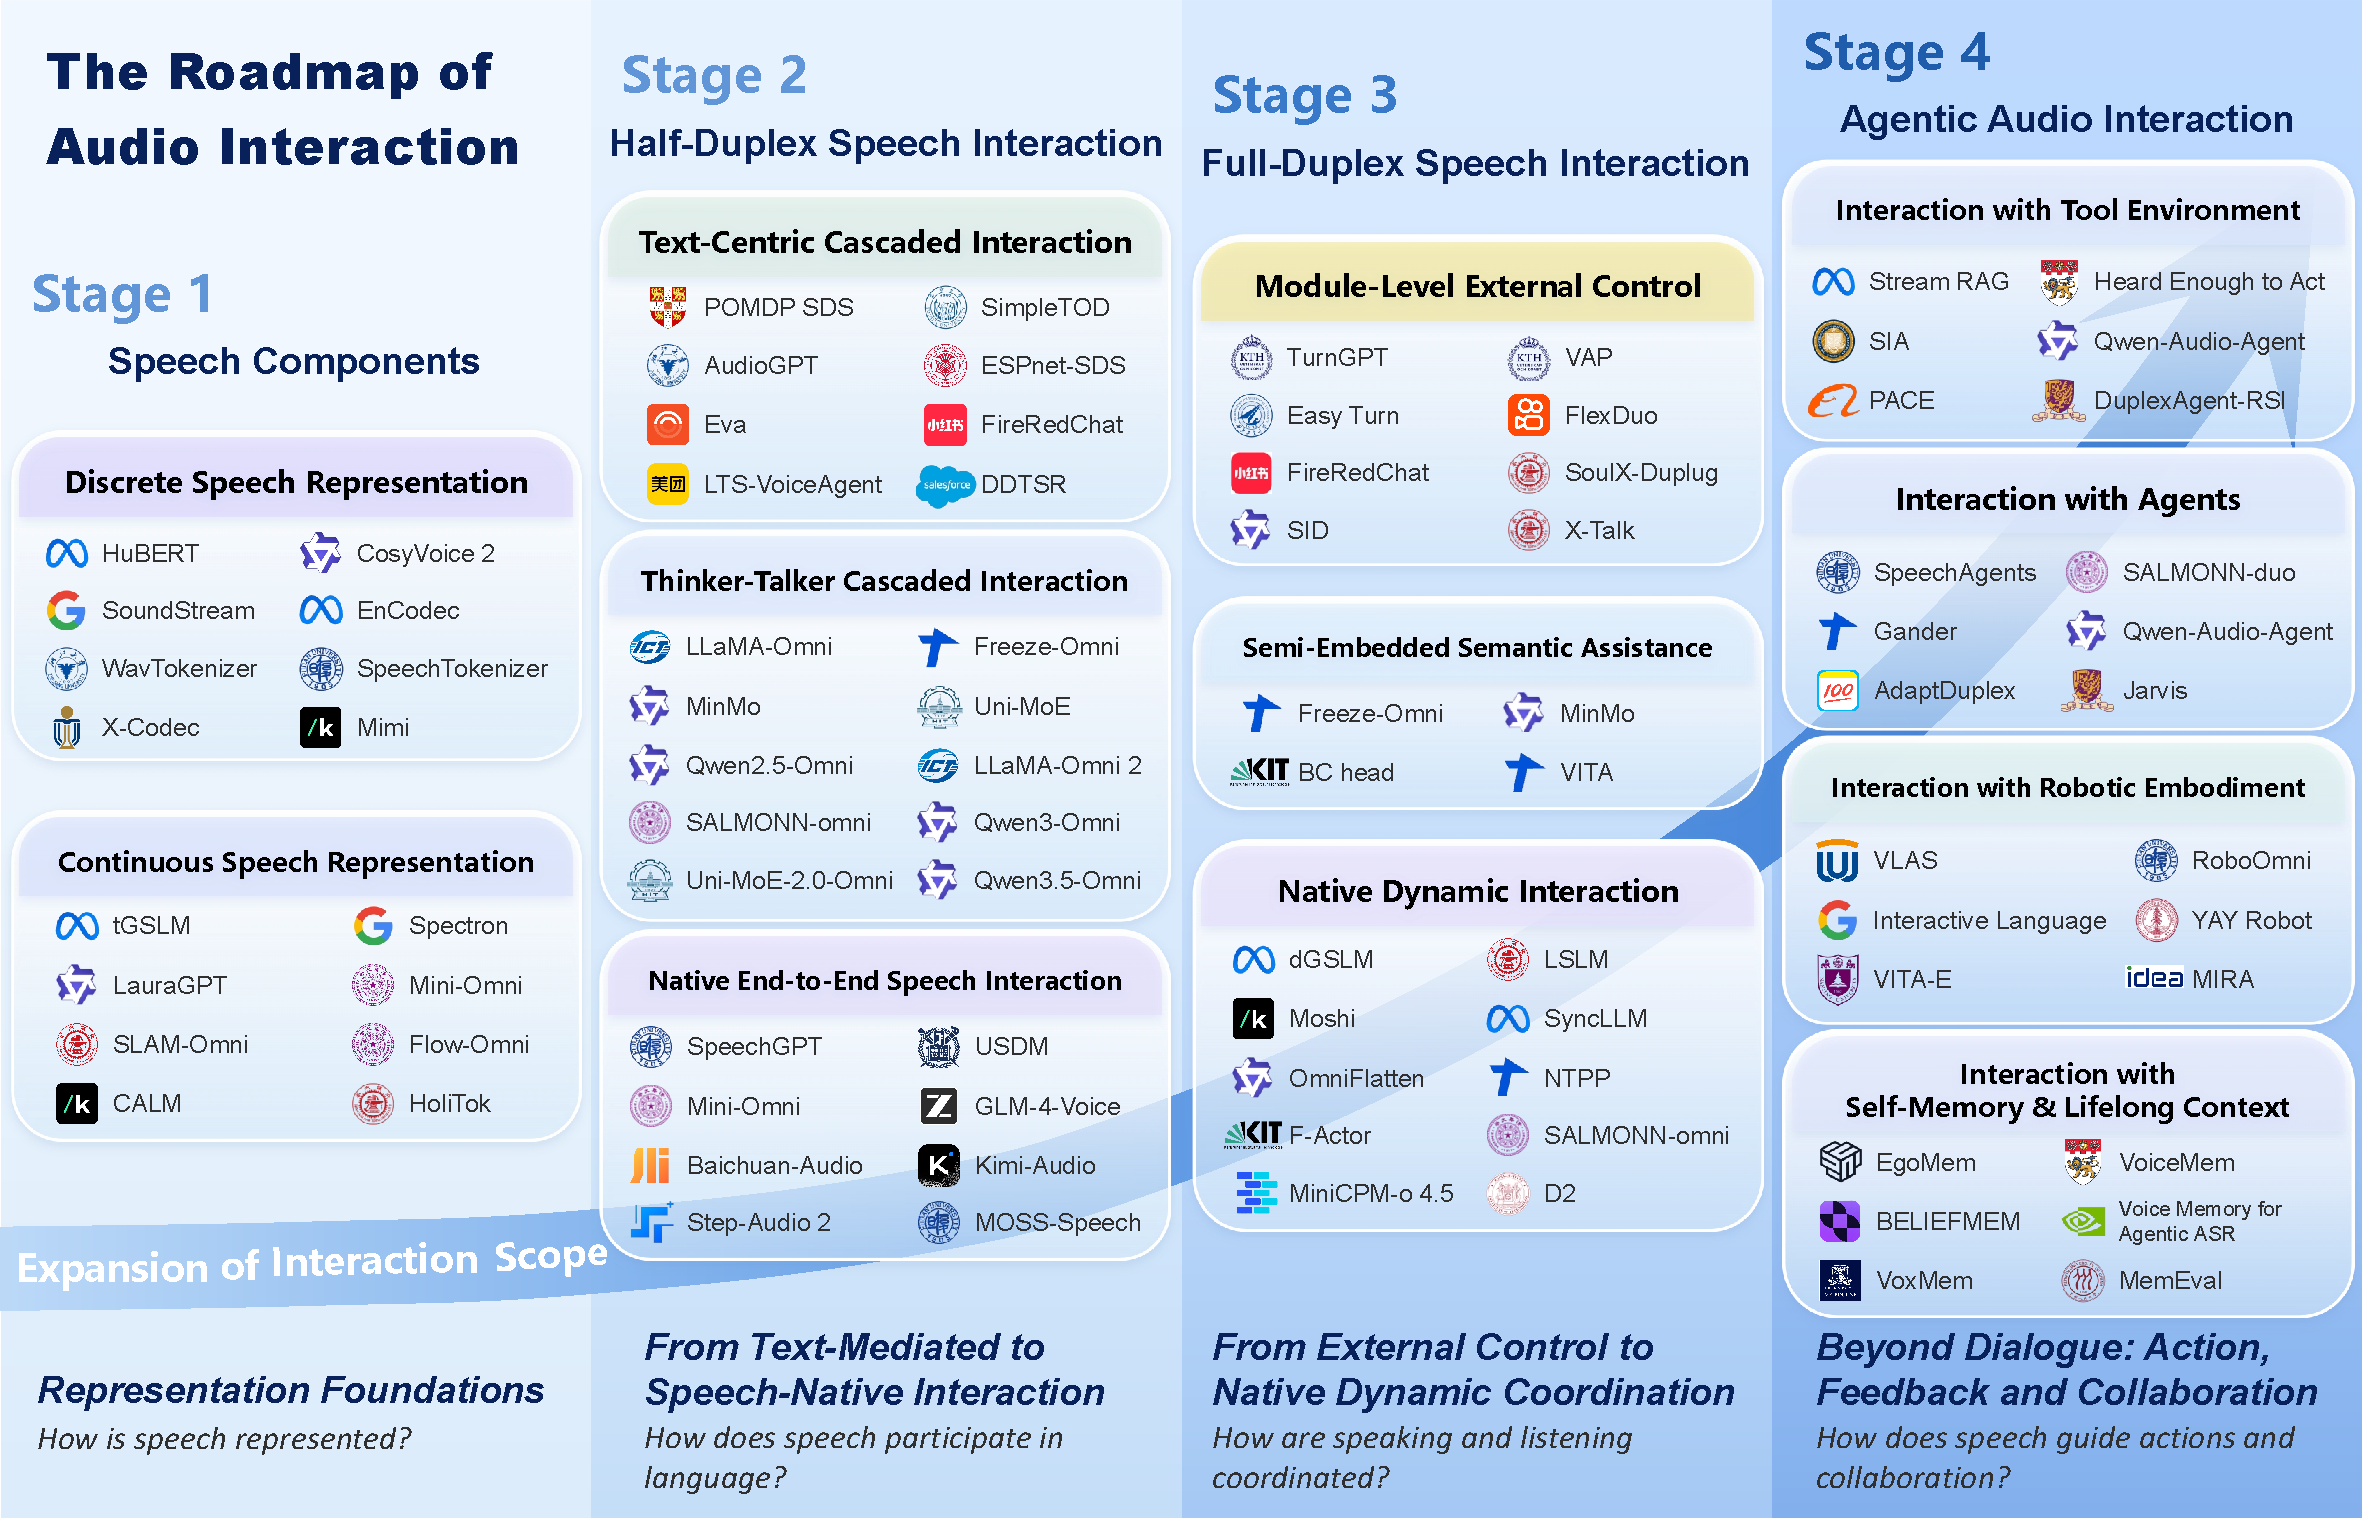
\includegraphics[width=\textwidth,height=0.78\textheight,keepaspectratio]{figures/roadmap_of_audio_interaction.pdf}
    \caption{The roadmap of audio interaction. The vertical arrow traces the expansion in scope from speech representation to language modeling, floor management, and agentic interaction. The horizontal arrow shows increasing internalization in language modeling and floor management.}
    \label{fig:audio-interaction-roadmap}
\end{figure}

Building on this analysis, we consider agentic audio interaction as a forward-looking extension of spoken dialogue. In this outlook, speech provides the primary interface between users and agents, while agents act in digital and physical environments. Existing work on tool use, agent collaboration, robotic embodiment, and persistent memory offers initial foundations for this direction~\cite{DBLP:conf/aaai/HuangLYSCYWHHLR24,DBLP:journals/corr/abs-2401-03945,DBLP:conf/iclr/ZhaoD0GB0W25,DBLP:conf/chi/ZulfikarCM24,DBLP:conf/coling/KirmayrSSMA25}. Through spoken interaction, users can express and refine their goals, while agents communicate the outcomes of their actions and respond to further guidance. The scope of interaction thus expands beyond conversational exchange to encompass actions and environmental feedback, with speech connecting these activities to the user. We examine the capabilities required for speech language models to support this expanded role, distinguishing demonstrated mechanisms from the prospect of sustained collaboration.

% Building on this analysis, we consider agentic audio interaction as a forward-looking extension of spoken dialogue. In this outlook, speech provides the primary interface between users and agents, while agents act in digital and physical environments. Existing work on tool use, agent collaboration, robotic embodiment, and persistent memory offers initial foundations for this direction~\cite{DBLP:conf/aaai/HuangLYSCYWHHLR24,DBLP:journals/corr/abs-2401-03945,DBLP:conf/iclr/ZhaoD0GB0W25,DBLP:conf/chi/ZulfikarCM24,DBLP:conf/coling/KirmayrSSMA25}. Through spoken interaction, users can express and refine their goals, while the system communicates action outcomes and responds to further guidance. We examine how speech interaction models mediate between users' evolving needs and agents' execution capabilities, maintaining continuity between dialogue, action, and feedback.

To complement our analysis of technical approaches, we review training datasets and evaluation benchmarks for speech interaction. We organize these resources around conversational content and timing, reflecting our view that the interaction experience depends on their coordination. The two dimensions cut across technical routes reviewed above, allowing us to examine how training resources support interaction capabilities and which aspects of interaction are captured by existing evaluations.


% \begin{samepage}
% Our contributions are summarized as follows:
% \begin{itemize}
%     \item We present an interaction-centered taxonomy and roadmap of speech language models, covering speech components, half-duplex interaction, and full-duplex interaction. A shared principle of internalization provides a common basis for classifying methods in the SLMs areas.
%     \item We analyze how model designs and training approaches support or constrain interaction, and reviewing datasets and benchmarks along the dimensions of conversational content and timing to clarify what training data support and what current evaluations measure.
%     \item We develop an outlook on agentic audio interaction, examining speech as the primary interface between users and agents and identifying the capabilities needed to extend spoken dialogue toward action and collaboration in digital and physical environments.
% \end{itemize}
% \end{samepage}

\begin{samepage}
Our contributions are summarized as follows:
\begin{itemize}
    \item We present an interaction-centered taxonomy and roadmap of speech language models, covering speech components, half-duplex interaction, and full-duplex interaction. A shared principle of internalization provides a common basis for classifying methods in the SLMs areas.
    \item We analyze how model designs and training approaches support or constrain spoken interaction, highlighting the trade-offs across technical approaches. Base on this, we develop an outlook on agentic audio interaction, examining speech as the primary interface between users and agents and identifying the capabilities needed to extend spoken dialogue toward action and collaboration in digital and physical environments.
    \item We review training datasets and evaluation benchmarks along the dimensions of conversational content and timing. We examine which interaction capabilities the datasets support and what current benchmarks measure.
\end{itemize}
\end{samepage}
\section{Evolving Paradigms of Audio Interaction and Discussion}
\label{sec:interaction_paradigms}


\begin{figure}[!t]
    \centering
    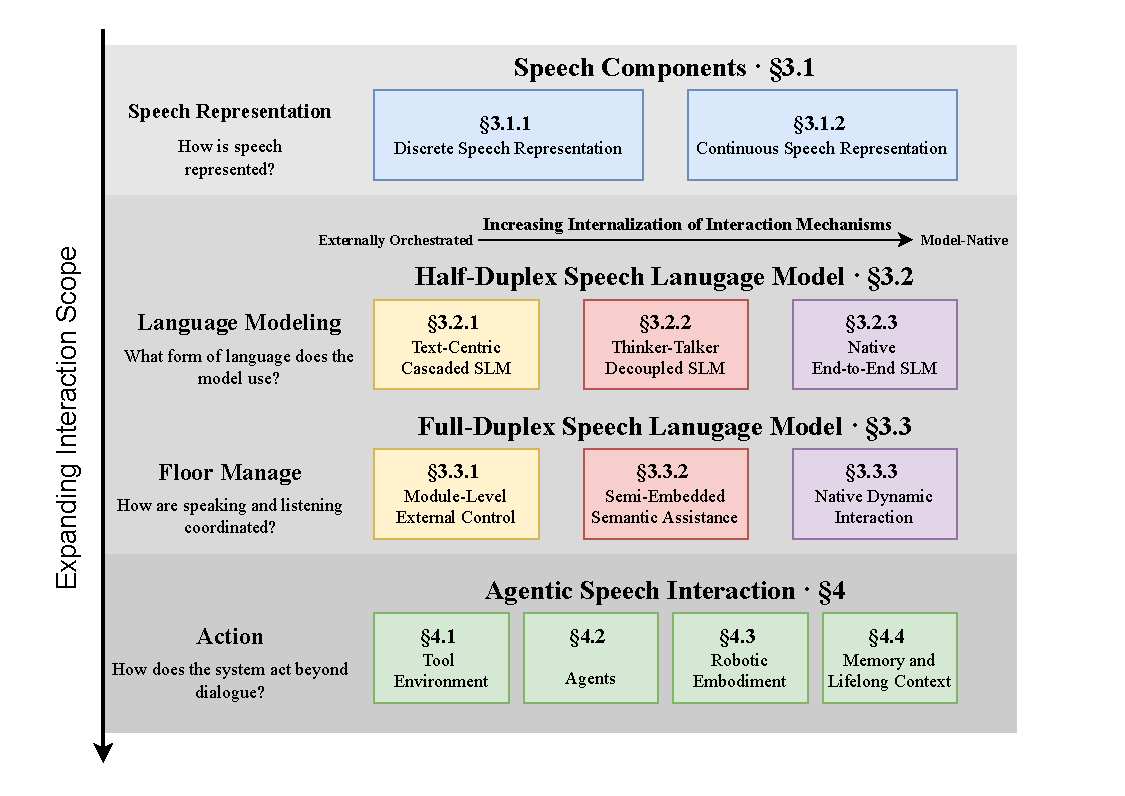
\includegraphics[width=\textwidth,height=0.78\textheight,keepaspectratio]{figures/Taxonomy.pdf}
    \caption{The taxonomy of audio interaction.}
    \label{fig:audio-interaction-taxonomy}
\end{figure}

% Understanding the development of speech interaction requires distinguishing the interaction functions a system supports from the mechanisms that realize them. Figure~\ref{fig:interaction_taxonomy} organizes this distinction along two directions. Vertically, the roadmap expands from speech representation to language interaction, conversational timing, and action beyond dialogue. Horizontally, the taxonomy examines how language interaction and timing control are incorporated into the core interaction model. We refer to this incorporation as the \emph{internalization of interaction mechanisms}. It concerns the role of the core model in a particular interaction function, rather than the number of components or whether the entire system is jointly trained. The roadmap describes an expansion of analytical scope, not a sequence that every system must follow.

Figure~\ref{fig:audio-interaction-taxonomy} distinguishes the scope of interaction from how individual mechanisms are implemented. Vertically, the roadmap begins with speech representation as the technical foundation and extends to action beyond dialogue. Horizontally, we compare designs in language modeling and floor management by the extent to which the core interaction model handles the relevant mechanism. We refer to this organizing principle as the \emph{internalization of interaction mechanisms}. The spectrum runs from externally orchestrated mechanisms to model-native capabilities, with intermediate designs dividing the work between external components and the core model. A system's position on this spectrum is assessed for each mechanism, regardless of its component count or whether the entire system is jointly trained.

\paragraph{Speech Representation: the foundation of speech interaction.}
The first question is how speech enters and leaves the model's representation space. Discrete tokens and continuous representations offer different ways to make acoustic signals available for computation and generation~\cite{DBLP:conf/acl/CuiYJMZWGK25}. Both can retain linguistic and acoustic information, with their usefulness depending on what is preserved, compressed, and made accessible to subsequent modeling. Section~\ref{sec:speech-components} therefore treats discrete and continuous representations as alternative foundations rather than successive levels of interaction intelligence. Representation determines what information is available; the following parts examine how that information participates in interaction.


\paragraph{Language Modeling: the form of language within the interaction model.}
With speech represented, the next concern is whether the core model conducts language interaction through text, speech, or a combination of both. Section~3.2 examines this question within half-duplex dialogue, where users and systems alternate speaking turns. In text-centric cascades, recognition and synthesis surround a text-based dialogue model. Thinker-Talker systems bring speech information directly into understanding, while replies remain organized around text and are realized by a separate speech generator. Native end-to-end speech models extend the role of speech representations into the modeling of both conversational input and output~\cite{}. These distinctions concern the model's medium of language interaction, not simply its output modality. Internalization here describes the extent to which speech participates in the core model's understanding and response formation. Auxiliary text may remain useful in native speech models, and streaming computation can operate within a turn-based interaction policy.

\paragraph{Timing: the coordination of speaking and listening.}
The form of language used by a model does not, by itself, determine how it coordinates with another speaker. Full-duplex interaction brings ongoing input and output into the same conversational process, requiring decisions about when to speak, continue listening, or adjust an unfolding response~\cite{DBLP:conf/emnlp/VeluriPYGG24}. Accordingly, Section~3.3 distinguishes module-level external control, semi-embedded semantic assistance, and native dynamic interaction based on where these decisions are made. Specifically, external controllers manage timing separately from the response model; semi-embedded mechanisms use the model's internal representations to inform control; and native mechanisms incorporate timing decisions into the model's ongoing generation. Here, internalization concerns conversational coordination rather than the use of speech as a language medium; native timing control need not eliminate external audio-processing or serving components. This distinction explains why a native speech model can remain turn-based, while an externally controlled system can support full-duplex behavior. The key distinction, therefore, lies in how conversational timing is determined, not simply how quickly speech is generated.

\paragraph{Action: extending interaction beyond dialogue.}
Agentic audio interaction expands the scope from exchanging utterances to acting on tasks and incorporating their consequences into subsequent interaction. In the outlook developed in Section~4, speech remains the primary interface between users and agents, while agents use tools, collaborate with other agents, act through robotic embodiments, and access persistent memory~\cite{}. These categories identify targets of action rather than levels of internalization, and a system may combine several of them. The extension concerns the relationship between spoken goals, agent actions, and environmental feedback. Speech connects users to this process throughout a task, allowing them to refine intentions and interpret outcomes. We distinguish existing mechanisms from the broader prospect of sustained collaboration; neither tool access nor full-duplex dialogue alone establishes this capability.

Taken together, the roadmap separates the expansion of interaction scope from the internalization of particular mechanisms. Language and timing need not be internalized to the same degree, and action capabilities can be built on either turn-based or full-duplex dialogue. Bringing a mechanism into the core model creates opportunities to learn its dependencies on conversational context, but its effectiveness still depends on representation, training, and execution~\cite{}. External components can retain advantages in controllability and independent optimization. The taxonomy thus supports comparison through what each design makes possible and what it leaves unresolved, rather than treating architectural integration as a universal measure of progress.


\begin{figure*}[tp]
  \centering
  \begin{adjustbox}{
    max totalsize={\textwidth}{0.90\textheight},
    center
  }
  \begin{tikzpicture}[
    taxonomy node/.style={
      draw=gray!65,
      rounded corners=2pt,
      inner sep=4pt,
      font=\scriptsize
    },
    taxonomy detail/.style={
      taxonomy node,
      text width=10.6cm,
      align=left
    },
    taxonomy topic/.style={
      taxonomy node,
      text width=2.4cm,
      align=center
    },
    taxonomy group/.style={
      taxonomy node,
      text width=2.1cm,
      align=center,
      font=\bfseries\scriptsize,
      execute at begin node={\hyphenpenalty=10000\relax}
    },
    taxonomy edge/.style={
      draw=gray!65,
      line width=0.4pt
    }
  ]

  % =========================================================
  % Speech Components
  % =========================================================

  \node[
    taxonomy detail,
    fill=brightlavender!12,
    anchor=north west
  ] (detail0) at (7.25,0) {
    \taxwork{HuBERT}{DBLP:journals/taslp/HsuBTLSM21};
    \taxwork{CosyVoice~2}{DBLP:journals/corr/abs-2412-10117};
    \taxwork{SoundStream}{DBLP:journals/taslp/ZeghidourLOST22};
    \taxwork{EnCodec}{DBLP:journals/tmlr/DefossezCSA23};
    \taxwork{WavTokenizer}{DBLP:conf/iclr/Ji00C0Z0C0LZY0J25};
    \taxwork{SpeechTokenizer}{DBLP:conf/iclr/ZhangZLZQ24};
    \taxwork{X-Codec}{DBLP:conf/aaai/YeSL00DKCPLGX25};
    \taxwork{Mimi}{DBLP:journals/corr/abs-2410-00037};
    \taxwork{DualCodec}{DBLP:conf/interspeech/LiLLHWWZ025}.
  };

  \node[
    taxonomy topic,
    fill=brightlavender!20,
    anchor=west
  ] (topic0) at (4.2,0 |- detail0.west) {
    Discrete Speech Representation
  };
  \draw[taxonomy edge] (topic0.east) -- (detail0.west);

  \node[
    taxonomy detail,
    fill=brightlavender!12,
    anchor=north west
  ] (detail1) at ($(detail0.south west)+(0,-0.2)$) {
    \taxwork{tGSLM}{DBLP:conf/emnlp/AlgayresANCSSD23};
    \taxwork{Spectron}{DBLP:conf/iclr/NachmaniLHSAMRS24};
    \taxwork{LauraGPT}{DBLP:journals/corr/abs-2310-04673};
    \taxwork{Mini-Omni}{DBLP:journals/corr/abs-2408-16725};
    \taxwork{SLAM-Omni}{DBLP:conf/acl/Chen0YLLXN00L0025};
    \taxwork{Flow-Omni}{DBLP:journals/corr/abs-2412-04917};
    \taxwork{Cont-SPT}{DBLP:conf/naacl/LiXSCK25};
    \taxwork{CALM}{DBLP:conf/iclr/RouardORZD26};
    \taxwork{HoliTok}{DBLP:journals/corr/abs-2605-29948}.
  };

  \node[
    taxonomy topic,
    fill=brightlavender!20,
    anchor=west
  ] (topic1) at (4.2,0 |- detail1.west) {
    Continuous Speech Representation
  };
  \draw[taxonomy edge] (topic1.east) -- (detail1.west);

  % =========================================================
  % Half-Duplex Interaction
  % =========================================================

  \node[
    taxonomy detail,
    fill=lightgreen!12,
    anchor=north west
  ] (detail2) at ($(detail1.south west)+(0,-0.4)$) {
    \taxwork{POMDP SDS}{DBLP:journals/pieee/YoungGTW13};
    \taxwork{SimpleTOD}{DBLP:conf/nips/Hosseini-AslMWY20};
    \taxwork{AudioGPT}{DBLP:conf/aaai/HuangLYSCYWHHLR24};
    \taxwork{ESPnet-SDS}{DBLP:conf/naacl/Arora0STCBFKTSS25};
    \taxwork{Eva}{DBLP:conf/ifaamas/QinZ25};
    \taxwork{LiveKit Agents}{livekitagentsdocs};
    \taxwork{Pipecat}{pipecatdocs};
    \taxwork{Schlangen \& Skantze}{DBLP:journals/dad/SchlangenS11};
    \taxwork{InproTK}{DBLP:conf/naacl/BaumannS12};
    \taxwork{Telecom Agent}{DBLP:journals/corr/abs-2508-04721};
    \taxwork{FireRedChat}{DBLP:journals/corr/abs-2509-06502};
    \taxwork{LTS-VoiceAgent}{DBLP:journals/corr/abs-2601-19952};
    \taxwork{DDTSR}{DBLP:journals/corr/abs-2602-23266}.
  };

  \node[
    taxonomy topic,
    fill=lightgreen!20,
    anchor=west
  ] (topic2) at (4.2,0 |- detail2.west) {
    Text-Centric Cascade
  };
  \draw[taxonomy edge] (topic2.east) -- (detail2.west);

  \node[
    taxonomy detail,
    fill=lightgreen!12,
    anchor=north west
  ] (detail3) at ($(detail2.south west)+(0,-0.2)$) {
    \taxwork{LLaMA-Omni}{DBLP:conf/iclr/FangGZMZ025};
    \taxwork{Freeze-Omni}{DBLP:conf/icml/WangLFZS000M25};
    \taxwork{MinMo}{DBLP:journals/corr/abs-2501-06282};
    \taxwork{Uni-MoE}{DBLP:journals/pami/LiJHWZLMZ25};
    \taxwork{Qwen2.5-Omni}{DBLP:journals/corr/abs-2503-20215};
    \taxwork{LLaMA-Omni~2}{DBLP:journals/corr/abs-2505-02625};
    \taxwork{SALMONN-omni}{DBLP:journals/corr/abs-2505-17060};
    \taxwork{Qwen3-Omni}{DBLP:journals/corr/abs-2509-17765};
    \taxwork{Uni-MoE-2.0-Omni}{DBLP:journals/corr/abs-2511-12609};
    \taxwork{Qwen3.5-Omni}{DBLP:journals/corr/abs-2604-15804}.
  };

  \node[
    taxonomy topic,
    fill=lightgreen!20,
    anchor=west
  ] (topic3) at (4.2,0 |- detail3.west) {
    Thinker--Talker Decoupling
  };
  \draw[taxonomy edge] (topic3.east) -- (detail3.west);

  \node[
    taxonomy detail,
    fill=lightgreen!12,
    anchor=north west
  ] (detail4) at ($(detail3.south west)+(0,-0.2)$) {
    \taxwork{SpeechGPT}{DBLP:conf/emnlp/ZhangLZZWZQ23};
    \taxwork{USDM}{DBLP:conf/nips/KimSJKKKLSOHYY24};
    \taxwork{Mini-Omni}{DBLP:journals/corr/abs-2408-16725};
    \taxwork{IntrinsicVoice}{DBLP:journals/corr/abs-2410-08035};
    \taxwork{GLM-4-Voice}{DBLP:journals/corr/abs-2412-02612};
    \taxwork{Flow-Omni}{DBLP:journals/corr/abs-2412-04917};
    \taxwork{SLAM-Omni}{DBLP:conf/acl/Chen0YLLXN00L0025};
    \taxwork{Baichuan-Audio}{DBLP:journals/corr/abs-2502-17239};
    \taxwork{Kimi-Audio}{DBLP:journals/corr/abs-2504-18425};
    \taxwork{VITA-Audio}{DBLP:journals/corr/abs-2505-03739};
    \taxwork{Step-Audio~2}{DBLP:journals/corr/abs-2507-16632};
    \taxwork{MOSS-Speech}{DBLP:conf/iclr/ZhaoXJWCJCLCWZC26}.
  };

  \node[
    taxonomy topic,
    fill=lightgreen!20,
    anchor=west
  ] (topic4) at (4.2,0 |- detail4.west) {
    Native End-to-End Interaction
  };
  \draw[taxonomy edge] (topic4.east) -- (detail4.west);

  % =========================================================
  % Full-Duplex Interaction
  % =========================================================

  \node[
    taxonomy detail,
    fill=lightyellow!12,
    anchor=north west
  ] (detail5) at ($(detail4.south west)+(0,-0.4)$) {
    \taxwork{TurnGPT}{DBLP:conf/emnlp/EkstedtS20};
    \taxwork{RC-TurnGPT}{DBLP:conf/acl/JiangES23};
    \taxwork{VAP}{DBLP:conf/interspeech/EkstedtS22};
    \taxwork{Next-Turn}{DBLP:journals/corr/abs-2606-18094};
    \taxwork{Easy Turn}{DBLP:journals/corr/abs-2509-23938};
    \taxwork{FastTurn}{DBLP:journals/corr/abs-2604-01897};
    \taxwork{FlexDuo}{DBLP:journals/corr/abs-2502-13472};
    \taxwork{FireRedChat}{DBLP:journals/corr/abs-2509-06502};
    \taxwork{SoulX-Duplug}{arXiv:2603.14877};
    \taxwork{SID}{DBLP:journals/corr/abs-2603-24144};
    \taxwork{X-Talk}{DBLP:journals/corr/abs-2512-18706}.
  };

  \node[
    taxonomy topic,
    fill=lightyellow!20,
    anchor=west
  ] (topic5) at (4.2,0 |- detail5.west) {
    Module-Level External Control
  };
  \draw[taxonomy edge] (topic5.east) -- (detail5.west);

  \node[
    taxonomy detail,
    fill=lightyellow!12,
    anchor=north west
  ] (detail6) at ($(detail5.south west)+(0,-0.2)$) {
    \taxwork{Freeze-Omni}{DBLP:conf/icml/WangLFZS000M25};
    \taxwork{MinMo}{DBLP:journals/corr/abs-2501-06282};
    \taxwork{BC head}{DBLP:journals/corr/abs-2609-29418};
    \taxwork{VITA}{DBLP:journals/corr/abs-2408-05211}.
  };

  \node[
    taxonomy topic,
    fill=lightyellow!20,
    anchor=west
  ] (topic6) at (4.2,0 |- detail6.west) {
    Semi-Embedded Semantic Assistance
  };
  \draw[taxonomy edge] (topic6.east) -- (detail6.west);

  \node[
    taxonomy detail,
    fill=lightyellow!12,
    anchor=north west
  ] (detail7) at ($(detail6.south west)+(0,-0.2)$) {
    \taxwork{dGSLM}{DBLP:journals/tacl/NguyenKCAHETASM23};
    \taxwork{LSLM}{DBLP:conf/aaai/MaSDC0WW025};
    \taxwork{Moshi}{DBLP:journals/corr/abs-2410-00037};
    \taxwork{SyncLLM}{DBLP:conf/emnlp/VeluriPYGG24};
    \taxwork{OmniFlatten}{DBLP:conf/acl/ZhangCDCWZLYTDZ25};
    \taxwork{NTPP}{DBLP:journals/corr/abs-2506-00975};
    \taxwork{F-Actor}{DBLP:journals/corr/abs-2601-11329};
    \taxwork{DuplexCascade}{DBLP:journals/corr/abs-2603-09180};
    \taxwork{Raon-SpeechChat}{DBLP:journals/corr/abs-2605-23912};
    \taxwork{SALMONN-omni}{DBLP:journals/corr/abs-2505-17060};
    \taxwork{MiniCPM-o~4.5}{DBLP:journals/corr/abs-2604-27393};
    \taxwork{DuplexOmni}{DBLP:journals/corr/abs-2606-09186};
    \taxwork{BayLing-Duplex}{DBLP:journals/corr/abs-2606-14528};
    \taxwork{Lychee-FD}{DBLP:conf/acl/LiuZLTJCZMXHHLZ26};
    \taxwork{Realtime-Venus}{DBLP:journals/corr/abs-2609-13814};
    \taxwork{AdaptDuplex}{DBLP:journals/corr/abs-2609-29217};
    \taxwork{MultiTalk}{DBLP:journals/corr/abs-2609-36903};
    \taxwork{D2}{arXiv:2610.17124}.
  };

  \node[
    taxonomy topic,
    fill=lightyellow!20,
    anchor=west
  ] (topic7) at (4.2,0 |- detail7.west) {
    Native Dynamic Interaction
  };
  \draw[taxonomy edge] (topic7.east) -- (detail7.west);

  % =========================================================
  % Agentic Interaction
  % =========================================================

  \node[
    taxonomy detail,
    fill=paleblue!12,
    anchor=north west
  ] (detail8) at ($(detail7.south west)+(0,-0.4)$) {
    \taxwork{Spoken Function Calling}{DBLP:journals/corr/abs-2608-05126};
    \taxwork{Stream RAG}{DBLP:journals/corr/abs-2510-02044};
    \taxwork{Heard Enough to Act}{WEB:arxiv/2610.34653};
    \taxwork{SIA}{DBLP:journals/corr/abs-2605-13360};
    \taxwork{Gander}{DBLP:journals/corr/abs-2609-08977};
    \taxwork{StepAudio~3 Realtime}{WEB:arxiv/2609.14005};
    \taxwork{Qwen-Audio-Agent}{DBLP:journals/corr/abs-2609-25195};
    \taxwork{DuplexAgent-RSI}{WEB:arxiv/2610.11299};
    \taxwork{MoshiRAG}{tool_chien2026moshirag};
    \taxwork{PACE}{DBLP:journals/corr/abs-2608-07631};
    \taxwork{$\tau$-Voice}{tool_ray2026tauvoice};
    \taxwork{Qwen3.5-Omni}{DBLP:journals/corr/abs-2604-15804};
    \taxwork{VoiceChat}{DBLP:journals/corr/abs-2609-21967};
    \taxwork{DuplexSLA}{DBLP:journals/corr/abs-2605-20755};
    \taxwork{Frontend--Backend}{DBLP:journals/corr/abs-2609-19334};
    \taxwork{SALMONN-duo}{DBLP:journals/corr/abs-2609-34247};
    \taxwork{VoxMind}{DBLP:conf/acl/LiangCJCJLZPLZ26};
    \taxwork{SpeechGym}{DBLP:journals/corr/abs-2608-26432}.
  };

  \node[
    taxonomy topic,
    fill=paleblue!20,
    anchor=west
  ] (topic8) at (4.2,0 |- detail8.west) {
    Tool Environment
  };
  \draw[taxonomy edge] (topic8.east) -- (detail8.west);

  \node[
    taxonomy detail,
    fill=paleblue!12,
    anchor=north west
  ] (detail9) at ($(detail8.south west)+(0,-0.2)$) {
    \taxwork{SpeechAgents}{DBLP:journals/corr/abs-2401-03945};
    \taxwork{Interaction Models}{WEB:thinkingmachines/interaction-models};
    \taxwork{SALMONN-duo}{DBLP:journals/corr/abs-2609-34247};
    \taxwork{Gander}{DBLP:journals/corr/abs-2609-08977};
    \taxwork{VoxMind}{DBLP:conf/acl/LiangCJCJLZPLZ26};
    \taxwork{Qwen-Audio-Agent}{DBLP:journals/corr/abs-2609-25195};
    \taxwork{AdaptDuplex}{DBLP:journals/corr/abs-2609-29217};
    \taxwork{Jarvis}{WEB:arxiv/2610.23804}.
  };

  \node[
    taxonomy topic,
    fill=paleblue!20,
    anchor=west
  ] (topic9) at (4.2,0 |- detail9.west) {
    Agents
  };
  \draw[taxonomy edge] (topic9.east) -- (detail9.west);

  \node[
    taxonomy detail,
    fill=paleblue!12,
    anchor=north west
  ] (detail10) at ($(detail9.south west)+(0,-0.2)$) {
    \taxwork{Multimodal SR for Embodied Agents}{emb_chang2023};
    \taxwork{Multimodal Human--Autonomous Interaction}{emb_nwankwo2024};
    \taxwork{NMM-HRI}{emb_lai2025nmm};
    \taxwork{VLAS}{emb_zhao2025vlas};
    \taxwork{RoboOmni}{emb_wang2025roboomni};
    \taxwork{KnowNo}{emb_ren2023knowno};
    \taxwork{Interactive Language}{emb_lynch2022interactive};
    \taxwork{YAY Robot}{emb_shi2024yay};
    \taxwork{Incremental Language Understanding}{emb_abrams2025incremental};
    \taxwork{HEAR}{emb_nie2026hear};
    \taxwork{ELLSA}{emb_wang2026ellsa};
    \taxwork{VITA-E}{emb_liu2025vitae};
    \taxwork{MIRA}{emb_lin2026mira};
    \taxwork{Pepper LLM Framework}{emb_studerus2026pepper}.
  };

  \node[
    taxonomy topic,
    fill=paleblue!20,
    anchor=west
  ] (topic10) at (4.2,0 |- detail10.west) {
    Robotic Embodiment
  };
  \draw[taxonomy edge] (topic10.east) -- (detail10.west);

  \node[
    taxonomy detail,
    fill=paleblue!12,
    anchor=north west
  ] (detail11) at ($(detail10.south west)+(0,-0.2)$) {
    \taxwork{EgoMem}{DBLP:journals/corr/abs-2509-11914};
    \taxwork{VoiceMem}{DBLP:journals/corr/abs-2608-26005};
    \taxwork{VoiceTrace}{DBLP:journals/corr/abs-2609-18521};
    \taxwork{SpeakerMem-R1}{DBLP:journals/corr/abs-2609-26780};
    \taxwork{VoxPolyMem}{jia2026voxpolymem};
    \taxwork{Zep}{DBLP:journals/corr/abs-2501-13956};
    \taxwork{BELIEFMEM}{meng-etal-2026-beliefmem};
    \taxwork{APEX-MEM}{DBLP:conf/acl/BanerjeeMSMC26};
    \taxwork{TSHMem}{xu-etal-2026-tshmem};
    \taxwork{Voice Memory for Agentic ASR}{yang2026voicememory};
    \taxwork{Forgetting Without Restarting}{DBLP:journals/corr/abs-2609-04875};
    \taxwork{LongMemEval}{DBLP:conf/iclr/WuWYZCY25};
    \taxwork{VoxMem}{DBLP:journals/corr/abs-2609-32607};
    \taxwork{ContextDialog}{DBLP:journals/corr/abs-2502-19759};
    \taxwork{ChronoScope}{DBLP:conf/acl/AtriJH26};
    \taxwork{MemEval}{wang-etal-2026-memories};
    \taxwork{UTILMEM}{qing-etal-2026-utilmem}.
  };

  \node[
    taxonomy topic,
    fill=paleblue!20,
    anchor=west
  ] (topic11) at (4.2,0 |- detail11.west) {
    Self-Memory and Lifelong Context
  };
  \draw[taxonomy edge] (topic11.east) -- (detail11.west);

  % =========================================================
  % First-level groups
  % =========================================================

  \coordinate (groupcenter0)
    at ($(topic0.west)!0.5!(topic1.west)$);

  \node[
    taxonomy group,
    fill=brightlavender!30,
    anchor=west
  ] (group0) at (1.45,0 |- groupcenter0) {
    Speech Components
  };

  \draw[taxonomy edge]
    (group0.east) -- ++(0.25,0) |- (topic0.west);
  \draw[taxonomy edge]
    (group0.east) -- ++(0.25,0) |- (topic1.west);

  \coordinate (groupcenter1)
    at ($(topic2.west)!0.5!(topic4.west)$);

  \node[
    taxonomy group,
    fill=lightgreen!30,
    anchor=west
  ] (group1) at (1.45,0 |- groupcenter1) {
    Half-Duplex Interaction
  };

  \draw[taxonomy edge]
    (group1.east) -- ++(0.25,0) |- (topic2.west);
  \draw[taxonomy edge]
    (group1.east) -- ++(0.25,0) |- (topic3.west);
  \draw[taxonomy edge]
    (group1.east) -- ++(0.25,0) |- (topic4.west);

  \coordinate (groupcenter2)
    at ($(topic5.west)!0.5!(topic7.west)$);

  \node[
    taxonomy group,
    fill=lightyellow!30,
    anchor=west
  ] (group2) at (1.45,0 |- groupcenter2) {
    Full-Duplex Interaction
  };

  \draw[taxonomy edge]
    (group2.east) -- ++(0.25,0) |- (topic5.west);
  \draw[taxonomy edge]
    (group2.east) -- ++(0.25,0) |- (topic6.west);
  \draw[taxonomy edge]
    (group2.east) -- ++(0.25,0) |- (topic7.west);

  \coordinate (groupcenter3)
    at ($(topic8.west)!0.5!(topic11.west)$);

  \node[
    taxonomy group,
    fill=paleblue!30,
    anchor=west
  ] (group3) at (1.45,0 |- groupcenter3) {
    Agentic Interaction
  };

  \draw[taxonomy edge]
    (group3.east) -- ++(0.25,0) |- (topic8.west);
  \draw[taxonomy edge]
    (group3.east) -- ++(0.25,0) |- (topic9.west);
  \draw[taxonomy edge]
    (group3.east) -- ++(0.25,0) |- (topic10.west);
  \draw[taxonomy edge]
    (group3.east) -- ++(0.25,0) |- (topic11.west);

  % =========================================================
  % Root
  % =========================================================

  \coordinate (rootcenter)
    at ($(group0.west)!0.5!(group3.west)$);

  \node[
    taxonomy node,
    fill=gray!12,
    rotate=90
  ] (root) at (0.45,0 |- rootcenter) {
    \textbf{Audio Interaction}
  };

  \foreach \g in {0,...,3}{
    \draw[taxonomy edge]
      (root.south)
      -- (1.1,0 |- root.south)
      |- (group\g.west);
  }

  \end{tikzpicture}
  \end{adjustbox}

  \caption{
    Taxonomy of audio interaction models and related methods,
    organized into speech components, half-duplex interaction,
    full-duplex interaction, and agentic audio interaction.
    Each subcategory lists representative works with references.
    A work may appear in more than one branch.
  }
  \label{fig:taxonomy-audio-interaction}
\end{figure*}

\section{Roadmap of Audio Interaction}
\label{roadmap}

% The four taxonomy layers are organized as subsections, following the roadmap structure of the reference survey.
\subsection{Speech Components}
\label{sec:speech-components}

Our interaction roadmap begins with speech components, which bridge speech signals and model representations to support perception and generation. Speech can be represented either as discrete units obtained through encoding and quantization or as sequences of continuous vectors, giving rise to discrete and continuous speech representations, respectively. Across both representation types, we examine how component designs preserve speech information, support downstream modeling, and manage computational cost. For discrete representations, we review tokenization designs that emphasize semantic content, acoustic detail, or their combination; for continuous representations, we examine the encoding and decoding interfaces that connect speech with language models. Figure~\ref{fig:speech-components} provides an overview of discrete and continuous speech representations and their associated components. Table~\ref{tab:speech-components} summarizes representative speech components and systems, highlighting their representations and key design choices.

\begin{figure}[htbp]
    \centering
    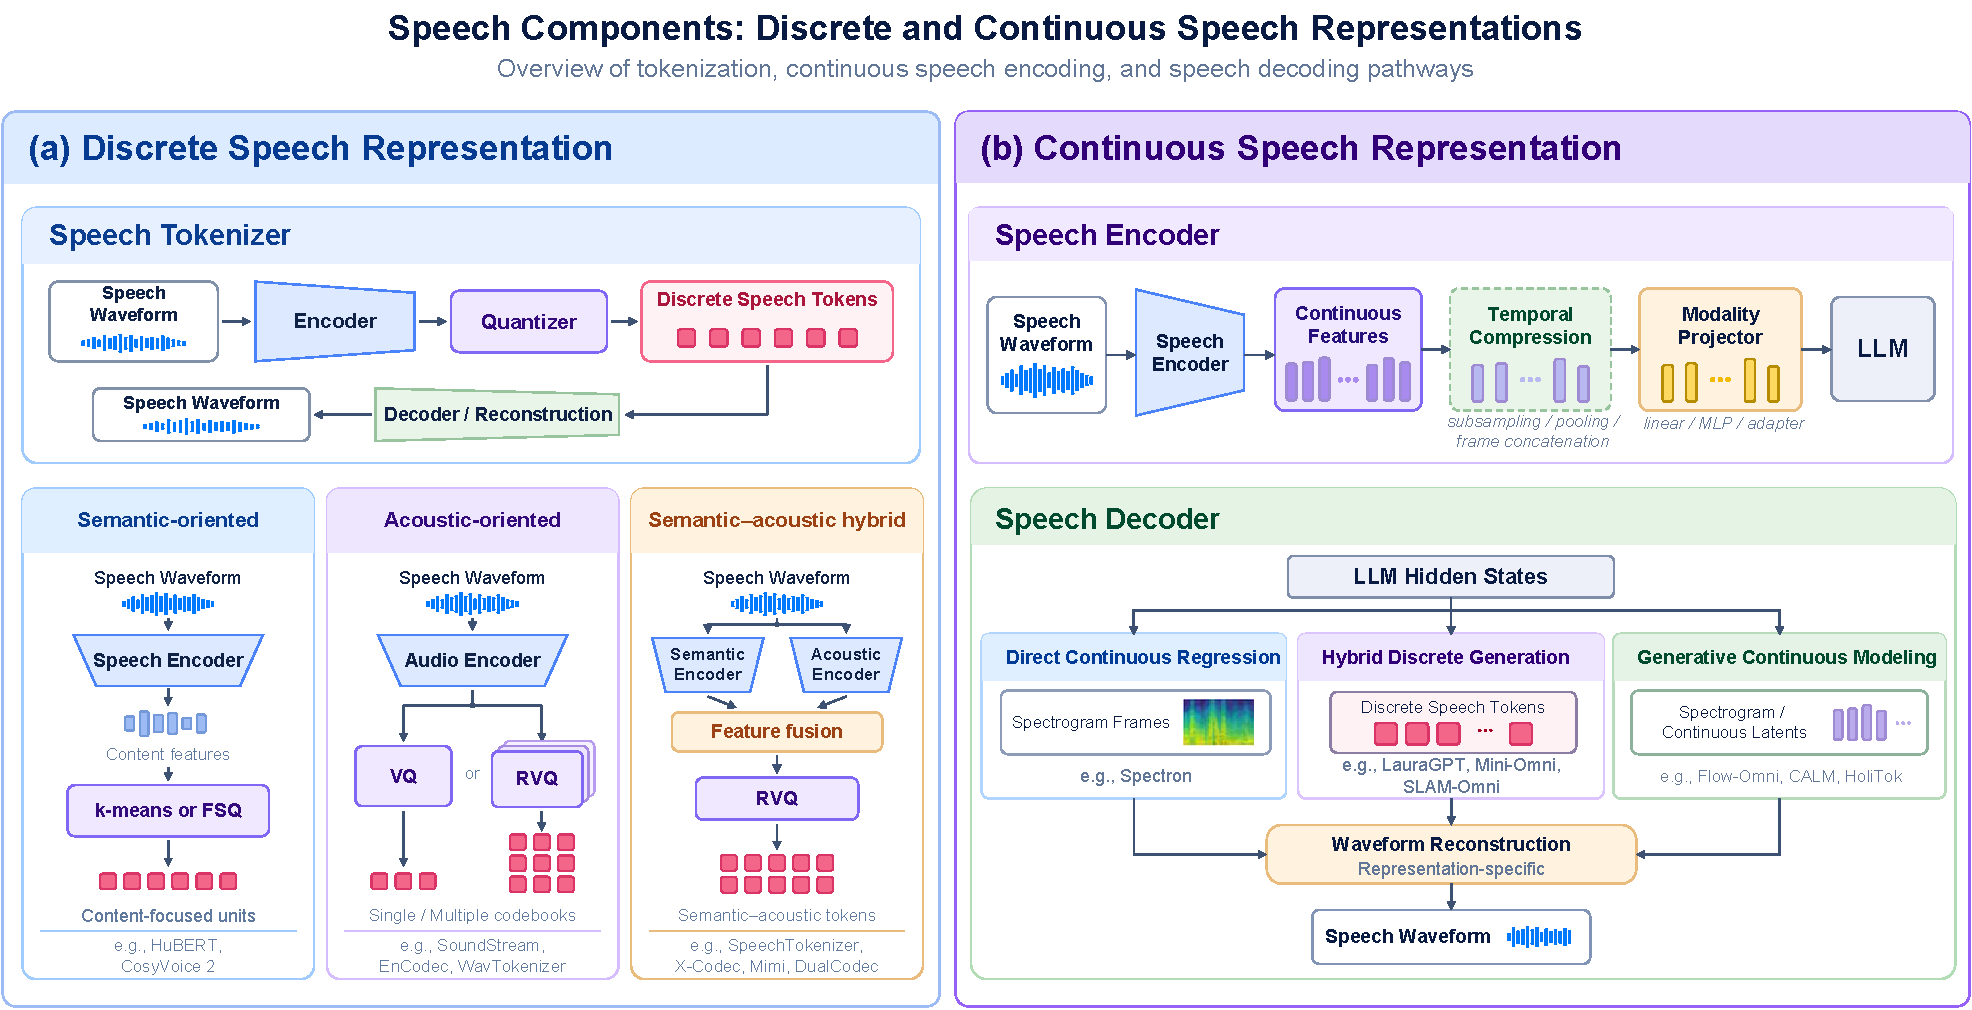
\includegraphics[width=\textwidth]{figures/speech_components.pdf}
    \caption{Overview of speech components for discrete and continuous speech representations. (a) Discrete speech tokenization with semantic-oriented, acoustic-oriented, and semantic--acoustic hybrid designs. (b) Continuous speech representation, comprising speech encoding (top) and speech decoding (bottom). The encoder pathway combines feature extraction, optional temporal compression, and modality projection; the decoder pathways include direct continuous regression, hybrid discrete generation, and generative continuous modeling. The hybrid pathway combines continuous speech input with discrete output tokens.}
    \label{fig:speech-components}
\end{figure}

\subsubsection{Discrete Speech Representation}
\label{sec:discrete-speech-representation}

Discrete speech representations are obtained by encoding and quantizing speech waveforms into sequences of discrete tokens drawn from a finite vocabulary. This enables speech models to adopt the autoregressive modeling and training mechanisms used in large language models (LLMs). The resulting tokens can be converted back into speech through a suitable decoding module~\citep{DBLP:conf/acl/CuiYJMZWGK25}. The core design trade-offs concern sequence length, linguistic content preservation, and acoustic fidelity~\citep{DBLP:journals/pami/GuoLWLSZDCLY26,DBLP:journals/tmlr/MousaviMMPSWYKPMRELLSWK25}. Based on their relative emphasis on linguistic content and acoustic reconstruction, we group existing methods into three broad categories: semantic-oriented, acoustic-oriented, and semantic--acoustic hybrid approaches, as illustrated in Figure~\ref{fig:speech-components}(a)~\citep{DBLP:conf/acl/CuiYJMZWGK25,DBLP:journals/pami/GuoLWLSZDCLY26}.

\textbf{Semantic-oriented.} These methods prioritize linguistic content, typically extracting features from self-supervised or speech recognition models and converting them into discrete units through clustering or quantization. HuBERT learns representations by predicting cluster-based pseudo-labels at masked positions; its hidden features can subsequently be clustered using k-means to obtain content-related speech tokens~\citep{DBLP:journals/taslp/HsuBTLSM21}. CosyVoice 2 incorporates finite scalar quantization (FSQ) into its speech recognition encoder: recognition supervision encourages content preservation, whereas FSQ improves codebook utilization~\citep{DBLP:journals/corr/abs-2412-10117}. These units support downstream content modeling and can reduce sequence length when combined with temporal compression. However, they do not guarantee the preservation of fine acoustic detail; waveform generation commonly relies on additional acoustic modeling or reference conditioning to supply timbre and prosody~\citep{DBLP:journals/pami/GuoLWLSZDCLY26,DBLP:journals/corr/abs-2412-10117}.

\textbf{Acoustic-oriented.} These methods prioritize reconstruction quality and typically adopt an encoder--quantizer--decoder architecture. SoundStream and EnCodec use residual vector quantization (RVQ) to progressively encode residual information in latent features, combining reconstruction and adversarial objectives to preserve acoustic detail~\citep{DBLP:journals/taslp/ZeghidourLOST22,DBLP:journals/tmlr/DefossezCSA23}. WavTokenizer explores a single-codebook alternative, improving the quantization space and decoder to reduce the number of discrete indices while maintaining reconstruction quality~\citep{DBLP:conf/iclr/Ji00C0Z0C0LZY0J25}. This favors high-fidelity synthesis, but reconstruction quality does not ensure that linguistic content is readily modeled. Multi-codebook designs also increase the number of indices per frame and, when serialized, the sequence length, requiring downstream models to balance acoustic fidelity against prediction cost~\citep{DBLP:conf/iclr/ZhangZLZQ24,DBLP:conf/aaai/YeSL00DKCPLGX25,DBLP:journals/corr/abs-2410-00037}.

\textbf{Semantic--acoustic hybrid.} These methods combine semantic supervision with acoustic reconstruction to balance content preservation and acoustic fidelity. SpeechTokenizer distills HuBERT representations into the first RVQ layer, encouraging it to capture linguistic content while subsequent layers encode additional acoustic detail~\citep{DBLP:conf/iclr/ZhangZLZQ24}. X-Codec fuses semantic and acoustic features before quantization and introduces a semantic reconstruction loss~\citep{DBLP:conf/aaai/YeSL00DKCPLGX25}. Mimi organizes semantic vector quantization and acoustic RVQ in parallel, combining low-frame-rate representations with causal encoding and decoding for streaming operation~\citep{DBLP:journals/corr/abs-2410-00037}. DualCodec uses separate speech-representation and waveform encoding streams, enriching the first codec layer with content-related information while the remaining layers encode residual acoustic information~\citep{DBLP:conf/interspeech/LiLLHWWZ025}. These designs provide a shared interface for content modeling and speech generation, but must allocate finite representation capacity between linguistic and acoustic information. A lower frame rate does not necessarily reduce the total prediction workload: codebook count and generation factorization also matter. Likewise, layer-wise specialization should not be interpreted as complete information disentanglement~\citep{DBLP:conf/iclr/ZhangZLZQ24,DBLP:journals/corr/abs-2410-00037,DBLP:conf/interspeech/LiLLHWWZ025}.

Together, these approaches offer different trade-offs among linguistic content, acoustic detail, and modeling cost. For real-time interaction, their suitability depends jointly on token frame rate, codebook count, generation factorization, causality, and look-ahead requirements, rather than compression ratio or offline reconstruction quality alone~\citep{DBLP:journals/taslp/ZeghidourLOST22,DBLP:journals/corr/abs-2410-00037}.


\subsubsection{Continuous Speech Representation}
\label{sec:continuous-speech-representation}

Continuous speech representations model speech as sequences of real-valued vectors rather than indices from a finite codebook. Avoiding explicit quantization can help preserve fine-grained semantic, prosodic, timbral, and other paralinguistic information~\citep{DBLP:journals/corr/abs-2310-04673,DBLP:conf/naacl/LiXSCK25}. Their integration with text-based LLMs nevertheless requires adaptations to representation alignment and, when continuous values are predicted, to the output and sampling mechanisms. Sequence compression, cross-modal alignment, and continuous-space generation therefore constitute central design challenges~\citep{DBLP:conf/emnlp/AlgayresANCSSD23,DBLP:conf/iclr/NachmaniLHSAMRS24,DBLP:journals/corr/abs-2310-04673,DBLP:journals/corr/abs-2412-04917}.

Early work such as tGSLM demonstrated language modeling with continuous speech embeddings, using a learnable Lexical Embedder, contrastive loss, and k-nearest-neighbor (k-NN) sampling~\citep{DBLP:conf/emnlp/AlgayresANCSSD23}. When continuous representations are integrated with pretrained LLMs, these modeling questions extend to two component interfaces: speech encoders provide continuous input representations, while speech decoders convert model outputs into speech.

\paragraph{Speech Encoder}
\label{sec:speech-encoder}

A typical continuous input pathway combines speech feature extraction, temporal compression, and modality projection, as shown in Figure~\ref{fig:speech-components}(b). The speech encoder extracts continuous acoustic and semantic features; subsampling, pooling, or frame concatenation can reduce their sequence length before a linear projection or multilayer perceptron (MLP) adapter maps them into the LLM embedding space. Temporal compression limits the computational cost of high-frame-rate inputs, while modality projection enables the language model to process speech representations~\citep{DBLP:conf/iclr/NachmaniLHSAMRS24,DBLP:journals/corr/abs-2408-16725,DBLP:conf/acl/Chen0YLLXN00L0025}.

Spectron follows a direct implementation of this interface: a pretrained speech encoder produces continuous features, and a projection layer maps them into the language model's embedding space without first converting them into discrete speech tokens~\citep{DBLP:conf/iclr/NachmaniLHSAMRS24}. LauraGPT, Mini-Omni, and SLAM-Omni follow a similar encoder--adapter interface, extracting continuous speech features with a Conformer (LauraGPT) or Whisper encoder (Mini-Omni and SLAM-Omni) and mapping them into the language model's embedding space through adapters or projection layers~\citep{DBLP:journals/corr/abs-2310-04673,DBLP:journals/corr/abs-2408-16725,DBLP:conf/acl/Chen0YLLXN00L0025}. Across these designs, the main interface challenge is to preserve useful speech information while controlling sequence length and aligning the resulting features with the language model.

\paragraph{Speech Decoder}
\label{sec:speech-decoder}

Speech generation maps language model states to acoustic representations and ultimately to waveforms. The speech decoder pathways in Figure~\ref{fig:speech-components}(b) include direct continuous regression, hybrid discrete generation, and generative continuous modeling. In direct continuous regression, Spectron generates text before autoregressively predicting spectrogram frames, which a vocoder converts into a waveform~\citep{DBLP:conf/iclr/NachmaniLHSAMRS24}. Although this approach avoids codec quantization, frame-level generation results in long acoustic sequences and substantial computational overhead. Moreover, the sequential generation of text and spectrogram frames poses challenges for streaming generation. Continuous input representations can also be paired with discrete output tokens, as in the hybrid discrete generation approaches adopted by LauraGPT, Mini-Omni, and SLAM-Omni~\citep{DBLP:journals/corr/abs-2310-04673,DBLP:journals/corr/abs-2408-16725,DBLP:conf/acl/Chen0YLLXN00L0025}. Their speech encoders produce continuous speech representations, while their generation modules autoregressively predict discrete speech tokens, such as codec or semantic tokens.

In generative continuous modeling, Flow-Omni combines a pretrained autoregressive LLM with a lightweight generation module trained using flow matching~\citep{DBLP:journals/corr/abs-2412-04917}. Conditioned on language model states, the module models a distribution over continuous acoustic representations instead of directly regressing a single target frame. CALM uses continuous latents from an audio variational autoencoder (VAE), with a Transformer providing contextual representations that condition a consistency-based generation module~\citep{DBLP:conf/iclr/RouardORZD26}. Related work also explores the continuous representations used for speech generation: Cont-SPT develops a continuous speech tokenizer for text-to-speech (TTS)~\citep{DBLP:conf/naacl/LiXSCK25}, while HoliTok explores a shared continuous latent space for speech understanding and generation~\citep{DBLP:journals/corr/abs-2605-29948}.

Together, the encoder and decoder interfaces connect continuous speech representations to perception and generation. Encoders extract, compress, and align speech features for the language model, while decoders generate speech from model outputs. The design of these interfaces influences how information preserved from the input is reflected in response content and acoustic expression.

\begin{TakeawayBox}{Takeaways: Speech Components}

Discrete speech representations offer complementary trade-offs: semantic-oriented units emphasize content, acoustic-oriented codes emphasize reconstruction, and hybrid designs combine both under representation and prediction constraints. Continuous representations avoid explicit quantization but require suitable alignment and continuous-output modeling. Across both approaches, information preservation must be evaluated together with sequence structure and downstream computation.
\end{TakeawayBox}

\begin{table*}[!htbp]
    \centering
    \caption{Overview of speech component methods and representative systems.
    RVQ: residual vector quantization; FSQ: finite scalar quantization;
    VAE: variational autoencoder.}
    \label{tab:speech-components}
    \footnotesize
    \setlength{\tabcolsep}{3pt}
    \renewcommand{\arraystretch}{1.0}
    \setlength{\defaultaddspace}{2pt}
    \begin{tabular}{@{}
        >{\raggedright\arraybackslash}p{\dimexpr0.18\linewidth-6pt\relax}
        >{\raggedright\arraybackslash}p{\dimexpr0.14\linewidth-6pt\relax}
        >{\raggedright\arraybackslash}p{\dimexpr0.28\linewidth-6pt\relax}
        >{\raggedright\arraybackslash}p{\dimexpr0.40\linewidth-6pt\relax}@{}}
        \toprule
        \textbf{Representation} & \textbf{Component} & \textbf{Work} & \textbf{Highlight} \\
        \midrule
        Discrete & Semantic tokenizer & HuBERT~\citep{DBLP:journals/taslp/HsuBTLSM21} &
        Content-related units support linguistic modeling; reconstruction needs an additional decoder. \\
        \addlinespace
        Discrete & Semantic tokenizer & CosyVoice 2~\citep{DBLP:journals/corr/abs-2412-10117} &
        Recognition supervision preserves content; FSQ improves utilization; synthesis uses acoustic conditioning. \\
        \addlinespace
        Discrete & Acoustic tokenizer & SoundStream~\citep{DBLP:journals/taslp/ZeghidourLOST22}; EnCodec~\citep{DBLP:journals/tmlr/DefossezCSA23} &
        RVQ preserves acoustic detail but increases the number of per-frame prediction targets. \\
        \addlinespace
        Discrete & Acoustic tokenizer & WavTokenizer~\citep{DBLP:conf/iclr/Ji00C0Z0C0LZY0J25} &
        Single-codebook compression reduces prediction targets while prioritizing reconstruction quality. \\
        \addlinespace
        Discrete & Semantic--\newline acoustic\newline hybrid tokenizer & SpeechTokenizer~\citep{DBLP:conf/iclr/ZhangZLZQ24} &
        First-layer distillation emphasizes content; later RVQ layers supply acoustic detail. \\
        \addlinespace
        Discrete & Semantic--\newline acoustic\newline hybrid tokenizer & X-Codec~\citep{DBLP:conf/aaai/YeSL00DKCPLGX25} &
        Joint quantization and semantic reconstruction combine content cues with acoustic fidelity. \\
        \addlinespace
        Discrete & Semantic--\newline acoustic\newline hybrid tokenizer & Mimi~\citep{DBLP:journals/corr/abs-2410-00037} &
        Causal, low-frame-rate coding supports streaming; multiple codebooks retain prediction overhead. \\
        \addlinespace
        Discrete & Semantic--\newline acoustic\newline hybrid tokenizer & DualCodec~\citep{DBLP:conf/interspeech/LiLLHWWZ025} &
        Dual encoding enriches first-layer content; low frame rate shortens temporal sequences. \\
        \midrule
        Continuous & Embedding model & tGSLM~\citep{DBLP:conf/emnlp/AlgayresANCSSD23} &
        Word-sized embeddings, contrastive training, and nearest-neighbor sampling. \\
        \addlinespace
        Continuous & Encoder; decoder & Spectron~\citep{DBLP:conf/iclr/NachmaniLHSAMRS24} &
        Projects speech features into the LLM; predicts spectrogram frames after text. \\
        \addlinespace
        Continuous input;\newline discrete output & Encoder; decoder & LauraGPT~\citep{DBLP:journals/corr/abs-2310-04673} &
        Conformer input features with discrete codec-code generation. \\
        \addlinespace
        Continuous input;\newline discrete output & Encoder; decoder & Mini-Omni~\citep{DBLP:journals/corr/abs-2408-16725} &
        Whisper encoder and audio adapter with discrete audio-token generation. \\
        \addlinespace
        Continuous input;\newline discrete output & Encoder; decoder & SLAM-Omni~\citep{DBLP:conf/acl/Chen0YLLXN00L0025} &
        Downsampled Whisper features and linear projection; semantic-token output. \\
        \addlinespace
        Continuous output & Generation module & Flow-Omni~\citep{DBLP:journals/corr/abs-2412-04917} &
        LLM states condition flow matching over acoustic representations. \\
        \addlinespace
        Continuous & Tokenizer & Cont-SPT~\citep{DBLP:conf/naacl/LiXSCK25} &
        Continuous speech vectors avoid discrete quantization for TTS. \\
        \addlinespace
        Continuous & Latent model; generator & CALM~\citep{DBLP:conf/iclr/RouardORZD26} &
        Audio VAE latents with context-conditioned, consistency-based generation. \\
        \addlinespace
        Continuous & Shared tokenizer & HoliTok~\citep{DBLP:journals/corr/abs-2605-29948} &
        Compact shared latents support both speech understanding and generation. \\
        \bottomrule
    \end{tabular}
\end{table*}


\subsection{Half-Duplex Speech Interaction}
\label{sec:half-duplex}

Building on the preceding speech representations and components,
half-duplex systems organize perception and generation into
turn-based dialogue.
Within speech dialogue, core model modalities define three categories:
text-to-text in cascaded systems, speech-to-text in Thinker-Talker
systems, and speech-to-speech representation modeling in native
end-to-end systems.
This progression shifts text from mediating both input and output
to organizing replies after direct speech perception, then brings
speech representations into response generation.
It shapes how vocal cues inform reply content and spoken expression.
Incremental processing and streaming generation operate within
alternating turns.

\begin{figure}[htbp]
    \centering
    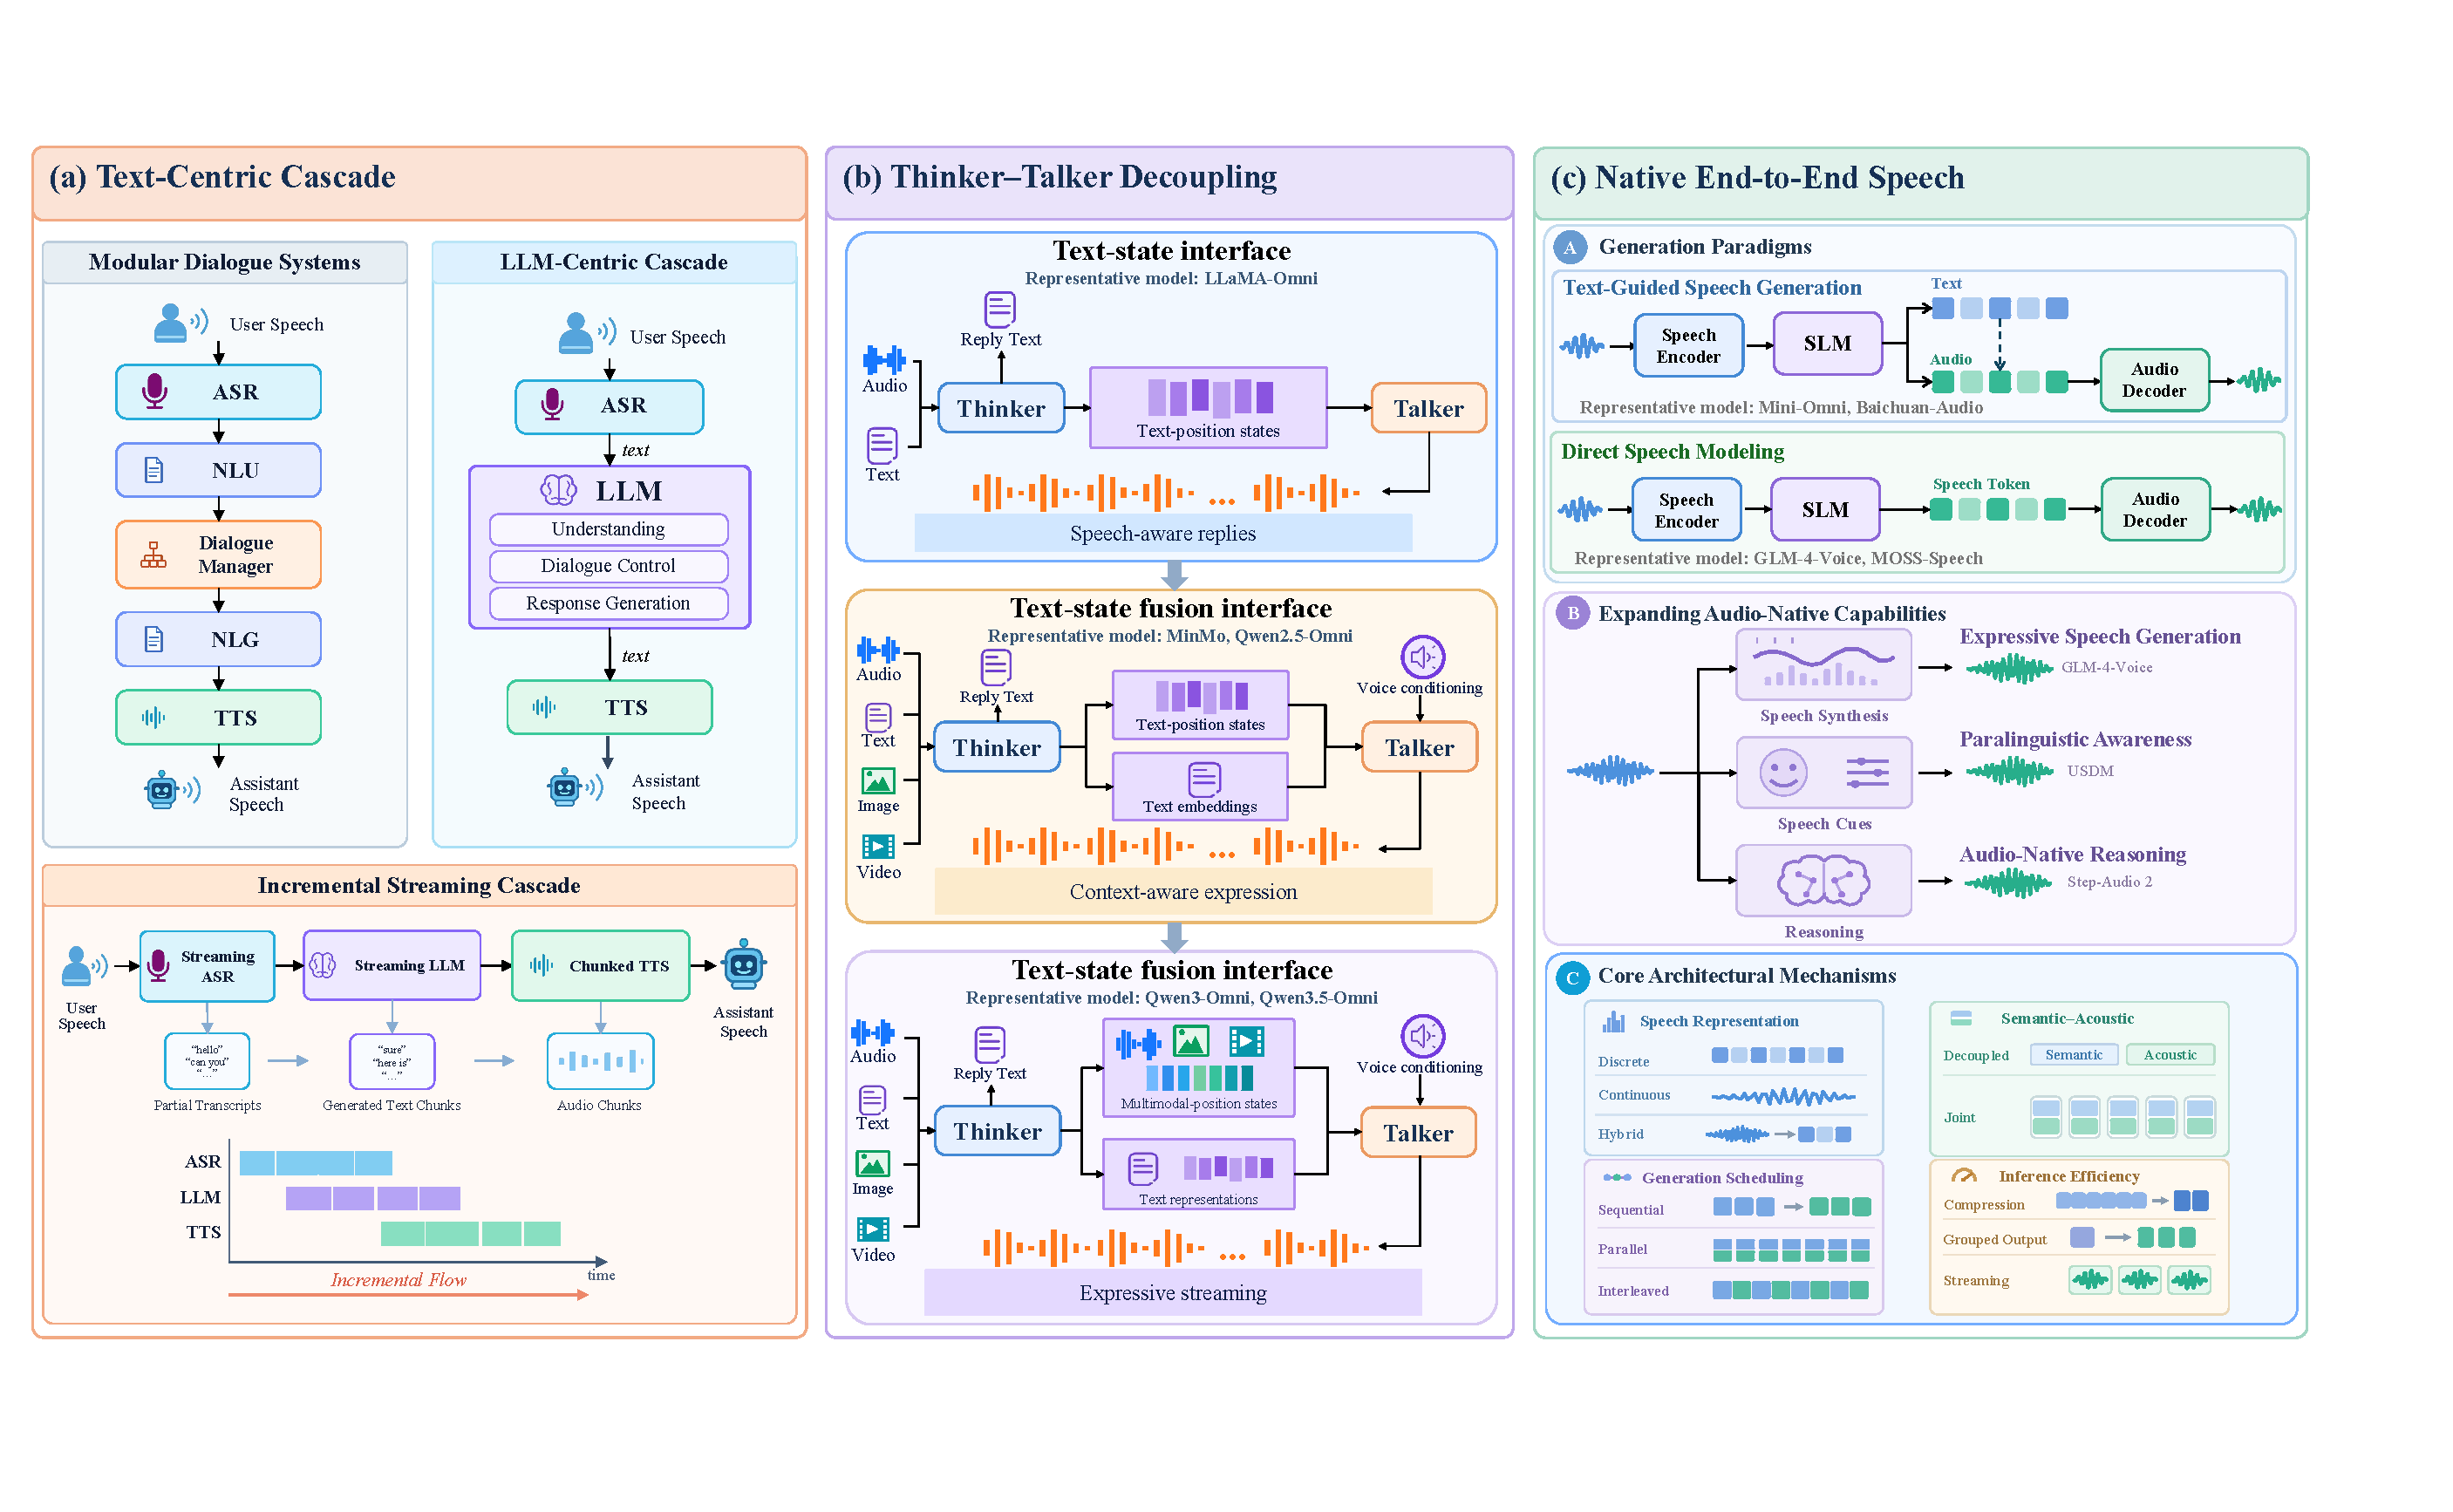
\includegraphics[width=\textwidth]{figures/half-duplex-overview.pdf}
    \caption{    
    Overview of half-duplex speech interaction architectures.
    (a) Text-centric cascaded interaction, comprising modular dialogue
    systems, LLM-centered cascades, and incremental streaming pipelines.
    (b) Thinker-Talker decoupled interaction with response-state
    conditioning (top), text-state fusion (middle), and multimodal-state
    sharing (bottom).
    (c) Native end-to-end speech interaction, comprising text-guided
    generation and direct speech modeling (top), audio-native capabilities
    (middle), and core architectural mechanisms (bottom).
    Streaming and overlapping computation operate within alternating
    conversational turns.
    }
    \label{fig:half-duplex-overview}
\end{figure}


\subsubsection{Text-Centric Cascaded Interaction}
\label{sec:text-centric-cascaded-interaction}

Text-centric cascaded interaction operates on the principle of mapping speech to textual counterparts for perception, reasoning, and generation. In this paradigm, text serves as the principal intermediary: recognition converts user speech into transcripts, from which the dialogue core interprets intentions, maintains context, and formulates a textual reply for synthesis~\citep{DBLP:journals/csur/McTear02,DBLP:journals/corr/abs-2411-13577}. Historically, the intermediate processing relied on highly fragmented pipelines, which have progressively evolved into more unified language backbones. The contemporary ASR $\rightarrow$ LLM $\rightarrow$ TTS architecture represents the current apex of this text-centric philosophy. In the half-duplex setting, users and systems alternate turns while internal processing can overlap. Figure~\ref{fig:half-duplex-overview}(a) traces this evolution,and Table~\ref{tab:half-duplex-systems} summarizes representative cascaded systems and related methods.

% % Required packages: booktabs, graphicx

\begin{table*}[t]
    \centering
    \caption{
        Text-centric cascaded systems and methods.
        \textit{Note.} SDS: spoken dialogue system.
        Interface identifies model-facing or inter-module representations;
        Execution highlights control and scheduling (``--'': outside scope).
        Text-only models provide language-side foundations;
        frameworks are compared through their cascaded paths.
        Streaming and internal overlap can operate within alternating turns.
    }
    \label{tab:text-centric-cascaded-comparison}
    \small
    \renewcommand{\arraystretch}{1.12}
    \setlength{\tabcolsep}{5pt}

    \resizebox{\textwidth}{!}{
    \begin{tabular}{l|l|l|l|l|l}
        \toprule
        \textbf{Work}
        & \textbf{Type}
        & \textbf{Interface}
        & \textbf{Language Core}
        & \textbf{Execution}
        & \textbf{Key Feature} \\
        \midrule

        \multicolumn{6}{l}{
            \textit{Modular systems and language-side consolidation}
        } \\
        \midrule

        GALAXY-II \citep{DBLP:conf/interspeech/SeneffHLPSZ98}
        & Architecture
        & Symbolic messages
        & Modular
        & Hub-controlled
        & Programmable distributed hub \\

        RavenClaw \citep{DBLP:journals/csl/BohusR09}
        & Framework
        & Symbolic representations
        & Modular
        & Task-driven
        & Task--skill separation \\

        POMDP SDS \citep{DBLP:journals/pieee/YoungGTW13}
        & Method
        & ASR/NLU hypotheses
        & Modular
        & Belief-driven
        & Uncertainty-aware control \\

        Wen et al. \citep{DBLP:conf/eacl/Rojas-BarahonaG17}
        & Model
        & Text
        & Neural TOD
        & --
        & Text-level end-to-end learning \\

        Sequicity \citep{DBLP:conf/acl/KanHLJRY18}
        & Model
        & Text
        & Seq2seq
        & --
        & Explicit belief span \\

        SimpleTOD \citep{DBLP:conf/nips/Hosseini-AslMWY20}
        & Model
        & Text
        & Causal LM
        & Autoregressive
        & State--action--response serialization \\

        SOLOIST \citep{DBLP:journals/tacl/PengLLSLG21}
        & Model
        & Text
        & Pretrained LM
        & Autoregressive
        & Transfer and machine teaching \\

        \midrule
        \multicolumn{6}{l}{
            \textit{Modern cascades and capability integration}
        } \\
        \midrule

        AudioGPT \citep{DBLP:conf/aaai/HuangLYSCYWHHLR24}
        & Agent
        & Text / tool calls
        & ChatGPT
        & Tool-orchestrated
        & External audio models \\

        ESPnet-SDS \citep{DBLP:conf/naacl/Arora0STCBFKTSS25}
        & Toolkit
        & Configurable
        & Configurable
        & Configurable
        & Cascade / E2E evaluation \\

        Eva \citep{DBLP:conf/ifaamas/QinZ25}
        & Agent
        & Text / tool calls
        & LLM
        & Agent-orchestrated
        & RAG, agents, telephony \\

        LiveKit Agents \citep{livekitagentsdocs}
        & Framework
        & Pipeline-dependent
        & Swappable
        & Configurable streaming
        & Pipeline / provider selection \\

        Pipecat \citep{pipecatdocs}
        & Framework
        & Frames
        & Swappable
        & Frame-streaming
        & Frame-based processors \\

        \midrule
        \multicolumn{6}{l}{
            \textit{Incremental processing and latency optimization}
        } \\
        \midrule

        Schlangen \& Skantze \citep{DBLP:journals/dad/SchlangenS11}
        & Method
        & Incremental units
        & Agnostic
        & Incremental
        & Revision and commitment \\

        InproTK \citep{DBLP:conf/naacl/BaumannS12}
        & Toolkit
        & Incremental units
        & Modular
        & Incremental
        & Reusable incremental modules \\

        Skantze \& Hjalmarsson \citep{DBLP:journals/csl/SkantzeH13}
        & Method
        & Incremental representations
        & Modular
        & Incremental
        & Planning and self-monitoring \\

        Telecom Agent \citep{DBLP:journals/corr/abs-2508-04721}
        & Agent
        & Text
        & 4-bit LLM
        & Concurrent
        & Domain ASR/TTS + RAG \\

        LTS-VoiceAgent \citep{DBLP:journals/corr/abs-2601-19952}
        & Agent
        & Partial text
        & LLM
        & Semantically triggered
        & \textit{When to think} \\

        DDTSR \citep{DBLP:journals/corr/abs-2602-23266}
        & Method
        & Streaming text
        & LLM
        & Cross-stage overlap
        & \textit{Speak while thinking} \\

        \bottomrule
    \end{tabular}
    }

\end{table*}


\paragraph{Textual representation and unified understanding.}
Textual representations support the interpretation of user utterances, the tracking of dialogue context, and the reasoning required for task execution. Classical systems distributed these responsibilities across distinct language understanding, dialogue management, and language generation modules~\citep{DBLP:journals/csur/McTear02}. POMDP-based managers maintained beliefs over uncertain recognition results and user intentions to guide dialogue decisions~\citep{DBLP:journals/pieee/YoungGTW13}. Neural models subsequently brought these functions into shared modeling: SimpleTOD, for instance, serialized belief states, dialogue actions, and responses within a single causal language model~\citep{DBLP:conf/nips/Hosseini-AslMWY20}. Modern LLM-centered systems further consolidate contextual interpretation, response generation, and tool orchestration, exemplified by AudioGPT's use of ChatGPT to coordinate external audio models~\citep{DBLP:conf/aaai/HuangLYSCYWHHLR24}. Consequently, while language-side processing has become highly unified, it continues to rely on text transcripts to represent the user's spoken input.

\paragraph{Response modeling and the text bottleneck.}
Reply formation connects the interpreted request and dialogue context to a response decision, its verbal formulation, and its spoken realization. While modular systems separate dialogue policy from language generation, shared autoregressive models now jointly generate dialogue actions and condition reply text on them~\citep{DBLP:journals/csur/McTear02,DBLP:conf/nips/Hosseini-AslMWY20}. The resulting text carries the lexical content to the TTS module. However, relying solely on text creates an inherent bottleneck with two major gaps: input transcripts incompletely preserve vocal cues (e.g., emotion, intonation) relevant to deciding \textit{how} to respond, and output text underspecifies the intended prosody and speaking style for synthesis~\citep{DBLP:conf/acl/CuiYJMZWGK25}. FireRedChat illustrates the input boundary through its text-only cascaded LLM and its audio-aware semi-cascaded alternative~\citep{chen2025fireredchat}. Auxiliary descriptions can partly bridge these gaps; for example, X-Talk injects acoustic descriptions into the LLM's system prompt and allows the adjustment of TTS emotion vectors~\citep{DBLP:journals/corr/abs-2512-18706}. Nevertheless, their coverage remains bounded by what analysis modules can extract and synthesis controls can express, meaning text-mediated coordination inherently limits the preservation of rich acoustic information.

\paragraph{Component optimization and interface coordination.}
Explicit textual interfaces allow recognition, dialogue processing, and synthesis to be trained, evaluated, adapted, or replaced independently. ESPnet-SDS supports configurable pipelines and rigorous component evaluation~\citep{DBLP:conf/naacl/Arora0STCBFKTSS25}; Eva integrates telephony, retrieval, and task agents around a speech dialogue pipeline~\citep{DBLP:conf/ifaamas/QinZ25}; and LiveKit Agents exposes interchangeable speech and language providers for developers~\citep{livekitagentsdocs}. Such modularity supports extensive reuse and application-specific adaptation, but it requires connected components to exchange compatible information. Coordination can also be learned locally to smooth the interfaces: DDTSR trains a lightweight connective model to ensure continuity with subsequent large-model replies, progressively adapting it to partial inputs~\citep{DBLP:journals/corr/abs-2602-23266}. Independent component improvements therefore necessitate interface-level checks, as recognition errors can cascade to alter downstream decisions, and a semantically correct reply still requires suitable formatting for its intended vocal delivery.

\paragraph{Streaming execution and output commitment.}
Waiting for complete transcripts and full LLM replies creates latency barriers between perception, response formation, and synthesis. Incremental execution addresses this by letting downstream stages process partial results. Schlangen and Skantze formalized this through revisable and committed hypotheses~\citep{DBLP:journals/dad/SchlangenS11}, while frameworks like Pipecat implement streaming orchestration via frame processors~\citep{pipecatdocs}. Scheduling mechanisms must decide when to trigger reasoning and when to synthesize available text. LTS-VoiceAgent triggers reasoning from informative speech prefixes~\citep{DBLP:journals/corr/abs-2601-19952}, and DDTSR prepares short connectives from partial transcripts while a larger model computes the substantive reply~\citep{DBLP:journals/corr/abs-2602-23266}. However, earlier execution introduces revision costs: changing transcripts can invalidate speculative replies, and already-played speech requires conversational repair. Hypothesis revision, cancellation, and output commitment therefore govern the delicate balance between responsiveness and stability~\citep{DBLP:journals/dad/SchlangenS11}. Consequently, evaluation must distinguish \textit{time to first audio} from \textit{time to substantive response}, as early connectives can advance the onset without delivering the actual answer~\citep{DBLP:journals/corr/abs-2602-23266}. 

Ultimately, while incremental execution mitigates latency, cascaded systems remain constrained by their text-centric architecture. Relying on transcripts loses rich vocal cues, risks cascading errors, and forces complex trade-offs between responsiveness and revision costs. To bypass this text bottleneck, Thinker-Talker systems evolve the paradigm by bringing continuous speech representations directly into the understanding backbone.

\subsubsection{Thinker-Talker Decoupled Interaction}
\label{sec:thinker-talker-decoupled-interaction}
Thinker-Talker interaction centers on an audio understanding model that directly receives continuous speech representations and formulates its response as text. The Thinker retains language capabilities for semantic understanding and deep reasoning over audio and dialogue history, while the Talker can use its hidden states and text conditions for streaming speech after turn handover~\citep{DBLP:journals/corr/abs-2501-06282,DBLP:journals/corr/abs-2503-20215,DBLP:journals/corr/abs-2509-17765}. Their decoupled optimization combines understanding depth with generation efficiency~\citep{DBLP:conf/icml/WangLFZS000M25}. This paradigm has become a mainstream approach to optimizing end-to-end half-duplex speech interaction~\citep{DBLP:conf/iclr/FangGZMZ025,DBLP:journals/corr/abs-2501-06282,DBLP:journals/corr/abs-2503-20215,DBLP:journals/corr/abs-2509-17765}. Figure~\ref{fig:half-duplex-overview}(b) illustrates the evolution
of Thinker-Talker information sharing, and
Table~\ref{tab:half-duplex-systems} summarizes representative
systems and their architectural highlights.

\paragraph{Continuous speech representations for language understanding.}
The Thinker's input interface aligns continuous audio encoder features
with a pretrained language backbone to support speech understanding
and text response formulation~\citep{DBLP:conf/iclr/FangGZMZ025,DBLP:journals/corr/abs-2501-06282,DBLP:journals/corr/abs-2503-20215}.
LLaMA-Omni uses a speech adapter~\citep{DBLP:conf/iclr/FangGZMZ025},
while MinMo employs input alignment to convey speech content,
emotion, and audio events~\citep{DBLP:journals/corr/abs-2501-06282}.
Uni-MoE combines audio and speech connectors with modality-specific
experts and progressive training for multimodal
understanding~\citep{DBLP:journals/pami/LiJHWZLMZ25}.
This alignment must preserve vocal cues and environmental sounds
that transcripts may lose so that they can inform language understanding,
reasoning, and response formulation.
When supported, incremental encoding begins as speech arrives;
in the half-duplex setting, spoken replies follow turn handover.

\paragraph{Hidden-state and text conditioning for speech generation.}
As the Thinker formulates a response, the interface must convey its lexical content to the Talker while retaining information relevant to spoken delivery. These interfaces differ in whether lexical content is carried
implicitly by internal representations or supplied explicitly as text,
with representative conditioning mechanisms summarized in
Table~\ref{tab:half-duplex-systems}.
LLaMA-Omni carries lexical content implicitly through response
hidden states~\citep{DBLP:conf/iclr/FangGZMZ025}, while other designs combine
text tokens or embeddings with internal representations through
prefix conditioning, projection, or fusion~\citep{DBLP:conf/icml/WangLFZS000M25,DBLP:journals/corr/abs-2501-06282,DBLP:journals/corr/abs-2503-20215,DBLP:journals/corr/abs-2505-02625}.
Beyond lexical content, shared representations allow user audio and
dialogue history to guide spoken delivery, while explicit voice
conditions provide additional control.
MinMo and Qwen2.5-Omni share user-query and dialogue-history
information~\citep{DBLP:journals/corr/abs-2501-06282,DBLP:journals/corr/abs-2503-20215}, while Qwen3-Omni
and Qwen3.5-Omni supply multimodal Thinker representations with
historical and streaming text; the latter also provides voice
conditions~\citep{DBLP:journals/corr/abs-2509-17765,DBLP:journals/corr/abs-2604-15804}.
Uni-MoE-2.0-Omni uses explicit conditioning, conveying response text and voice-control
prompts to a separate context-aware MoE-TTS
module~\citep{DBLP:journals/corr/abs-2511-12609}.
Effective transfer of these conditions helps the Talker
preserve response wording and adapt emphasis and affect to the
dialogue context, supporting consistency between semantic content
and acoustic expression.

% \begin{table}[t]
    \centering
    \caption{Thinker-Talker systems in turn-based speech dialogue: continuous audio inputs and text replies. Visual encoders indicate additional capabilities. AR/NAR: autoregressive/non-autoregressive; CTC: connectionist temporal classification; KV: key/value; MTP: multi-token prediction; AuT: Audio Transformer; TMRoPE: time-aligned multimodal rotary position embedding; ARIA: Adaptive Rate Interleave Alignment.}
    \label{tab:thinker-talker}
    \small
    \setlength{\tabcolsep}{4pt}
    \renewcommand{\arraystretch}{1.1}
    \begin{tabular}{@{}>{\raggedright\arraybackslash}p{\dimexpr0.18\linewidth-6pt\relax}>{\raggedright\arraybackslash}p{\dimexpr0.26\linewidth-6pt\relax}>{\raggedright\arraybackslash}p{\dimexpr0.29\linewidth-6pt\relax}>{\raggedright\arraybackslash}p{\dimexpr0.27\linewidth-6pt\relax}@{}}
        \toprule
        \textbf{System} & \textbf{Thinker}\newline Input / understanding & \textbf{Interface}\newline Talker conditions & \textbf{Talker}\newline Generation / streaming \\
        \midrule
        LLaMA-Omni\newline\citep{DBLP:conf/iclr/FangGZMZ025} & Whisper + adapter;\newline speech instructions & Response hidden states;\newline no separate text input & NAR/CTC units;\newline chunked vocoding \\
        \addlinespace
        Freeze-Omni\newline\citep{DBLP:conf/icml/WangLFZS000M25} & Streaming encoder + adapter; frozen LLM & Text tokens +\newline hidden-state prefix KV & NAR prefill + AR tokens;\newline streaming codec \\
        \addlinespace
        MinMo\newline\citep{DBLP:journals/corr/abs-2501-06282} & SenseVoice + projector;\newline speech, emotion, events & Text embeddings + query/response states; projection & AR tokens; fixed interleaving;\newline chunked flow matching \\
        \addlinespace
        Qwen2.5-Omni\newline\citep{DBLP:journals/corr/abs-2503-20215} & Audio/vision encoders;\newline TMRoPE alignment & Text embeddings + Thinker states; shared history & Dual-track AR;\newline sliding-window flow matching \\
        \addlinespace
        LLaMA-Omni~2\newline\citep{DBLP:journals/corr/abs-2505-02625} & Whisper + adapter;\newline multi-turn adaptation & Text embeddings + response states; gated fusion & AR read/write scheduling;\newline causal flow matching \\
        \addlinespace
        Qwen3-Omni\newline\citep{DBLP:journals/corr/abs-2509-17765} & AuT + vision encoder;\newline temporal-ID alignment & Historical/streaming text + multimodal states & AR + residual-codebook MTP;\newline causal ConvNet \\
        \addlinespace
        \mbox{Uni-MoE-2.0-Omni}\newline\citep{DBLP:journals/corr/abs-2511-12609}
        & Whisper/Q-Former + vision encoder;\newline 3D RoPE alignment
        & Text tokens + voice-control prompts
        & AR tokens; sentence-level streaming;\newline WavTokenizer decoding \\
        \addlinespace
        Qwen3.5-Omni\newline\citep{DBLP:journals/corr/abs-2604-15804} & AuT + vision encoder;\newline explicit timestamps & Historical/streaming text + multimodal states; voice prompt & ARIA interleaving;\newline multi-codebook prediction;\newline causal ConvNet \\
        \bottomrule
    \end{tabular}
\end{table}


\paragraph{Decoupled training and cross-module alignment.}
Decoupled training coordinates language and acoustic objectives while retaining the Thinker's language capabilities. On the understanding side, adaptation strategies differ in which components receive updates: the language backbone can remain frozen, as in Freeze-Omni, or be updated with the input adapter while the speech encoder stays frozen, as in LLaMA-Omni and LLaMA-Omni~2~\citep{DBLP:conf/icml/WangLFZS000M25,DBLP:conf/iclr/FangGZMZ025,DBLP:journals/corr/abs-2505-02625}. MinMo combines progressive input alignment with low-rank adaptation (LoRA) of the LLM, while the Qwen series unfreezes the language backbone during staged multimodal pretraining~\citep{DBLP:journals/corr/abs-2501-06282,DBLP:journals/corr/abs-2503-20215,DBLP:journals/corr/abs-2509-17765,DBLP:journals/corr/abs-2604-15804}. On the generation side, training aligns the interface and speech generator with the resulting representations. With the understanding side frozen, updates can be confined to a speech decoder or an added prefix decoder, as in LLaMA-Omni and Freeze-Omni, respectively~\citep{DBLP:conf/iclr/FangGZMZ025,DBLP:conf/icml/WangLFZS000M25}. Local joint optimization couples the interface with speech prediction: LLaMA-Omni~2 and MinMo jointly train their respective gate fusion module and output projector with the speech generation model~\citep{DBLP:journals/corr/abs-2505-02625,DBLP:journals/corr/abs-2501-06282}. Across both modules, the Qwen series uses specialized post-training for instruction following and reasoning in the Thinker, and contextual generation, preference alignment, and speaker control in the Talker~\citep{DBLP:journals/corr/abs-2503-20215,DBLP:journals/corr/abs-2509-17765,DBLP:journals/corr/abs-2604-15804}. These schedules aim to preserve response quality while aligning spoken content and expression with the intended answer.

\paragraph{Incremental speech prediction and streaming synthesis.}
After turn handover, timely and fluent spoken replies require coordination between text-derived conditions, speech-unit prediction, and waveform synthesis. Waiting for more text supplies context for pronunciation and prosody, while smaller increments support earlier playback. Incremental prediction and interleaved scheduling address this trade-off, with representative mechanisms summarized in Table~\ref{tab:half-duplex-systems}. Speech units can be emitted from incoming response hidden states using non-autoregressive prediction, as in LLaMA-Omni's decoder trained with connectionist temporal classification (CTC)~\citep{DBLP:conf/iclr/FangGZMZ025}. Autoregressive generation can instead interleave the consumption of text-derived conditions with speech prediction, as in MinMo~\citep{DBLP:journals/corr/abs-2501-06282}. Coordinating the different text and speech token rates is a further scheduling concern, addressed by Qwen3.5-Omni's Adaptive Rate Interleave Alignment (ARIA)~\citep{DBLP:journals/corr/abs-2604-15804}. Waveform synthesis then converts predicted units into playable segments through chunk-aware flow matching, as in CosyVoice~2 used by MinMo~\citep{DBLP:journals/corr/abs-2412-10117}, or causal convolutional decoding, as in Qwen3-Omni~\citep{DBLP:journals/corr/abs-2509-17765}. Together, incremental prediction and streaming synthesis shape how soon users hear the reply and how smoothly it continues, with generation scheduling governing the availability of speech units and synthesis throughput and chunk transitions affecting playback continuity.

Overall, Thinker-Talker interaction uses direct speech understanding and hidden-state sharing to make replies more contextually appropriate and spoken expression better aligned with intent. These gains depend on cross-module alignment and coordinated streaming for consistent, fluent delivery. While the Thinker organizes replies as text, native end-to-end interaction brings speech representations into both the input and output modeling of the dialogue backbone.


% Required packages: booktabs, array, tabularx

\begin{table*}[!tp]
    \centering
    \caption{
        Representative systems and methods for half-duplex speech interaction.
        SDS: spoken dialogue system; TOD: task-oriented dialogue;
        CTC: connectionist temporal classification;
        ARIA: Adaptive Rate Interleave Alignment.
        FireRedChat is shown in its cascaded configuration.
    }
    \label{tab:half-duplex-systems}
    \scriptsize
    \setlength{\tabcolsep}{3pt}
    \renewcommand{\arraystretch}{1.3}

    \begin{tabularx}{\textwidth}{
        @{}
        >{\raggedright\arraybackslash}p{0.25\textwidth}
        >{\raggedright\arraybackslash}p{0.13\textwidth}
        >{\raggedright\arraybackslash}p{0.24\textwidth}
        >{\raggedright\arraybackslash}X
        @{}
    }
        \toprule
        \textbf{System / Work}
        & \textbf{Architecture}
        & \textbf{Input / Output}
        & \textbf{Highlight} \\
        \midrule

        \multicolumn{4}{@{}l}{\textit{Text-centric cascaded systems and methods}} \\
        \midrule

        GALAXY-II~\citep{DBLP:conf/interspeech/SeneffHLPSZ98}
        & Modular SDS & Speech / Speech
        & Programmable hub for distributed modules \\

        POMDP SDS~\citep{DBLP:journals/pieee/YoungGTW13}
        & Modular SDS & Speech / Speech
        & Belief-state dialogue control \\

        SimpleTOD~\citep{DBLP:conf/nips/Hosseini-AslMWY20}
        & Text-only TOD & Text / Text
        & State--action--response serialization \\

        AudioGPT~\citep{DBLP:conf/aaai/HuangLYSCYWHHLR24}
        & Cascade & Text, Audio, Image, Score / Text, Audio, Video
        & LLM orchestration of audio tools \\

        ESPnet-SDS~\citep{DBLP:conf/naacl/Arora0STCBFKTSS25}
        & Configurable & Configurable
        & Cascade and end-to-end evaluation \\

        Eva~\citep{DBLP:conf/ifaamas/QinZ25}
        & Cascade & Speech / Speech
        & Retrieval and telephony integration \\

        LiveKit Agents~\citep{livekitagentsdocs}
        & Configurable & Pipeline-dependent
        & Interchangeable speech and language providers \\

        Pipecat~\citep{pipecatdocs}
        & Configurable & Pipeline-dependent
        & Frame-based streaming processors \\

        Schlangen \& Skantze~\citep{DBLP:journals/dad/SchlangenS11}
        & Modular & Modality-agnostic
        & Incremental units with revision and commitment \\

        InproTK~\citep{DBLP:conf/naacl/BaumannS12}
        & Modular & Configurable
        & Reusable incremental processing modules \\

        Telecom Agent~\citep{DBLP:journals/corr/abs-2508-04721}
        & Cascade & Speech / Speech
        & Domain ASR/TTS; concurrent execution \\

        FireRedChat~\citep{DBLP:journals/corr/abs-2509-06502}
        & Cascade & Speech / Text, Speech
        & Pluggable cascade; streaming synthesis \\

        LTS-VoiceAgent~\citep{DBLP:journals/corr/abs-2601-19952}
        & Cascade & Speech / Text
        & Speech-prefix triggers for reasoning \\

        DDTSR~\citep{DBLP:journals/corr/abs-2602-23266}
        & Cascade & Speech / Speech
        & Early connectives; cross-stage overlap \\

        \midrule
        \multicolumn{4}{@{}l}{\textit{Thinker-Talker decoupled systems}} \\
        \midrule

        LLaMA-Omni~\citep{DBLP:conf/iclr/FangGZMZ025}
        & Thinker-Talker & Speech / Text, Speech
        & Response states; CTC decoding \\

        Freeze-Omni~\citep{DBLP:conf/icml/WangLFZS000M25}
        & Thinker-Talker & Text, Speech / Text, Speech
        & Frozen LLM; hidden-state prefix \\

        MinMo~\citep{DBLP:journals/corr/abs-2501-06282}
        & Thinker-Talker & Text, Audio / Text, Speech
        & Text and context states; interleaving \\

        Qwen2.5-Omni~\citep{DBLP:journals/corr/abs-2503-20215}
        & Thinker-Talker & Text, Audio, Image, Video / Text, Speech
        & Shared Thinker states; dual-track decoding \\

        LLaMA-Omni~2~\citep{DBLP:journals/corr/abs-2505-02625}
        & Thinker-Talker & Speech / Text, Speech
        & Gated fusion; read/write scheduling \\

        Qwen3-Omni~\citep{DBLP:journals/corr/abs-2509-17765}
        & Thinker-Talker & Text, Audio, Image, Video / Text, Speech
        & Multimodal states; causal decoding \\

        Uni-MoE-2.0-Omni~\citep{DBLP:journals/corr/abs-2511-12609}
        & Thinker-Talker & Text, Audio, Image, Video / Text, Speech, Image
        & Text and voice prompts for MoE-TTS \\

        Qwen3.5-Omni~\citep{DBLP:journals/corr/abs-2604-15804}
        & Thinker-Talker & Text, Audio, Image, Video / Text, Speech
        & Multimodal and voice conditions; ARIA \\

        \midrule
        \multicolumn{4}{@{}l}{\textit{Native end-to-end speech systems}} \\
        \midrule

        SpeechGPT~\citep{DBLP:conf/emnlp/ZhangLZZWZQ23}
        & Native Speech & Text, Speech / Text, Speech
        & Discrete units; cross-modal tuning \\

        USDM~\citep{DBLP:conf/nips/KimSJKKKLSOHYY24}
        & Native Speech & Text, Speech / Text, Speech
        & Speech-text pretraining; prosody cues \\

        Mini-Omni~\citep{DBLP:journals/corr/abs-2408-16725}
        & Native Speech & Text, Speech / Text, Speech
        & Parallel text and audio generation \\

        IntrinsicVoice~\citep{DBLP:journals/corr/abs-2410-08035}
        & Native Speech & Text, Speech / Text, Speech
        & GroupFormer speech compression \\

        GLM-4-Voice~\citep{DBLP:journals/corr/abs-2412-02612}
        & Native Speech & Text, Speech / Text, Speech
        & Low-rate tokens; streaming decoding \\

        Flow-Omni~\citep{DBLP:journals/corr/abs-2412-04917}
        & Native Speech & Text, Speech / Text, Speech
        & Continuous speech via flow matching \\

        SLAM-Omni~\citep{DBLP:conf/acl/Chen0YLLXN00L0025}
        & Native Speech & Speech / Text, Speech
        & Grouped semantic tokens; vocoder \\

        Baichuan-Audio~\citep{DBLP:journals/corr/abs-2502-17239}
        & Native Speech & Text, Audio / Text, Speech
        & Joint semantic-acoustic codebooks \\

        Kimi-Audio~\citep{DBLP:journals/corr/abs-2504-18425}
        & Native Speech & Text, Audio / Text, Speech
        & Continuous inputs; discrete outputs \\

        VITA-Audio~\citep{DBLP:journals/corr/abs-2505-03739}
        & Native Speech & Text, Speech / Text, Speech
        & Multi-token audio prediction \\

        Step-Audio~2~\citep{DBLP:journals/corr/abs-2507-16632}
        & Native Speech & Text, Audio / Text, Speech
        & Audio-native reasoning with RL \\

        MOSS-Speech~\citep{DBLP:conf/iclr/ZhaoXJWCJCLCWZC26}
        & Native Speech & Speech / Speech
        & Modality-specific layers; no text guidance \\

        GPT-Realtime-2.1~\citep{openai2026gptrealtime21}
        & Native Speech & Text, Audio, Image / Text, Speech
        & Speech reasoning and tool calling \\

        Qwen-Audio~3.1+~\citep{alibaba2026qwenaudio31realtime}
        & Native Speech & Text, Audio / Text, Speech
        & Push-to-talk with function calling \\

        EVI~3~\citep{cowen2025evi3}
        & Native Speech & Text, Speech / Text, Speech
        & Coordinated content and prosody \\

        \bottomrule
    \end{tabularx}
\end{table*}

\subsubsection{Native End-to-End Speech Interaction}
\label{sec:native-end-to-end-speech-interaction}
Native end-to-end speech interaction uses a dialogue backbone that models speech representations on both the input and output paths: a speech language model sits between a speech encoder or tokenizer and a speech decoder, so that a turn proceeds as speech $\rightarrow$ speech representation $\rightarrow$ speech language model $\rightarrow$ speech representation $\rightarrow$ speech. Semantic content, prosody, emotion, and speaker characteristics can then inform the reply to the extent that the representations retain them. In the half-duplex setting, input may be encoded incrementally and response speech streams after turn handover; continuous listening and interruption during system speech belong to full-duplex interaction. Figure~\ref{fig:half-duplex-overview}(c) summarizes generation paradigms (A), audio-native capabilities (B), and core architectural mechanisms (C).

\paragraph{Discrete, continuous, and hybrid speech representations in the backbone.}
The paradigm originates in speech language modeling: GSLM modeled discrete self-supervised units with language-model objectives~\citep{lakhotia2021gslm}, and SpeechGPT brought such units into a pretrained text LLM that both receives and emits speech~\citep{DBLP:conf/emnlp/ZhangLZZWZQ23}. Representations first differ in form. Discrete tokens let speech reuse next-token prediction, as in GLM-4-Voice's low-rate single-codebook tokens~\citep{DBLP:journals/corr/abs-2412-02612}; Flow-Omni models continuous speech features alongside discrete text and generates speech through flow matching~\citep{DBLP:journals/corr/abs-2412-04917}; and Kimi-Audio pairs continuous inputs for understanding with discrete outputs for generation~\citep{DBLP:journals/corr/abs-2504-18425}. They also differ in whether semantic and acoustic information are decoupled or modeled jointly: SLAM-Omni predicts compact semantic tokens and leaves timbre and acoustic realization to the vocoder~\citep{DBLP:conf/acl/Chen0YLLXN00L0025}, whereas Baichuan-Audio keeps both in a multi-codebook representation~\citep{DBLP:journals/corr/abs-2502-17239}. Continuous or hybrid inputs retain more vocal cues for understanding, while discrete outputs keep generation within token prediction; decoupling shortens backbone sequences and eases alignment with text but leaves expressive detail to the decoder, whereas joint modeling keeps that detail in the backbone at the cost of longer sequences.

\paragraph{Text-guided generation, direct speech modeling, and vocal cues in response planning.}
The two generation paradigms differ in whether intermediate text guides what the reply says. Text-guided generation conditions audio on text from the same backbone, whether the text precedes speech units, as in SpeechGPT and USDM~\citep{DBLP:conf/emnlp/ZhangLZZWZQ23,DBLP:conf/nips/KimSJKKKLSOHYY24}, serves as a semantic channel that instructs audio generation, as in Mini-Omni~\citep{DBLP:journals/corr/abs-2408-16725}, or is interleaved with audio tokens to anchor content, as in Baichuan-Audio~\citep{DBLP:journals/corr/abs-2502-17239}. Direct speech modeling instead has the backbone predict speech tokens as its own output, as in GLM-4-Voice~\citep{DBLP:journals/corr/abs-2412-02612}; IntrinsicVoice reduces reliance on explicit text generation~\citep{DBLP:journals/corr/abs-2410-08035}, and MOSS-Speech removes text guidance through modality-based layer splitting~\citep{DBLP:conf/iclr/ZhaoXJWCJCLCWZC26}. Beyond content, native modeling moves vocal cues from rendering into planning: GLM-4-Voice shapes output prosody and style, USDM lets input prosody inform the reply, and Step-Audio~2's audio-native reasoning lets speaking style and emotion inform response behavior as well as voice~\citep{DBLP:journals/corr/abs-2507-16632}. Production systems combine these capabilities with reasoning and tool calling in GPT Realtime~2.1~\citep{openai2026gptrealtime21}, coordinated content and prosody in EVI~3~\citep{cowen2025evi3}, and function calling alongside a turn-based push-to-talk path in Qwen Audio~3.1 Realtime Plus~\citep{alibaba2026qwenaudio31realtime}. Text guidance stabilizes content through the backbone's language ability but limits expression to what text carries; direct modeling frees expression at the risk of weaker content control.

\paragraph{Unified pretraining, instruction tuning, freezing strategies, and reinforcement learning.}
Optimization must add speech modeling while retaining language capability; systems differ in which components are updated. SpeechGPT established modality-adaptation pretraining followed by cross-modal and chain-of-modality instruction tuning~\citep{DBLP:conf/emnlp/ZhangLZZWZQ23}. Later systems scale pretraining: USDM pretrains on unified speech-text sequences~\citep{DBLP:conf/nips/KimSJKKKLSOHYY24}, GLM-4-Voice and Baichuan-Audio pretrain on large-scale interleaved speech-text data before dialogue fine-tuning~\citep{DBLP:journals/corr/abs-2412-02612,DBLP:journals/corr/abs-2502-17239}, and Kimi-Audio pretrains jointly on audio and text before supervised fine-tuning~\citep{DBLP:journals/corr/abs-2504-18425}. Freezing strategies protect language ability at lower cost, as when Mini-Omni freezes the language model while aligning audio adapters~\citep{DBLP:journals/corr/abs-2408-16725} and MOSS-Speech trains added speech layers with the text layers frozen~\citep{DBLP:conf/iclr/ZhaoXJWCJCLCWZC26}. Reinforcement learning then shapes behavior beyond likelihood objectives, as in Step-Audio~2~\citep{DBLP:journals/corr/abs-2507-16632}. Interleaved pretraining aligns the modalities deeply but is expensive; freezing preserves text capability at the risk of weaker speech-text coordination, on which semantic-acoustic consistency depends.

\paragraph{Sequence compression, multi-token prediction, and streaming decoding.}
Speech sequences are far longer than text, so execution mechanisms govern startup latency and playback continuity. Compression shortens the sequence, through low-rate tokenization in GLM-4-Voice or GroupFormer's text-comparable lengths in IntrinsicVoice~\citep{DBLP:journals/corr/abs-2412-02612,DBLP:journals/corr/abs-2410-08035}, and grouped output reduces decoding steps, as SLAM-Omni predicts a group of semantic tokens per step~\citep{DBLP:conf/acl/Chen0YLLXN00L0025} and VITA-Audio's Multiple Cross-modal Token Prediction emits several audio tokens per forward pass~\citep{DBLP:journals/corr/abs-2505-03739}. Scheduling, independently of text guidance, determines when speech can begin: SpeechGPT and USDM complete the text first, Mini-Omni generates text and audio tokens in parallel, and GLM-4-Voice and Baichuan-Audio interleave them so that speech starts after a few text tokens. Streaming decoding then turns tokens into playable chunks, as in GLM-4-Voice's streaming flow-matching decoder and Kimi-Audio's chunk-wise detokenizer~\citep{DBLP:journals/corr/abs-2504-18425}. Parallel and interleaved schedules shorten waiting but require that speech not outrun the content it depends on, and stalls at chunk boundaries disrupt playback.

Native modeling brings vocal cues into both understanding and generation without a text bottleneck, at costs that follow the mechanisms above: compactness against acoustic detail, content stability against expressive freedom, language retention against modality alignment, and sequence length against latency. Interaction nonetheless remains organized around alternating turns, so half-duplex operation is defined by turn structure rather than by streaming capability.


\begin{TakeawayBox}{Takeaways: Half-Duplex Speech Interaction}
Half-duplex interaction progresses from text-mediated cascades to direct speech understanding with text-organized replies, then to native modeling of speech inputs and outputs. As speech representations take a greater role in this progression, vocal cues can more directly inform reply content and expression. These gains depend on representation quality and alignment, while generation scheduling shapes waiting time and playback continuity. Interaction remains organized around alternating turns.
\end{TakeawayBox}


% Section 3.3. Translated paragraph by paragraph from the updated Word source.
\subsection{Full-Duplex Speech Interaction}\label{sec:full-duplex}

% Word paragraph 1
Full-duplex speech interaction extends half-duplex turn-based interaction to concurrent behaviors such as simultaneous listening and speaking, interruption and floor-taking, and backchanneling. Conversational timing control consequently becomes central to interaction intelligence. According to the depth of coupling between timing control and the language-model backbone, this section distinguishes three paradigms: module-level external control, semi-embedded semantic assistance, and native dynamic interaction. These paradigms represent progressively tighter coupling between timing control and the backbone. Their mechanisms are examined in terms of timing-decision formation and streaming execution (Figure~\ref{fig:fullduplex}).

% Word paragraph 3; the original figure is preserved.
\begin{figure}[!htbp]
\centering
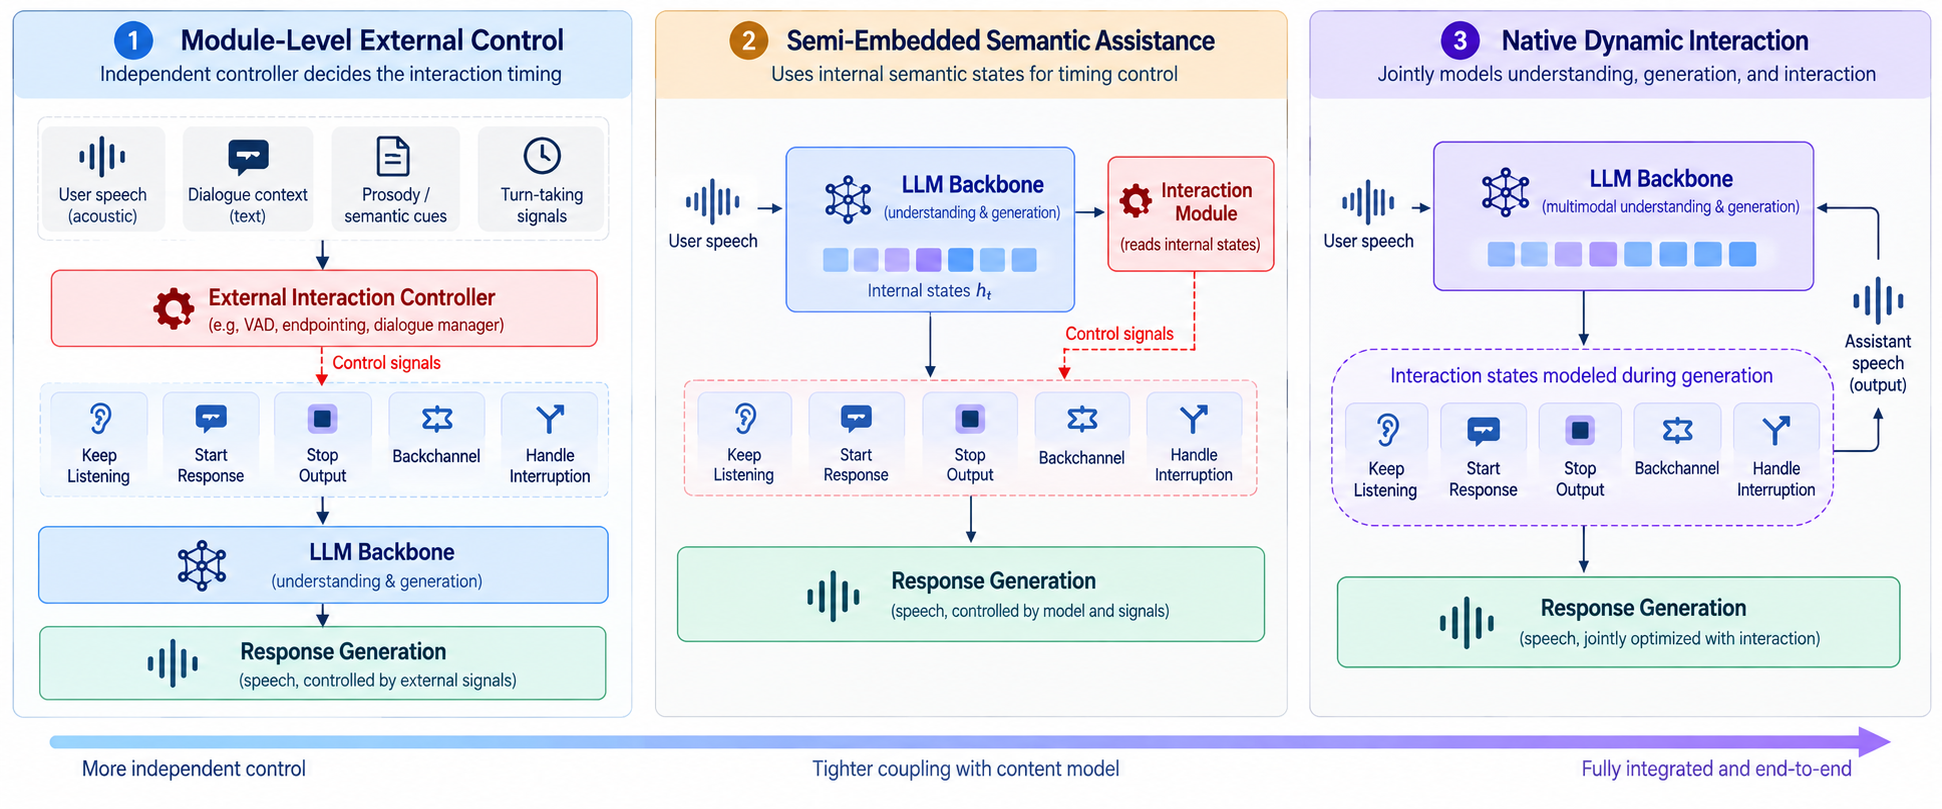
\includegraphics[width=\linewidth]{figures/fullduplex}
\caption{Three paradigms for coupling conversational timing control with the language-model backbone. From left to right: module-level external control, semi-embedded semantic assistance, and native dynamic interaction. The figure illustrates the control paths and execution interfaces of the three paradigms.}
\label{fig:fullduplex}
\end{figure}

% Word paragraph 4
\subsubsection{Module-Level External Control}\label{sec:fd-external}

% Word paragraph 5
Module-level external control places conversational timing control outside the language-model backbone. Independent external components, such as voice activity detection, endpoint detection, and dialogue management, make full-duplex interaction decisions and regulate input admission and response execution through explicit interfaces. Within this paradigm, the language model generates replies from admitted input and dialogue context, while an external controller schedules turn transitions, interruption handling, and backchannel initiation. This organization allows existing half-duplex backends to be reused when extending a system to full-duplex interaction.

% Word paragraphs 6--7
\paragraph{Evidence and state prediction for timing control.}
External timing control combines evidence of utterance completion with conditions for taking the floor. Dialogue context provides evidence of semantic completion, which TurnGPT uses to predict turn endings~\citep{DBLP:journals/corr/abs-2010-10874}. RC-TurnGPT adds a candidate response, extending the judgment to whether taking the floor is appropriate~\citep{DBLP:conf/acl/JiangES23}. Speech timing provides complementary evidence about how vocal activity may unfold: VAP projects future voice activity~\citep{DBLP:conf/interspeech/EkstedtS22}, while Next-Turn uses time-to-next-speech-onset supervision for streaming endpoint detection~\citep{DBLP:journals/corr/abs-2606-18094}. To guide execution, the controller maps these cues to states or actions. Joint modeling connects perception with state estimation. FlexDuo combines audio, dialogue history, and the previous state to predict Speak, Listen, and Idle actions~\citep{DBLP:journals/corr/abs-2502-13472}; SoulX-Duplug jointly predicts streaming ASR text and user states within an independent controller~\citep{arXiv:2603.14877}. Separate detection instead assigns individual control conditions to specialized prediction tasks. FireRedChat separates target-speaker activity from semantic end-of-turn detection, providing distinct triggers for playback pausing and complete-input submission~\citep{DBLP:journals/corr/abs-2509-06502}. SID focuses on semantic interruption intent to inform whether output should stop~\citep{DBLP:journals/corr/abs-2603-24144}. These designs allow the controller to predict a joint state directly or combine intermediate judgments.

% Word paragraphs 8--9. The repeated FireRedChat/X-Talk/SID passage is merged.
\paragraph{Streaming execution and response coordination.}
Timing predictions become interaction behavior through input admission and output scheduling. Input admission first determines which observations reach the response-generation backend. FlexDuo predicts actions over sliding audio windows, buffering relevant speech in Listen and filtering irrelevant input in Idle; SoulX-Duplug passes transcription results and state estimates to the generation pipeline. As new input arrives, evidence becomes clearer over time, so playback pausing and generation cancellation often proceed in stages. FireRedChat first pauses playback upon detecting target-speaker activity, then submits the input after semantic completion. X-Talk distributes these responsibilities between the client, which pauses immediately, and the server, which verifies the interruption before canceling inference and synthesis or resuming playback~\citep{DBLP:journals/corr/abs-2512-18706}. SID smooths successive predictions and requires repeated interruption judgments before issuing a stop command, limiting the effect of transient errors. These confirmation policies balance responsiveness against false triggering. Changes to output also require dialogue history to reflect what was actually played. The TurnGPT/VAP robot integration retains only the played response in shared history~\citep{DBLP:journals/corr/abs-2501-08946}, allowing subsequent generation to continue from what the user has heard. Input admission, output control, and history updates together maintain consistency during streaming interaction.

% Word paragraph 10
Module-level external control links timing prediction and response generation through explicit interfaces. Its principal technical differences concern decision evidence, state representations, and action-triggering conditions. Semi-embedded semantic assistance further uses the language model's internal representations to form timing decisions, establishing a more direct connection between interaction control and content generation.

% Word paragraph 11
\subsubsection{Semi-Embedded Semantic Assistance}\label{sec:fd-semi}

% Word paragraph 12
Semi-embedded semantic assistance connects conversational timing control with the language model at the representation level. Typical approaches predict interaction states from the model's contextual hidden representations, then coordinate response initiation, output stopping, and backchannel triggering through a relatively separate control path. The language model thus provides both response content and semantic evidence for timing judgments, while explicit prediction mechanisms and runtime scheduling trigger the resulting control actions.

% Word paragraphs 13--14
\paragraph{Timing prediction and learning from shared representations.}
Semi-embedded methods draw on the content backbone's internal semantic representations, with different choices of state readout and prediction targets. Freeze-Omni reads the language model's final-layer hidden states at input speech-chunk boundaries to distinguish continued input reception, completed speech requiring interruption, and completed speech without interruption~\citep{DBLP:journals/corr/abs-2411-00774}. MinMo uses a Transformer--softmax predictor over the content backbone's hidden representations to determine when to initiate a response or stop output~\citep{DBLP:journals/corr/abs-2501-06282}. BC head reads the temporal Transformer states of a full-duplex host model specifically to predict assistant backchannel onset~\citep{DBLP:journals/corr/abs-2609-29418}. Training strategies further determine how timing control uses these representations. Freeze-Omni optimizes state-prediction and text-generation objectives while keeping the content backbone frozen. MinMo trains its timing predictor in a dedicated full-duplex alignment stage. BC head uses focal loss for sparse backchannel-onset labels and adapts the host backbone through LoRA in its PersonaPlex configuration. VITA provides a boundary case: input admission is determined by model-generated query-state tokens, without a separate hidden-state prediction head~\citep{DBLP:journals/corr/abs-2408-05211}. These designs use the language model's existing semantic understanding while learning specific interaction behaviors through different supervision targets and parameter-adaptation strategies.

% Word paragraphs 15--16
\paragraph{State readout and streaming response control.}
Shared semantic representations provide evidence for timing judgments, while state readout and scheduling determine when predictions can affect output. Freeze-Omni reads classification results at input-chunk boundaries and uses session-level caches to manage subsequent input reception and response generation~\citep{DBLP:journals/corr/abs-2411-00774}. MinMo uses the output of a separate predictor to initiate a response or stop the current speech output~\citep{DBLP:journals/corr/abs-2501-06282}. BC head predicts backchannel-onset probabilities frame by frame and forces a \texttt{[BC]} marker when a preset threshold is exceeded; the host then generates the backchannel's wording and speech autoregressively~\citep{DBLP:journals/corr/abs-2609-29418}. These mechanisms translate timing predictions into execution actions through explicit control interfaces, with different state-update granularities, triggering conditions, and interventions in generation. VITA follows a different execution path: once a listening instance confirms a valid query, the listening and generation instances exchange roles, translating a semantic state judgment into a change of execution ownership~\citep{DBLP:journals/corr/abs-2408-05211}. Chunk-level state classification, framewise onset prediction, and dual-instance scheduling therefore impose different constraints on decision-update frequency, action commitment, and response continuity, despite their shared use of semantic understanding.

% Word paragraph 17
Semi-embedded semantic assistance strengthens the semantic basis of timing prediction through shared content representations while retaining relatively separate state-estimation and execution-control mechanisms. It combines the model's understanding capabilities with explicit interaction control. Native dynamic interaction further incorporates timing behavior into the language model's ongoing generation, allowing response content and timing decisions to be updated together as new input arrives.

% Word paragraph 18
\subsubsection{Native Dynamic Interaction}\label{sec:fd-native}

% Word paragraph 19
Native dynamic interaction incorporates conversational timing control into the language-model backbone's ongoing generative process. It jointly models response content, vocal activity, and control over continuously updated input, determining behaviors such as speaking, listening, pausing, interruption, and backchanneling. Timing decisions are generated together with response content, with reduced reliance on separate state-prediction modules.

% Word paragraphs 20--21
\paragraph{Joint representation and learning of content and timing.}
Native dynamic interaction incorporates pauses, overlap, and turn transitions into ongoing prediction. The main difference among approaches lies in how they organize the speech and interaction states of both participants. Parallel-stream modeling aligns separate semantic channels for each speaker, allowing the model to learn vocal activity and its temporal dependencies jointly. dGSLM connects the two speech streams through cross-attention~\citep{DBLP:journals/tacl/NguyenKCAHETASM23}, and NTPP predicts aligned tokens for both channels using pairwise causal masking~\citep{DBLP:journals/corr/abs-2506-00975}. Moshi also models assistant text alongside the user and assistant speech streams~\citep{DBLP:journals/corr/abs-2410-00037}. Flattened sequence modeling places modalities and interaction states in a single autoregressive sequence. OmniFlatten flattens chunks of user speech, assistant text, and assistant speech into this sequence and uses silence tokens to represent waiting~\citep{DBLP:conf/acl/ZhangCDCWZLYTDZ25}. BayLing-Duplex combines state tokens with timing preference learning to improve speaking and stopping decisions~\citep{DBLP:journals/corr/abs-2606-14528}. In a cascaded architecture, DuplexCascade serializes ASR micro-turns and generates control actions with the content LLM~\citep{DBLP:journals/corr/abs-2603-09180}. Alternating chunk schedules organize updates in both directions and response generation into time windows. SyncLLM predicts concurrent user speech chunks and later replaces them with observed speech~\citep{DBLP:conf/emnlp/VeluriPYGG24}, while AdaptDuplex learns to predict interaction behavior and the duration of the next window to adjust how often it updates~\citep{DBLP:journals/corr/abs-2609-29217}. These three designs emphasize, respectively, preserving information from concurrent speech, representing content and states in a common sequence, and controlling the timing of input and output updates.

% Required packages: booktabs, array, tabularx, caption.

\begin{table*}[!tp]
\centering
\captionsetup{font=footnotesize,labelfont=bf,skip=4pt}

\caption[Overview of full-duplex speech interaction systems and related methods]{
Overview of full-duplex speech interaction systems and related methods.
Systems are grouped by the depth of coupling between conversational timing
control and the language-model backbone, then ordered by speech architecture
(modular, Thinker--Talker, or native end-to-end).
VAD denotes voice activity detection, EoT end of turn, ASR automatic speech
recognition, TTS text-to-speech, and TAIL Time-Aligned Interleaving.
IRQ and \texttt{[BC]} mark interruption and backchannel onset, respectively.
}
\label{tab:fd-overview}

\scriptsize
\setlength{\tabcolsep}{2.5pt}
\setlength{\extrarowheight}{0pt}
\renewcommand{\arraystretch}{1.15}

\begin{tabularx}{\linewidth}{@{}
    >{\raggedright\arraybackslash}p{0.25\linewidth}
    >{\raggedright\arraybackslash}p{0.115\linewidth}
    >{\raggedright\arraybackslash}p{0.18\linewidth}
    >{\raggedright\arraybackslash\setlength{\baselineskip}{9.5pt}}X
@{}}
\toprule
\textbf{System / Work}
& \textbf{Architecture}
& \textbf{Input / Output}
& \textbf{Highlight} \\
\midrule

\multicolumn{4}{@{}l}{
    \textit{Module-Level External Control: Independent controllers make timing decisions}
} \\
\midrule

FireRedChat~\citep{DBLP:journals/corr/abs-2509-06502}
& Modular
& Speech / Text, Speech
& Target-speaker VAD pauses audio. Semantic EoT submits input \\

X-Talk~\citep{DBLP:journals/corr/abs-2512-18706}
& Modular
& Speech / Text, Speech
& Client pauses. Backend verifies before canceling or resuming \\

SoulX-Duplug~\citep{arXiv:2603.14877}
& Modular
& Speech / Speech
& Joint streaming ASR/state prediction controls LLM--TTS \\

FlexDuo (GLM-4-Voice)~\citep{DBLP:journals/corr/abs-2502-13472}
& Native
& Speech / Speech
& Independent Speak/Listen/Idle prediction; input filtering and buffering \\

\midrule
\multicolumn{4}{@{}l}{
    \textit{Semi-Embedded Semantic Assistance: Explicit timing prediction from shared backbone representations}
} \\
\midrule

VITA~\citep{DBLP:journals/corr/abs-2408-05211}
& Modular
& Text, Audio, Image, Video / Text, Speech
& Query-state tokens identify valid input; dual-instance switching and external TTS \\

Freeze-Omni~\citep{DBLP:journals/corr/abs-2411-00774}
& Thinker--Talker
& Text, Speech / Text, Speech
& Chunk-end hidden-state classification; frozen backbone and cache-based response scheduling \\

MinMo~\citep{DBLP:journals/corr/abs-2501-06282}
& Thinker--Talker
& Text, Audio / Text, Speech
& Transformer--softmax maps backbone states to start/stop \\

BC head (PersonaPlex/F-Actor)~\citep{DBLP:journals/corr/abs-2609-29418}
& Native
& Speech / Speech
& Hidden-state backchannel-onset prediction; a threshold triggers forced \texttt{[BC]} decoding \\

\midrule
\multicolumn{4}{@{}l}{
    \textit{Native Dynamic Interaction: Joint modeling of response content and timing during continuous generation}
} \\
\midrule

DuplexCascade~\citep{DBLP:journals/corr/abs-2603-09180}
& Modular
& Speech / Text, Speech
& Continuous ASR micro-turn input; LLM-generated wait/respond/backchannel actions \\

CT-Duplex~\citep{DBLP:journals/corr/abs-2510-05150}
& Thinker--Talker
& Speech / Text, Speech
& Causal reasoning while listening. States guide speech decoding \\

SALMONN-omni~\citep{DBLP:journals/corr/abs-2505-17060}
& Thinker--Talker
& Audio / Text, Speech
& Listening/speaking states generated with text; output embeddings condition streaming synthesis \\

MiniCPM-o 4.5~\citep{DBLP:journals/corr/abs-2604-27393}
& Thinker--Talker
& Text, Audio, Image, Video / Text, Speech
& Omni-Flow aligns input/output; TAIL bounds text-ahead using playback progress \\

DuplexOmni~\citep{DBLP:journals/corr/abs-2606-09186}
& Thinker--Talker
& Audio, Video / Text, Speech
& Time-sliced interaction; asynchronous integration of background reasoning and tool results \\

Realtime-Venus (Audio/Omni)~\citep{DBLP:journals/corr/abs-2609-13814}
& Thinker--Talker
& Text, Audio, Image, Video / Text, Speech
& Shared causal timeline for perception, responses, and control; asynchronous task delegation \\

AdaptDuplex~\citep{DBLP:journals/corr/abs-2609-29217}
& Thinker--Talker
& Speech / Text, Speech
& Behavior and window-duration tokens; bounded text-ahead and a turn-local queue \\

D2 (Qwen3-Omni/LLaMA-Omni 2)~\citep{arXiv:2610.17124}
& Thinker--Talker
& Audio / Text, Speech
& Encoder distillation and duplex fine-tuning; each chunk uses new input and delayed self-audio \\

dGSLM~\citep{DBLP:journals/tacl/NguyenKCAHETASM23}
& Native
& Speech / Speech
& Dual-channel continuation; cross-attention jointly predicts speech units and durations \\

LSLM~\citep{DBLP:conf/aaai/MaSDC0WW025}
& Native
& Text, Speech / Speech
& Continuous listening features condition speech decoding; an IRQ token stops output \\

Moshi~\citep{DBLP:journals/corr/abs-2410-00037}
& Native
& Speech / Text, Speech
& Aligned user/assistant streams; temporal modeling and within-frame codebook prediction \\

SyncLLM~\citep{DBLP:conf/emnlp/VeluriPYGG24}
& Native
& Speech / Speech
& Simulated bidirectional interaction; predicted concurrent user chunks replaced by observations \\

OmniFlatten~\citep{DBLP:conf/acl/ZhangCDCWZLYTDZ25}
& Native
& Text, Speech / Text, Speech
& Flattened speech/text with silence tokens for waiting \\

Voila-autonomous~\citep{DBLP:journals/corr/abs-2505-02707}
& Native
& Text, Speech / Text, Speech
& Dual-stream embedding fusion; hierarchical semantic/acoustic generation and voice conditioning \\

SALM-Duplex~\citep{DBLP:journals/corr/abs-2505-15670}
& Native
& Speech / Text, Speech
& Continuous user features fused with assistant streams; parallel text/codebook prediction \\

NTPP~\citep{DBLP:journals/corr/abs-2506-00975}
& Native
& Speech / Speech
& Dual-channel continuation; pairwise causal masking jointly predicts aligned speech tokens \\

TurnGuide~\citep{DBLP:journals/corr/abs-2508-07375}
& Native
& Speech / Text, Speech
& Dynamic turn splits with aligned text--speech interleaving \\

FLM-Audio~\citep{DBLP:journals/corr/abs-2509-02521}
& Native
& Text, Speech / Text, Speech
& Contiguous monologues and waiting intervals; dual text/speech training \\

Fun-Audio-Chat-Duplex~\citep{DBLP:journals/corr/abs-2512-20156}
& Native
& Text, Audio / Text, Speech
& Parallel user/assistant speech input; low-rate backbone and higher-rate speech refinement \\

PersonaPlex~\citep{DBLP:journals/corr/abs-2602-06053}
& Native
& Text, Speech / Text, Speech
& Moshi-style dual-stream generation; text role prompts and audio voice prompts \\

F-Actor~\citep{DBLP:journals/corr/abs-2601-11329}
& Native
& Text, Speech / Text, Speech
& Instruction-controlled initiation/backchannels/interruption; original codec constrains streaming inference \\

Raon-SpeechChat~\citep{DBLP:journals/corr/abs-2605-23912}
& Native
& Text, Speech / Text, Speech
& Causal input encoding and interleaved generation; silence/onset/backchannel tokens \\

BayLing-Duplex~\citep{DBLP:journals/corr/abs-2606-14528}
& Native
& Speech / Text, Speech
& Causal chunk offsets and timing preferences at fixed content \\

Lychee-FD~\citep{DBLP:conf/acl/LiuZLTJCZMXHHLZ26}
& Native
& Speech / Text, Speech
& Deep semantic/acoustic split with a semantic alignment channel \\

MultiTalk~\citep{DBLP:journals/corr/abs-2609-36903}
& Native
& Speech / Text, Speech
& Moshi-style generation extended to long, multi-party bilingual dialogue and addressee selection \\

\bottomrule
\end{tabularx}
\end{table*}

\par\smallskip
\noindent\begin{minipage}{\linewidth}
\ifdefined\TakeawayBox\else
  \newenvironment{TakeawayBox}[1]
    {\small\noindent\textbf{#1}\par\smallskip}
    {\par}
\fi
\end{minipage}\par

% Word paragraphs 22--23
\paragraph{Causal input updates and generation--playback synchronization.}
Continuous generation requires timely access to new input so that subsequent responses can adapt as the dialogue unfolds. Through streaming-encoder distillation and full-duplex fine-tuning, D2 conditions output chunks on incoming user speech and delayed self-audio feedback~\citep{arXiv:2610.17124}. Once input enters generation, the update schedule determines opportunities to respond: MiniCPM-o 4.5's Omni-Flow advances input and output within aligned time windows~\citep{DBLP:journals/corr/abs-2604-27393}, while AdaptDuplex learns the next window's duration to adjust update granularity~\citep{DBLP:journals/corr/abs-2609-29217}. When interaction involves lengthy reasoning or tool tasks, DuplexOmni~\citep{DBLP:journals/corr/abs-2606-09186} and Realtime-Venus~\citep{DBLP:journals/corr/abs-2609-13814} use asynchronous execution to coordinate background computation with ongoing listening and speaking. These schedules must also track playback so that new decisions can promptly affect audible output. MiniCPM-o 4.5's TAIL limits textual lead according to playback progress, while AdaptDuplex likewise bounds text-ahead and manages speech-generation conditions through a turn-local queue. Input updates and playback synchronization jointly determine how readily a system can revise unplayed responses in light of new information.

% Word paragraph 24
Learning timing behavior within continuous generation allows responses and vocal activity to adapt to new input. Further development can build on coordination across timescales, integrating reasoning, tool use, and environmental perception while maintaining continuous listening and speaking. This would allow users to supply information, revise goals, and redirect interaction throughout task execution.

\begin{TakeawayBox}{Takeaways: Full-Duplex Speech Interaction}
Full-duplex interaction relies on pauses, overlapping speech, and backchannels
to coordinate participation. Existing approaches range from external
module-level control to semi-embedded semantic assistance and native dynamic
interaction. These approaches enable systems to adapt response timing and
content as users speak, interrupt, or revise their intentions. Coordinating
when to speak and what to say is key to natural full-duplex interaction.
\end{TakeawayBox}

% The overview float includes the takeaway below the table.


% % TODO: Introduce spoken interaction with tools, agents, embodied systems, and memory.
Full-duplex speech interaction is usually evaluated by whether a system can listen and speak concurrently, manage turn transitions, and respond to interruptions. Once speech models are connected to tools, delegated agents, embodied systems, and persistent memory, however, later speech may need to change more than the current response: it may revise a tool call, transfer task responsibility, redirect a physical action, or invalidate information used in future decisions. We use \textbf{speech-grounded task revisability} to denote the ability to interpret incremental speech as evidence for maintaining, modifying, suspending, or revoking task state, and to propagate that decision consistently through execution, feedback, and memory. TOOL, AGENT, EMB, and MEM identify four scopes of this problem: revising an external operation, assigning control over the revision, changing a physical action, and preserving the revised information over time.

\subsection{Interaction with Tool Environment}
\label{sec:interaction-with-tool-environment}
% TODO: Cover speech-driven tool use and tool orchestration.
Tool interaction forms an information loop between users, agents, and environments. Spoken arguments and constraints emerge incrementally; later corrections may conflict with ongoing operations. Feedback is also delivered progressively, informing subsequent confirmations and revisions. Systems must therefore let new information affect relevant operations and interpret subsequent requests against actual execution and played content.

\paragraph{Intent interpretation and call preparation.}
Forming calls requires distinguishing misrecognized arguments from incomplete requests. Synthetic user-style queries adapt tool embeddings to improve noisy-transcript retrieval~\citep{WEB:isca/zorila26_interspeech}, while Spoken Function Calling conditions output on function schemas and environmental context, marking missing arguments as \texttt{NAN}~\citep{DBLP:journals/corr/abs-2608-05126}. BFCL Audio, Full-Duplex-Bench-v3, and VGBench examine acoustic corruption, disfluency and self-correction, and whether speech addresses the agent, respectively~\citep{WEB:pmlr/v306/mao26b,DBLP:journals/corr/abs-2604-04847,DBLP:journals/corr/abs-2609-32536}. Stream RAG retrieves from speech prefixes, overlapping retrieval with listening~\citep{DBLP:journals/corr/abs-2510-02044}. Heard Enough to Act learns early invocation from supervision marking sufficient tool and argument evidence, but remains limited by false triggers~\citep{WEB:arxiv/2610.34653}. These studies address incomplete or unreliable input, without establishing that the request has stabilized.

\paragraph{Request revision during execution.}
Later speech must be associated with an existing task to affect execution. In simulated streaming-transcript interaction, SIA revises speculative calls through identifiers and dependencies, discarding obsolete returns that have not yet entered context~\citep{DBLP:journals/corr/abs-2605-13360}. Gander routes updates to the active task and, where the backend supports them, handles side questions through read-only forks that preserve the main task's execution context~\citep{DBLP:journals/corr/abs-2609-08977}. StepAudio 3 Realtime distinguishes task updates from unrelated speech; Qwen-Audio-Agent separates task cancellation from speech interruption~\citep{WEB:arxiv/2609.14005,DBLP:journals/corr/abs-2609-25195}. DuplexAgent-RSI records task versions and delivery histories: late returns remain recorded but cannot restore cancelled or superseded work to delivery eligibility~\citep{WEB:arxiv/2610.11299}. This separates execution evidence from permission to deliver results.

\begin{figure}[t]
  \centering
  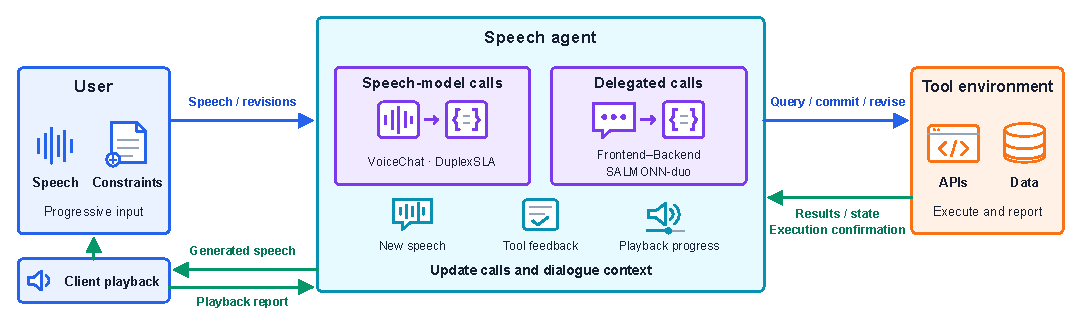
\includegraphics[width=\linewidth]{figures/tool_interaction_loop_en.pdf}
  \caption{The user--agent--environment loop in speech-tool interaction. Blue arrows carry requests and calls; green arrows carry execution feedback, speech delivered through client playback, and playback reports.}
  \label{fig:interaction-with-tools}
\end{figure}

\paragraph{Result integration and spoken feedback.}
Tool completion, integration into generation, and spoken delivery need not coincide. MoshiRAG retrieves between response onset and key content, injecting knowledge into ongoing generation~\citep{DBLP:journals/corr/abs-2604-12928}. GPT-Live distinguishes contextual updates from content to relay aloud; Gemini 3.8 Live's documented non-blocking configuration supports immediate, idle-time, or silent result handling~\citep{WEB:openai/live-delegation,WEB:google/live-capabilities}. Results may become obsolete before a speaking opportunity arises. $\tau$-Voice reports completion claims without corresponding calls~\citep{DBLP:journals/corr/abs-2603-13686}. Qwen-Audio-3.1-Realtime labels pre-call announcements as required, forbidden, or optional~\citep{DBLP:journals/corr/abs-2609-25176}. PACE repairs interrupted dialogue context using playback acknowledgments, avoiding reference to unplayed content~\citep{DBLP:journals/corr/abs-2608-07631}. Interpreting subsequent requests therefore depends on previously delivered information as well as execution state; playback records establish an opportunity to hear, not comprehension.

\paragraph{Call architectures and policy learning.}
Calls can be generated by the speech model or delegated to another decision module. VoiceChat generates structured calls through a separate function channel but excludes execution-time speech from response generation; DuplexSLA aligns speech and actions in shared 160-ms chunks~\citep{DBLP:journals/corr/abs-2609-21967,WEB:arxiv/2605.20755}. Delegated interfaces differ at runtime: Frontend--Backend suppresses frontend output during execution, whereas SALMONN-duo keeps it active and incorporates backend responses based on an invocation-time context snapshot~\citep{DBLP:journals/corr/abs-2609-19334,DBLP:journals/corr/abs-2609-34247}. Qwen3.5-Omni uses text-conditioned responses to supervise audio-conditioned generation~\citep{DBLP:journals/corr/abs-2604-15804}. VoxMind supplies reasoning and tool-use trajectories and retrieves tools on demand; SpeechGym combines call-level feedback with terminal rewards to train tool-use and spoken-response decisions, assuming instantaneous tool execution~\citep{DBLP:conf/acl/LiangCJCJLZPLZ26,DBLP:journals/corr/abs-2608-26432}.

\paragraph{Challenges.}
Speech-tool interaction must balance shorter waits with opportunities for revision. Complete arguments do not imply that the user has finished speaking, and earlier commitment may leave subsequent corrections too late to take effect. Early invocation, task updates, and stale-result filtering address different parts of this process, but revisable task records do not ensure revisable operations. Systems must determine both whether current evidence supports a call and what execution would commit them to, including what later speech could still change.

\paragraph{Outlook.}
Future action policies should adapt to incoming information and execution progress, jointly deciding when to keep listening, clarify, prepare, or commit. Where operations remain revisable, later speech should guide timely execution changes. Where effects have already occurred, systems should identify the limits of revision, explain consequences, and seek feasible remedies. Responsiveness should therefore be considered alongside effective user intervention, so that faster execution does not simply advance an intention that the user has already revised.

\begin{TakeawayBox}{Takeaways: Interaction with Tool Environment}
Speech-tool interaction couples unfolding requests with ongoing operations. Early calls can reduce waiting but may narrow the window for corrections. Returned results and played feedback inform subsequent confirmations and revisions. Systems must adapt actions to new information and execution progress, while distinguishing completed operations from those still changeable, enabling users to refine tasks as work proceeds.
\end{TakeawayBox}

\subsection{Interaction with Agents}
\label{sec:interaction-with-agents}

Full-duplex interaction allows speech to revise a task while an agent is speaking, delegating work, or returning results. Existing systems already use speech for inter-agent messaging, transcript repair, and specialist coordination~\citep{DBLP:journals/corr/abs-2401-03945,DBLP:journals/corr/abs-2601-10223,DBLP:journals/corr/abs-2606-07397}. The remaining issue is not communication alone, but whether responsibility, execution, and feedback stay aligned as the user's intent evolves.

\paragraph{Responsibility across frontend and backend.}
Multi-agent collaboration separates governance, participation, communication, and dialogue-history management~\citep{DBLP:journals/corr/abs-2502-14321,WEB:acl/2025.acl-long.1037}. Voice systems distribute these responsibilities across a responsive frontend, an orchestration layer, and asynchronous workers: Interaction Models and SALMONN-duo retain a conversational frontend, Gander mediates agentic execution through a runtime, and VoxMind and Qwen-Audio-Agent separate dialogue from delegated work~\citep{WEB:thinkingmachines/interaction-models,DBLP:journals/corr/abs-2609-34247,DBLP:journals/corr/abs-2609-08977,DBLP:conf/acl/LiangCJCJLZPLZ26,DBLP:journals/corr/abs-2609-25195}. These components respectively receive evidence, bind it to task state, and execute or verify bounded work.

\paragraph{Decision points within the delegation loop.}
Delegation introduces four decisions: when to launch work, whether later speech supplements or supersedes it, whether execution or only delivery should stop, and whether a returned result remains valid. Existing systems expose complementary controls: Gander reports lifecycle events, Qwen-Audio-Agent separates interruption from cancellation, AdaptDuplex identifies concurrent launches, and Jarvis associates typed decisions with versioned task records~\citep{DBLP:journals/corr/abs-2609-08977,DBLP:journals/corr/abs-2609-25195,DBLP:journals/corr/abs-2609-29217,WEB:arxiv/2610.23804}. A revision is reliable only when the control decision and the affected execution refer to the same task version.

\begin{figure*}[t]
  \centering
  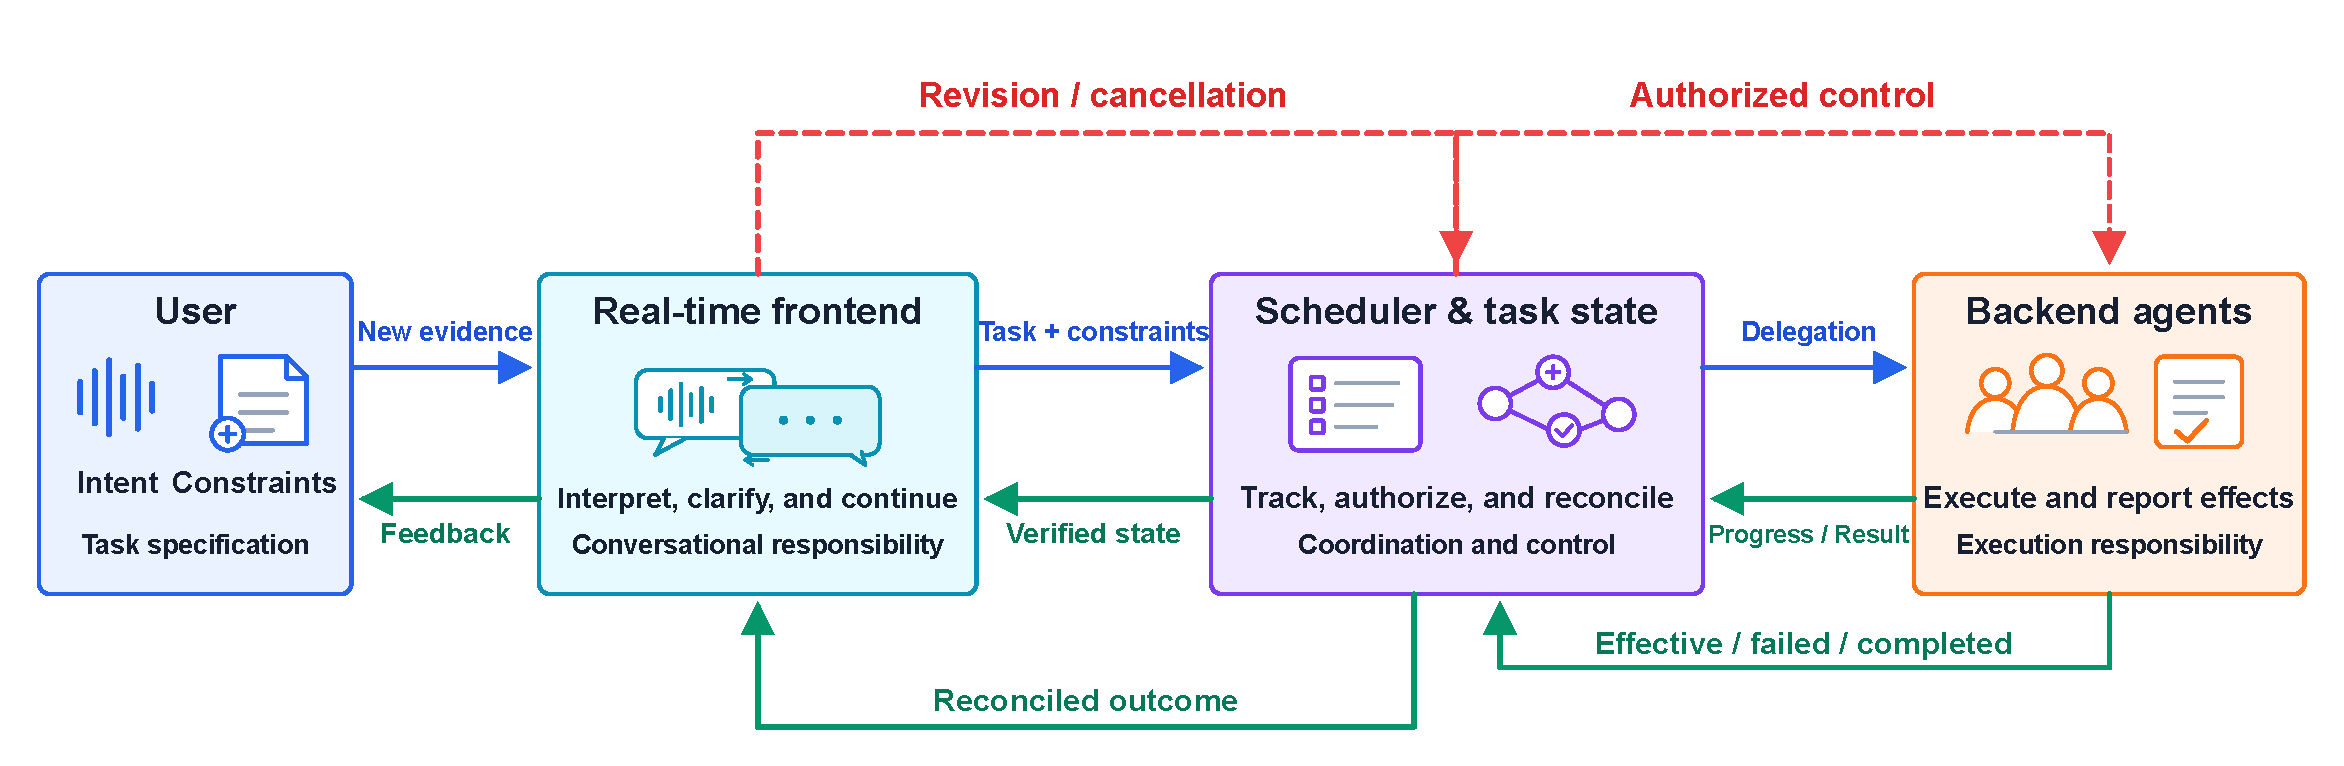
\includegraphics[width=\textwidth]{figures/agents-incremental-feedback.pdf}
  \caption{Information and control loops for a progressively specified task. The real-time frontend maintains the conversation, the scheduler binds new evidence to task state, and backend agents execute bounded work. Blue arrows carry task information, green arrows carry execution evidence, and red dashed arrows carry revision or cancellation.}
  \label{fig:agents-incremental-feedback}
\end{figure*}

\paragraph{Evaluation direction.}
Evaluation should follow revision scenarios rather than count agents or messages. Three measures are central: update latency until a state change is verified, update correctness for accepting the intended version and rejecting stale work, and feedback consistency between execution and what the user hears. Workflow frameworks provide observable state, durable execution, and cancellation primitives~\citep{WEB:google/adk-workflows,WEB:crewai/processes,WEB:microsoft/agent-framework,WEB:langchain/langgraph,WEB:a2a/specification}, while current benchmarks emphasize topology, long-horizon collaboration, protocol, memory, and routing~\citep{DBLP:conf/acl/ZhuDHYGWWQTJY25,DBLP:journals/corr/abs-2609-31590,WEB:arxiv/2610.04672}. Voice evaluation should additionally revise a constraint after delegation, replace a goal in flight, and cancel as a result arrives.

\paragraph{Challenges.}
The primary challenge is version-consistent accountability. Full duplex removes the turn boundary that normally fixes an interpretation before action, so different components may authorize, execute, and report different revisions. Shared context and successful message delivery are insufficient unless stale outcomes are rejected and the system can verify which change actually took effect.

\paragraph{Outlook.}
A promising direction is a speech-aware control layer connecting three accountability surfaces: a frontend that detects new evidence, a scheduler that owns task identity and revision authorization, and a backend that reports execution evidence. Future systems should combine explicit task versions, bounded cancellation, and delivery checks with benchmarks that trace each spoken revision from detection to verified execution and user-visible feedback.

\begin{TakeawayBox}{Takeaways: Interaction with Agents}
Agentic speech interaction requires more than multi-agent communication. Reliable delegation depends on explicit task identity, revision-aware control, stale-result rejection, and feedback grounded in the task version that actually executed.
\end{TakeawayBox}

\subsection{Interaction with Robotic Embodiment}
\label{sec:interaction-with-robotic-embodiment}
Speech enables users to specify and revise embodied tasks as execution changes the environment. Effective interaction links spoken intent to physical control and uses observed outcomes to guide subsequent planning and dialogue. Figure~\ref{fig:embodied-speech-overview} summarizes this revisable process.

\begin{figure}[!htbp]
  \centering
  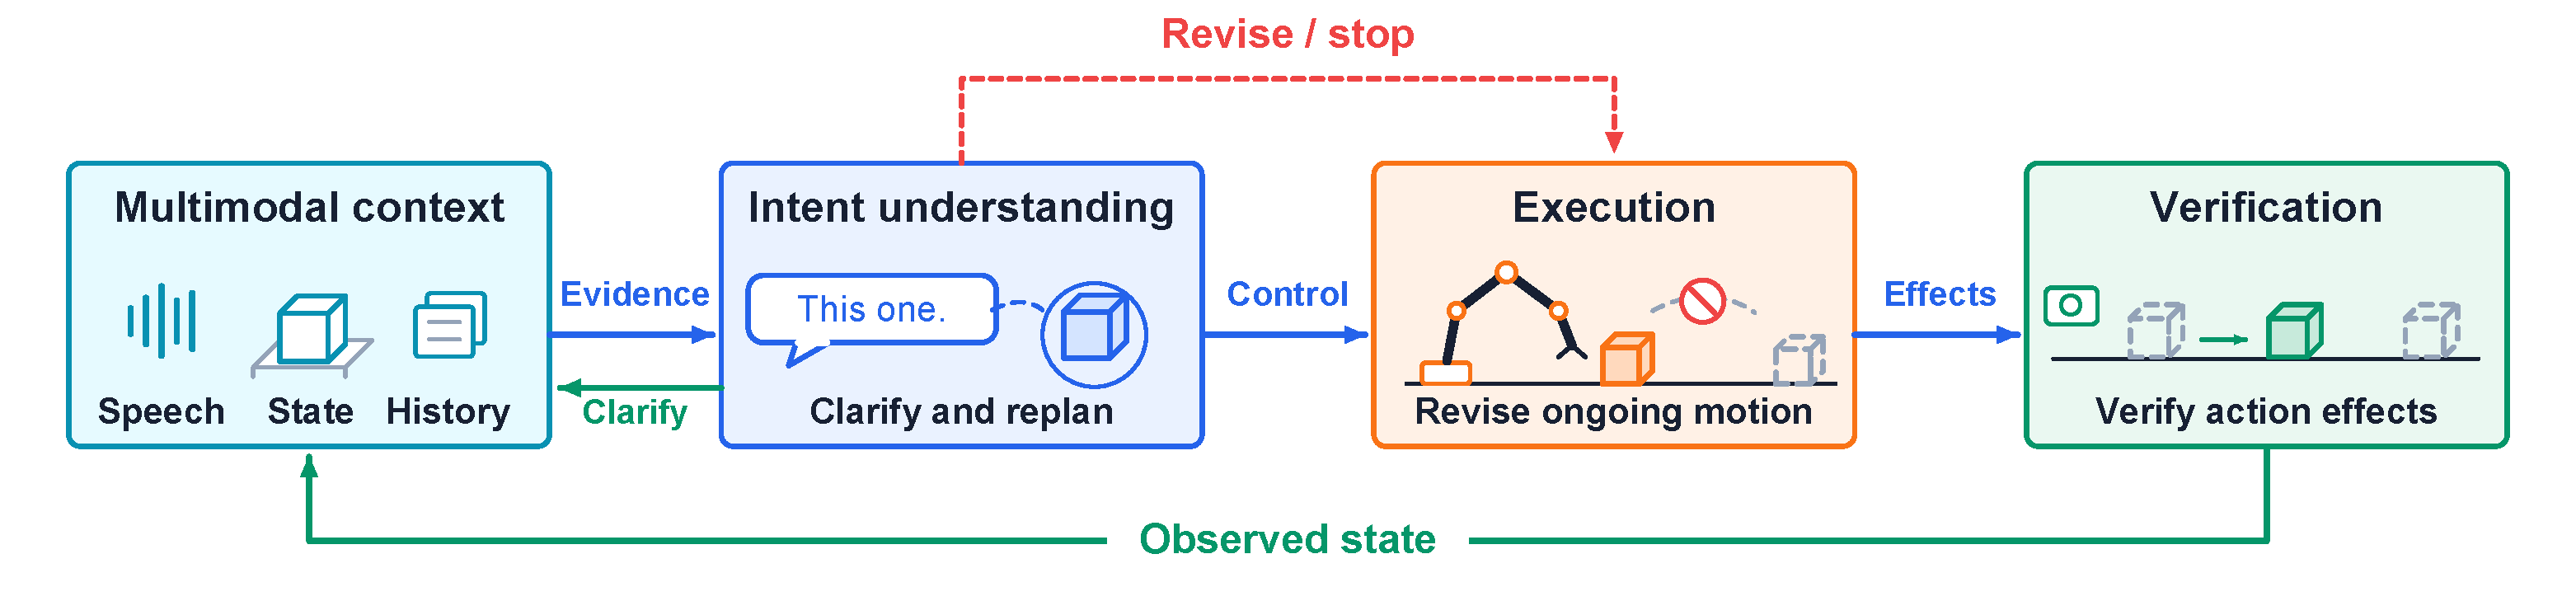
\includegraphics[width=\linewidth]{figures/embodied_speech_overview.pdf}
  \caption[Embodied speech interaction loop]{Embodied speech interaction as a revisable physical loop. Speech, current state, and interaction history inform intent understanding and planning. Blue arrows carry evidence, control, and action effects; the red dashed path denotes revision or stopping, and green arrows return clarification and observed state. Dashed object outlines represent prior or unexecuted positions. Full-duplex speech supports concurrent listening and speaking. Effective physical revision requires controller responses within temporal and safety limits, with subsequent planning and spoken feedback based on the state actually reached.}
  \label{fig:embodied-speech-overview}
\end{figure}

\paragraph{Intent Understanding and Clarification.}
Understanding spoken intent requires integrating speech with the current scene and task context. Visual context improves recognition of synthetically corrupted instructions~\citep{emb_chang2023}, while modular ASR--language--vision integration supports robot command generation~\citep{emb_nwankwo2024}. NMM-HRI combines pointing and RGB-D observations for reference resolution; VLAS conditions manipulation on speech and images and retrieves speaker-specific knowledge~\citep{emb_lai2025nmm,emb_zhao2025vlas}. When intent remains uncertain, dialogue can clarify the task before execution. RoboOmni infers intent from conversation, environmental sounds, and vision, then requests spoken confirmation before manipulation~\citep{emb_wang2025roboomni}. KnowNo complements these approaches by addressing when language-based robot planners should seek human assistance~\citep{emb_ren2023knowno}.

\paragraph{Revision, Replanning, and Feedback.}
Once execution begins, users can revise goals or constraints in response to observed behavior. Interactive Language accepts successive spoken instructions via ASR~\citep{emb_lynch2022interactive}; YAY Robot accepts a verbal stop followed by correction and incorporates interventions into subsequent policy learning~\citep{emb_shi2024yay}. Incremental language understanding coupled with online motion planning allows trajectories and constraints to change as an instruction unfolds~\citep{emb_abrams2025incremental}. Since revision does not erase prior physical effects, replanning must combine the updated instruction with the observed robot and scene state. HEAR preserves transient acoustic evidence across execution gaps for later control decisions~\citep{emb_nie2026hear}. Spoken feedback should convey observed progress, deviations, and uncertainty, giving users a basis for further correction or confirmation.

\paragraph{Full-Duplex Interaction.}
Full-duplex systems support intervention during robot speech through concurrent listening and speaking, incorporating incoming speech into the ongoing interaction. ELLSA coordinates modalities within a streaming model and evaluates action barge-in in simulation~\citep{emb_wang2026ellsa}; VITA-E uses parallel active and standby models for concurrent interaction, task switching, and stop requests on a physical humanoid~\citep{emb_liu2025vitae}. MIRA combines speech interruption handling with short, cancellable motion prefixes in companion interaction~\citep{emb_lin2026mira}. Deployment constraints remain relevant: the Pepper framework mutes its microphone during speech output because it lacks echo cancellation~\citep{emb_studerus2026pepper}. Beyond speech reception, physical responsiveness depends on how interventions reach and update the controller.

\paragraph{Challenges.}
Concurrent interaction must accommodate the different timescales of speech and physical execution. Recognition errors can redirect actions, while incomplete utterances, self-repairs, and overlapping speech make early interpretations provisional. Causal streaming restricts decisions to available evidence; buffering and committed motion can delay correction until physical effects are irreversible. VAP addresses conversational turn prediction, and RASSG studies repair-aware cancellation under simulated tool execution~\citep{emb_inoue2024vap,emb_hu2026rassg}. Applying these mechanisms to robots requires validation across speech reception, controller updates, physical stopping, and task outcomes. Evaluation must also establish whether replanning and spoken reports remain consistent with the resulting state.

\paragraph{Outlook.}
In future long-horizon assistance and collaborative manipulation, speech could serve as an incremental task specification. Users could start with an approximate goal and refine preferences, references, and constraints while observing execution. By integrating these updates with interaction history and current observations, robots could maintain a revisable interpretation of intent, adapt their plans, and seek clarification before committing to uncertain actions. Spoken output would make this process accessible by distinguishing completed steps, current progress, unresolved uncertainty, and intended next actions. Such exchanges could support the continuous joint refinement of tasks, bringing robot behavior into closer alignment with users' evolving goals.

\begin{TakeawayBox}{Takeaways: Interaction with Robotic Embodiment}
Speech supports incremental task refinement; full-duplex interaction permits intervention during system speech. Effective revision requires control updates within task-specific temporal and safety limits, followed by replanning from observed physical outcomes. Accurate spoken feedback enables further correction and confirmation, sustaining alignment with evolving user goals.
\end{TakeawayBox}




\subsection{Interaction with Self-Memory and Lifelong Context}
\label{sec:interaction-with-memory}

Memory enables spoken dialogue systems to maintain information beyond the current utterance and reuse it across later interactions. In full-duplex dialogue, however, interpretations may change as speech unfolds, making it necessary to distinguish provisional evidence from confirmed information and preserve the validity of subsequent revisions. Effective memory interaction therefore concerns not only what is retained, but when information becomes valid and whether superseded information continues to influence later decisions. Figure~\ref{fig:memory-overview} illustrates this process.

\begin{figure}[!htbp]
\centering
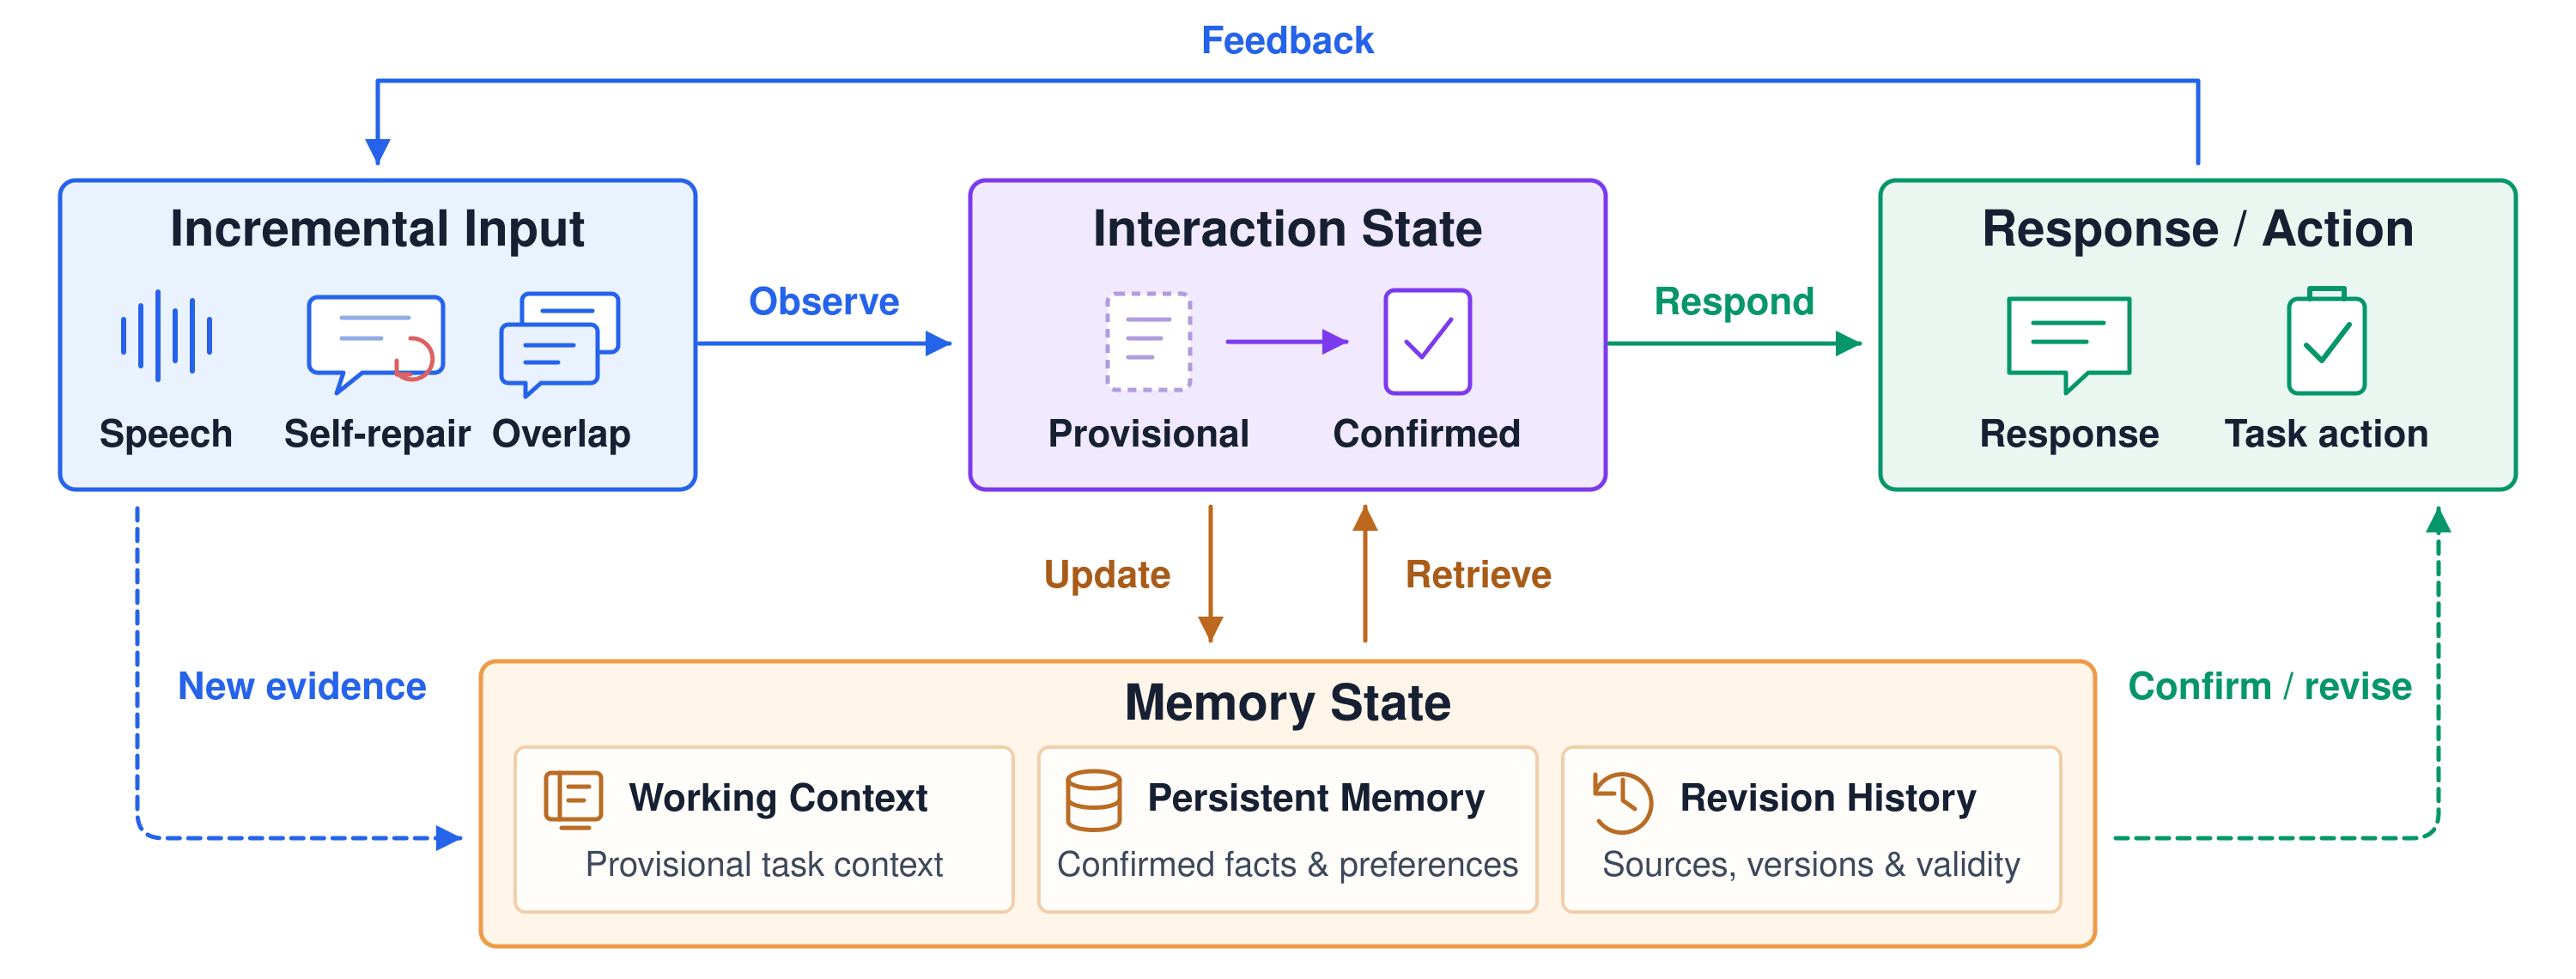
\includegraphics[width=\linewidth]{figures/memory_overview.png}
\caption{Memory-supported interaction in full-duplex spoken dialogue. Incremental speech and interaction context inform memory formation, retrieval, revision, and persistence. Corrections and deletions may change the validity of stored information and its use in subsequent interactions.}
\label{fig:memory-overview}
\end{figure}

\paragraph{Memory Formation and Attribution.}
Forming persistent memory requires selecting information from ongoing interaction and preserving its source and conversational context. EgoMem processes audiovisual streams through asynchronous retrieval, dialogue, and memory management, using detected interaction boundaries to extract and update user information~\citep{DBLP:journals/corr/abs-2509-11914}. In multi-party settings, attribution becomes more complex. VoiceTrace supports speaker-conditioned speech retrieval~\citep{DBLP:journals/corr/abs-2609-18521}, while SpeakerMem-R1 organizes speaker-labeled messages and derived personal and group states~\citep{DBLP:journals/corr/abs-2609-26780}. VoxPolyMem further represents participant relationships and interaction history to support memory retrieval across multi-party spoken sessions~\citep{DBLP:journals/corr/abs-2609-32522}. Beyond lexical content, VoiceMem distinguishes context-dependent affective evidence from more persistent user characteristics~\citep{DBLP:journals/corr/abs-2608-26005}. These approaches improve memory construction and attribution, but identifying the speaker or extracting a fact does not establish whether an incomplete, inferred, or corrected statement should become persistent memory. In full-duplex interaction, such commitment must account for subsequent clarification and self-repair.

\paragraph{Temporal Revision and Memory Updating.}
Persistent information may change across turns and sessions, requiring memory systems to distinguish current facts from their historical versions. Zep represents evolving information through a temporal knowledge graph, preserving source-linked episodes and the validity of relationships~\citep{DBLP:journals/corr/abs-2501-13956}. BELIEFMEM treats conversational updates as belief revisions, maintaining predecessor relationships between superseded and current beliefs~\citep{meng-etal-2026-beliefmem}. APEX-MEM retains temporal history in an append-only property graph and resolves conflicting information during retrieval~\citep{DBLP:conf/acl/BanerjeeMSMC26}, while TSHMem incorporates temporal constraints into graph-based evidence selection to reduce retrieval of outdated information~\citep{xu-etal-2026-tshmem}. For spoken interaction, VoiceMem performs asynchronous memory reconciliation through add, update, delete, and keep operations~\citep{DBLP:journals/corr/abs-2608-26005}. Voice Memory for Agentic Speech Recognition similarly uses an editable memory file and score-gated updates to constrain recognition correction without parameter changes~\citep{DBLP:journals/corr/abs-2607-26410}. These mechanisms address different parts of memory revision. However, updating a stored record or selecting the correct version at retrieval does not necessarily invalidate information already incorporated into summaries, user profiles, cached context, or ongoing tasks.

\paragraph{Persistent Memory and Evaluation.}
Reliable memory revision must remain effective beyond the turn in which a correction occurs. LongMemEval evaluates knowledge updates and temporal reasoning across extended conversational histories~\citep{DBLP:conf/iclr/WuWYZCY25}, while ChronoScope examines whether temporal scope is preserved or revised across successive dialogue turns~\citep{DBLP:conf/acl/AtriJH26}. For spoken interaction, VoxMem evaluates multi-session memory involving speech content, speaker identity, paralinguistic information, and temporal tracking~\citep{DBLP:journals/corr/abs-2609-32607}. ContextDialog examines conversational context recall and utilization in voice interaction models~\citep{contextdialog}. Beyond answer correctness, MemEval diagnoses failures across memory extraction, updating, retrieval, and utilization~\citep{wang-etal-2026-memories}, and UTILMEM examines whether retrieved evidence is integrated reliably into downstream responses~\citep{qing-etal-2026-utilmem}. Together, these evaluations expose limitations in temporal reasoning, attribution, and memory utilization. Yet correctly answering a question about a revised fact does not by itself establish that obsolete information has been invalidated throughout persistent storage or excluded from subsequent task decisions.

\paragraph{Challenges.}
Memory revision in full-duplex dialogue faces both temporal and state-consistency constraints. Incomplete utterances, overlapping speech, and self-repairs make it difficult to determine when information should be committed, while speaker identification alone cannot establish addressee, conversational function, or authority to modify a record. Once committed, corrections must propagate beyond the original memory entry. Forgetting Without Restarting demonstrates that deleting explicit memory can leave revoked information influential through derived execution state, and investigates provenance-guided replay to address this problem~\citep{DBLP:journals/corr/abs-2609-04875}. Comparable consistency requirements arise across summaries, retrieval indexes, speaker profiles, and pending task operations. Deletion must also be distinguished from historical invalidation, and task cancellation from factual correction. Current evaluations rarely inspect these states together under continuous speech. Establishing reliable revision therefore requires measuring when an update takes effect, which representations remain affected, and whether outdated evidence still changes subsequent behavior.

\paragraph{Outlook.}
Future spoken agents could maintain versioned, source-aware memory in which provisional interpretations, confirmed facts, historical records, and deleted information have explicitly distinguished roles. Incremental speech processing would support early retrieval and response preparation without prematurely committing uncertain evidence. Corrections could then update the active memory state, preserve appropriate historical relationships, and trigger revalidation of dependent summaries, retrievals, and tasks. For multi-party interaction, such mechanisms would additionally track speaker attribution, participation, and conversational authority. Evaluation should follow a revision from its initial utterance through confirmation, storage, retrieval, and subsequent decisions, including across sessions. This would shift lifelong memory assessment from recalling prior conversations toward verifying that evolving information remains consistent with the system's ongoing behavior.

\begin{TakeawayBox}{Takeaways: Self-Memory and Lifelong Context}
Memory-level revisability requires distinguishing provisional speech interpretations from committed information, preserving source and temporal validity, and preventing superseded records from influencing current decisions. Existing work advances memory attribution, temporal updating, and cross-session evaluation, but reliable propagation across stored representations and ongoing task state remains insufficiently established.
\end{TakeawayBox}



\section{Agentic Audio Interaction}
\label{sec:agentic-audio-interaction}

% TODO: Introduce spoken interaction with tools, agents, embodied systems, and memory.
Full-duplex speech interaction is usually evaluated by whether a system can listen and speak concurrently, manage turn transitions, and respond to interruptions. Once speech models are connected to tools, delegated agents, embodied systems, and persistent memory, however, later speech may need to change more than the current response: it may revise a tool call, transfer task responsibility, redirect a physical action, or invalidate information used in future decisions. We use \textbf{speech-grounded task revisability} to denote the ability to interpret incremental speech as evidence for maintaining, modifying, suspending, or revoking task state, and to propagate that decision consistently through execution, feedback, and memory. TOOL, AGENT, EMB, and MEM identify four scopes of this problem: revising an external operation, assigning control over the revision, changing a physical action, and preserving the revised information over time.

\subsection{Interaction with Tool Environment}
\label{sec:interaction-with-tool-environment}
% TODO: Cover speech-driven tool use and tool orchestration.
Tool interaction forms an information loop between users, agents, and environments. Spoken arguments and constraints emerge incrementally; later corrections may conflict with ongoing operations. Feedback is also delivered progressively, informing subsequent confirmations and revisions. Systems must therefore let new information affect relevant operations and interpret subsequent requests against actual execution and played content.

\paragraph{Intent interpretation and call preparation.}
Forming calls requires distinguishing misrecognized arguments from incomplete requests. Synthetic user-style queries adapt tool embeddings to improve noisy-transcript retrieval~\citep{WEB:isca/zorila26_interspeech}, while Spoken Function Calling conditions output on function schemas and environmental context, marking missing arguments as \texttt{NAN}~\citep{DBLP:journals/corr/abs-2608-05126}. BFCL Audio, Full-Duplex-Bench-v3, and VGBench examine acoustic corruption, disfluency and self-correction, and whether speech addresses the agent, respectively~\citep{WEB:pmlr/v306/mao26b,DBLP:journals/corr/abs-2604-04847,DBLP:journals/corr/abs-2609-32536}. Stream RAG retrieves from speech prefixes, overlapping retrieval with listening~\citep{DBLP:journals/corr/abs-2510-02044}. Heard Enough to Act learns early invocation from supervision marking sufficient tool and argument evidence, but remains limited by false triggers~\citep{WEB:arxiv/2610.34653}. These studies address incomplete or unreliable input, without establishing that the request has stabilized.

\paragraph{Request revision during execution.}
Later speech must be associated with an existing task to affect execution. In simulated streaming-transcript interaction, SIA revises speculative calls through identifiers and dependencies, discarding obsolete returns that have not yet entered context~\citep{DBLP:journals/corr/abs-2605-13360}. Gander routes updates to the active task and, where the backend supports them, handles side questions through read-only forks that preserve the main task's execution context~\citep{DBLP:journals/corr/abs-2609-08977}. StepAudio 3 Realtime distinguishes task updates from unrelated speech; Qwen-Audio-Agent separates task cancellation from speech interruption~\citep{WEB:arxiv/2609.14005,DBLP:journals/corr/abs-2609-25195}. DuplexAgent-RSI records task versions and delivery histories: late returns remain recorded but cannot restore cancelled or superseded work to delivery eligibility~\citep{WEB:arxiv/2610.11299}. This separates execution evidence from permission to deliver results.

\begin{figure}[t]
  \centering
  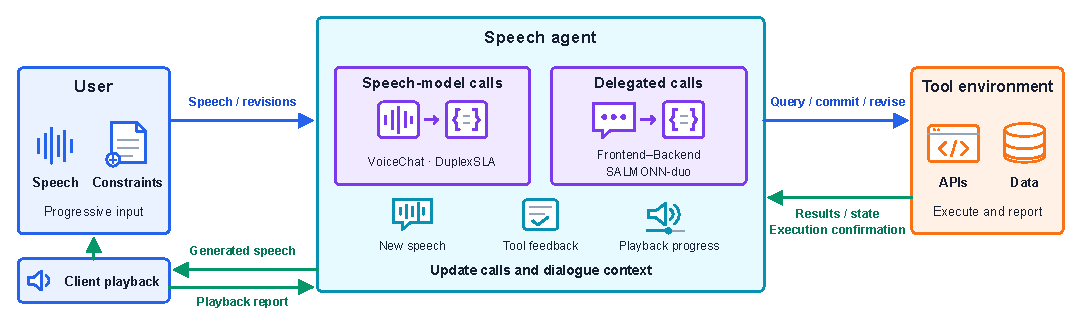
\includegraphics[width=\linewidth]{figures/tool_interaction_loop_en.pdf}
  \caption{The user--agent--environment loop in speech-tool interaction. Blue arrows carry requests and calls; green arrows carry execution feedback, speech delivered through client playback, and playback reports.}
  \label{fig:interaction-with-tools}
\end{figure}

\paragraph{Result integration and spoken feedback.}
Tool completion, integration into generation, and spoken delivery need not coincide. MoshiRAG retrieves between response onset and key content, injecting knowledge into ongoing generation~\citep{DBLP:journals/corr/abs-2604-12928}. GPT-Live distinguishes contextual updates from content to relay aloud; Gemini 3.8 Live's documented non-blocking configuration supports immediate, idle-time, or silent result handling~\citep{WEB:openai/live-delegation,WEB:google/live-capabilities}. Results may become obsolete before a speaking opportunity arises. $\tau$-Voice reports completion claims without corresponding calls~\citep{DBLP:journals/corr/abs-2603-13686}. Qwen-Audio-3.1-Realtime labels pre-call announcements as required, forbidden, or optional~\citep{DBLP:journals/corr/abs-2609-25176}. PACE repairs interrupted dialogue context using playback acknowledgments, avoiding reference to unplayed content~\citep{DBLP:journals/corr/abs-2608-07631}. Interpreting subsequent requests therefore depends on previously delivered information as well as execution state; playback records establish an opportunity to hear, not comprehension.

\paragraph{Call architectures and policy learning.}
Calls can be generated by the speech model or delegated to another decision module. VoiceChat generates structured calls through a separate function channel but excludes execution-time speech from response generation; DuplexSLA aligns speech and actions in shared 160-ms chunks~\citep{DBLP:journals/corr/abs-2609-21967,WEB:arxiv/2605.20755}. Delegated interfaces differ at runtime: Frontend--Backend suppresses frontend output during execution, whereas SALMONN-duo keeps it active and incorporates backend responses based on an invocation-time context snapshot~\citep{DBLP:journals/corr/abs-2609-19334,DBLP:journals/corr/abs-2609-34247}. Qwen3.5-Omni uses text-conditioned responses to supervise audio-conditioned generation~\citep{DBLP:journals/corr/abs-2604-15804}. VoxMind supplies reasoning and tool-use trajectories and retrieves tools on demand; SpeechGym combines call-level feedback with terminal rewards to train tool-use and spoken-response decisions, assuming instantaneous tool execution~\citep{DBLP:conf/acl/LiangCJCJLZPLZ26,DBLP:journals/corr/abs-2608-26432}.

\paragraph{Challenges.}
Speech-tool interaction must balance shorter waits with opportunities for revision. Complete arguments do not imply that the user has finished speaking, and earlier commitment may leave subsequent corrections too late to take effect. Early invocation, task updates, and stale-result filtering address different parts of this process, but revisable task records do not ensure revisable operations. Systems must determine both whether current evidence supports a call and what execution would commit them to, including what later speech could still change.

\paragraph{Outlook.}
Future action policies should adapt to incoming information and execution progress, jointly deciding when to keep listening, clarify, prepare, or commit. Where operations remain revisable, later speech should guide timely execution changes. Where effects have already occurred, systems should identify the limits of revision, explain consequences, and seek feasible remedies. Responsiveness should therefore be considered alongside effective user intervention, so that faster execution does not simply advance an intention that the user has already revised.

\begin{TakeawayBox}{Takeaways: Interaction with Tool Environment}
Speech-tool interaction couples unfolding requests with ongoing operations. Early calls can reduce waiting but may narrow the window for corrections. Returned results and played feedback inform subsequent confirmations and revisions. Systems must adapt actions to new information and execution progress, while distinguishing completed operations from those still changeable, enabling users to refine tasks as work proceeds.
\end{TakeawayBox}

\subsection{Interaction with Agents}
\label{sec:interaction-with-agents}

Full-duplex interaction allows speech to revise a task while an agent is speaking, delegating work, or returning results. Existing systems already use speech for inter-agent messaging, transcript repair, and specialist coordination~\citep{DBLP:journals/corr/abs-2401-03945,DBLP:journals/corr/abs-2601-10223,DBLP:journals/corr/abs-2606-07397}. The remaining issue is not communication alone, but whether responsibility, execution, and feedback stay aligned as the user's intent evolves.

\paragraph{Responsibility across frontend and backend.}
Multi-agent collaboration separates governance, participation, communication, and dialogue-history management~\citep{DBLP:journals/corr/abs-2502-14321,WEB:acl/2025.acl-long.1037}. Voice systems distribute these responsibilities across a responsive frontend, an orchestration layer, and asynchronous workers: Interaction Models and SALMONN-duo retain a conversational frontend, Gander mediates agentic execution through a runtime, and VoxMind and Qwen-Audio-Agent separate dialogue from delegated work~\citep{WEB:thinkingmachines/interaction-models,DBLP:journals/corr/abs-2609-34247,DBLP:journals/corr/abs-2609-08977,DBLP:conf/acl/LiangCJCJLZPLZ26,DBLP:journals/corr/abs-2609-25195}. These components respectively receive evidence, bind it to task state, and execute or verify bounded work.

\paragraph{Decision points within the delegation loop.}
Delegation introduces four decisions: when to launch work, whether later speech supplements or supersedes it, whether execution or only delivery should stop, and whether a returned result remains valid. Existing systems expose complementary controls: Gander reports lifecycle events, Qwen-Audio-Agent separates interruption from cancellation, AdaptDuplex identifies concurrent launches, and Jarvis associates typed decisions with versioned task records~\citep{DBLP:journals/corr/abs-2609-08977,DBLP:journals/corr/abs-2609-25195,DBLP:journals/corr/abs-2609-29217,WEB:arxiv/2610.23804}. A revision is reliable only when the control decision and the affected execution refer to the same task version.

\begin{figure*}[t]
  \centering
  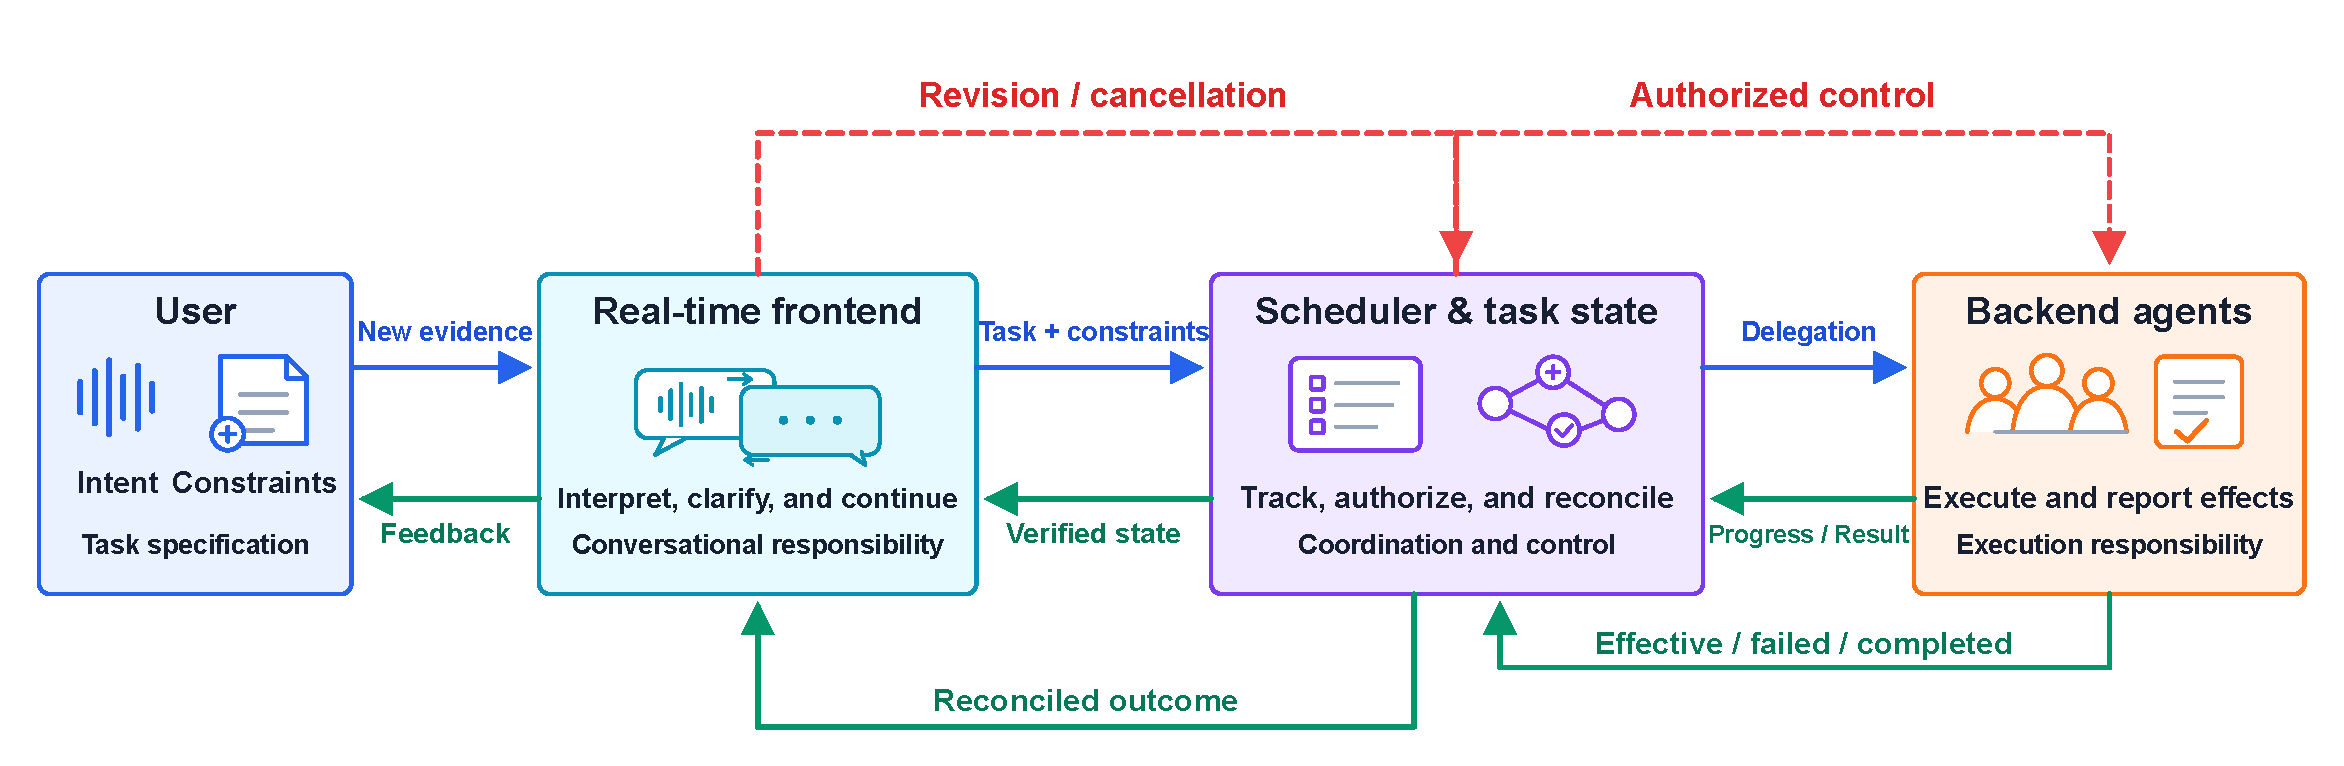
\includegraphics[width=\textwidth]{figures/agents-incremental-feedback.pdf}
  \caption{Information and control loops for a progressively specified task. The real-time frontend maintains the conversation, the scheduler binds new evidence to task state, and backend agents execute bounded work. Blue arrows carry task information, green arrows carry execution evidence, and red dashed arrows carry revision or cancellation.}
  \label{fig:agents-incremental-feedback}
\end{figure*}

\paragraph{Evaluation direction.}
Evaluation should follow revision scenarios rather than count agents or messages. Three measures are central: update latency until a state change is verified, update correctness for accepting the intended version and rejecting stale work, and feedback consistency between execution and what the user hears. Workflow frameworks provide observable state, durable execution, and cancellation primitives~\citep{WEB:google/adk-workflows,WEB:crewai/processes,WEB:microsoft/agent-framework,WEB:langchain/langgraph,WEB:a2a/specification}, while current benchmarks emphasize topology, long-horizon collaboration, protocol, memory, and routing~\citep{DBLP:conf/acl/ZhuDHYGWWQTJY25,DBLP:journals/corr/abs-2609-31590,WEB:arxiv/2610.04672}. Voice evaluation should additionally revise a constraint after delegation, replace a goal in flight, and cancel as a result arrives.

\paragraph{Challenges.}
The primary challenge is version-consistent accountability. Full duplex removes the turn boundary that normally fixes an interpretation before action, so different components may authorize, execute, and report different revisions. Shared context and successful message delivery are insufficient unless stale outcomes are rejected and the system can verify which change actually took effect.

\paragraph{Outlook.}
A promising direction is a speech-aware control layer connecting three accountability surfaces: a frontend that detects new evidence, a scheduler that owns task identity and revision authorization, and a backend that reports execution evidence. Future systems should combine explicit task versions, bounded cancellation, and delivery checks with benchmarks that trace each spoken revision from detection to verified execution and user-visible feedback.

\begin{TakeawayBox}{Takeaways: Interaction with Agents}
Agentic speech interaction requires more than multi-agent communication. Reliable delegation depends on explicit task identity, revision-aware control, stale-result rejection, and feedback grounded in the task version that actually executed.
\end{TakeawayBox}

\subsection{Interaction with Robotic Embodiment}
\label{sec:interaction-with-robotic-embodiment}
Speech enables users to specify and revise embodied tasks as execution changes the environment. Effective interaction links spoken intent to physical control and uses observed outcomes to guide subsequent planning and dialogue. Figure~\ref{fig:embodied-speech-overview} summarizes this revisable process.

\begin{figure}[!htbp]
  \centering
  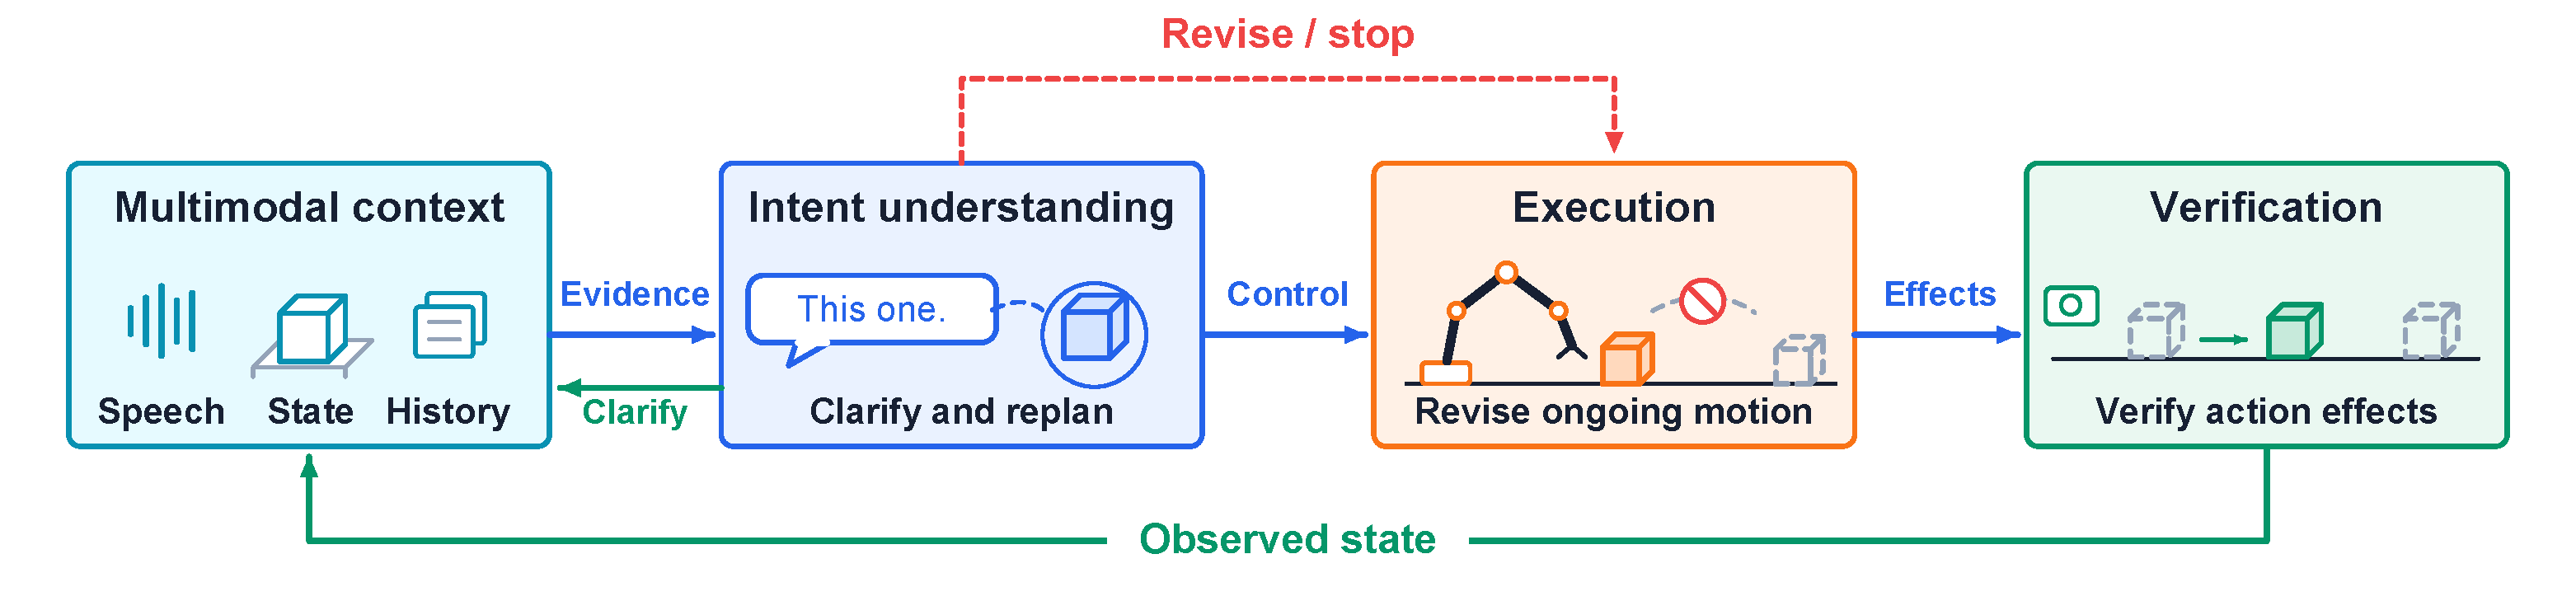
\includegraphics[width=\linewidth]{figures/embodied_speech_overview.pdf}
  \caption[Embodied speech interaction loop]{Embodied speech interaction as a revisable physical loop. Speech, current state, and interaction history inform intent understanding and planning. Blue arrows carry evidence, control, and action effects; the red dashed path denotes revision or stopping, and green arrows return clarification and observed state. Dashed object outlines represent prior or unexecuted positions. Full-duplex speech supports concurrent listening and speaking. Effective physical revision requires controller responses within temporal and safety limits, with subsequent planning and spoken feedback based on the state actually reached.}
  \label{fig:embodied-speech-overview}
\end{figure}

\paragraph{Intent Understanding and Clarification.}
Understanding spoken intent requires integrating speech with the current scene and task context. Visual context improves recognition of synthetically corrupted instructions~\citep{emb_chang2023}, while modular ASR--language--vision integration supports robot command generation~\citep{emb_nwankwo2024}. NMM-HRI combines pointing and RGB-D observations for reference resolution; VLAS conditions manipulation on speech and images and retrieves speaker-specific knowledge~\citep{emb_lai2025nmm,emb_zhao2025vlas}. When intent remains uncertain, dialogue can clarify the task before execution. RoboOmni infers intent from conversation, environmental sounds, and vision, then requests spoken confirmation before manipulation~\citep{emb_wang2025roboomni}. KnowNo complements these approaches by addressing when language-based robot planners should seek human assistance~\citep{emb_ren2023knowno}.

\paragraph{Revision, Replanning, and Feedback.}
Once execution begins, users can revise goals or constraints in response to observed behavior. Interactive Language accepts successive spoken instructions via ASR~\citep{emb_lynch2022interactive}; YAY Robot accepts a verbal stop followed by correction and incorporates interventions into subsequent policy learning~\citep{emb_shi2024yay}. Incremental language understanding coupled with online motion planning allows trajectories and constraints to change as an instruction unfolds~\citep{emb_abrams2025incremental}. Since revision does not erase prior physical effects, replanning must combine the updated instruction with the observed robot and scene state. HEAR preserves transient acoustic evidence across execution gaps for later control decisions~\citep{emb_nie2026hear}. Spoken feedback should convey observed progress, deviations, and uncertainty, giving users a basis for further correction or confirmation.

\paragraph{Full-Duplex Interaction.}
Full-duplex systems support intervention during robot speech through concurrent listening and speaking, incorporating incoming speech into the ongoing interaction. ELLSA coordinates modalities within a streaming model and evaluates action barge-in in simulation~\citep{emb_wang2026ellsa}; VITA-E uses parallel active and standby models for concurrent interaction, task switching, and stop requests on a physical humanoid~\citep{emb_liu2025vitae}. MIRA combines speech interruption handling with short, cancellable motion prefixes in companion interaction~\citep{emb_lin2026mira}. Deployment constraints remain relevant: the Pepper framework mutes its microphone during speech output because it lacks echo cancellation~\citep{emb_studerus2026pepper}. Beyond speech reception, physical responsiveness depends on how interventions reach and update the controller.

\paragraph{Challenges.}
Concurrent interaction must accommodate the different timescales of speech and physical execution. Recognition errors can redirect actions, while incomplete utterances, self-repairs, and overlapping speech make early interpretations provisional. Causal streaming restricts decisions to available evidence; buffering and committed motion can delay correction until physical effects are irreversible. VAP addresses conversational turn prediction, and RASSG studies repair-aware cancellation under simulated tool execution~\citep{emb_inoue2024vap,emb_hu2026rassg}. Applying these mechanisms to robots requires validation across speech reception, controller updates, physical stopping, and task outcomes. Evaluation must also establish whether replanning and spoken reports remain consistent with the resulting state.

\paragraph{Outlook.}
In future long-horizon assistance and collaborative manipulation, speech could serve as an incremental task specification. Users could start with an approximate goal and refine preferences, references, and constraints while observing execution. By integrating these updates with interaction history and current observations, robots could maintain a revisable interpretation of intent, adapt their plans, and seek clarification before committing to uncertain actions. Spoken output would make this process accessible by distinguishing completed steps, current progress, unresolved uncertainty, and intended next actions. Such exchanges could support the continuous joint refinement of tasks, bringing robot behavior into closer alignment with users' evolving goals.

\begin{TakeawayBox}{Takeaways: Interaction with Robotic Embodiment}
Speech supports incremental task refinement; full-duplex interaction permits intervention during system speech. Effective revision requires control updates within task-specific temporal and safety limits, followed by replanning from observed physical outcomes. Accurate spoken feedback enables further correction and confirmation, sustaining alignment with evolving user goals.
\end{TakeawayBox}




\subsection{Interaction with Self-Memory and Lifelong Context}
\label{sec:interaction-with-memory}

Memory enables spoken dialogue systems to maintain information beyond the current utterance and reuse it across later interactions. In full-duplex dialogue, however, interpretations may change as speech unfolds, making it necessary to distinguish provisional evidence from confirmed information and preserve the validity of subsequent revisions. Effective memory interaction therefore concerns not only what is retained, but when information becomes valid and whether superseded information continues to influence later decisions. Figure~\ref{fig:memory-overview} illustrates this process.

\begin{figure}[!htbp]
\centering
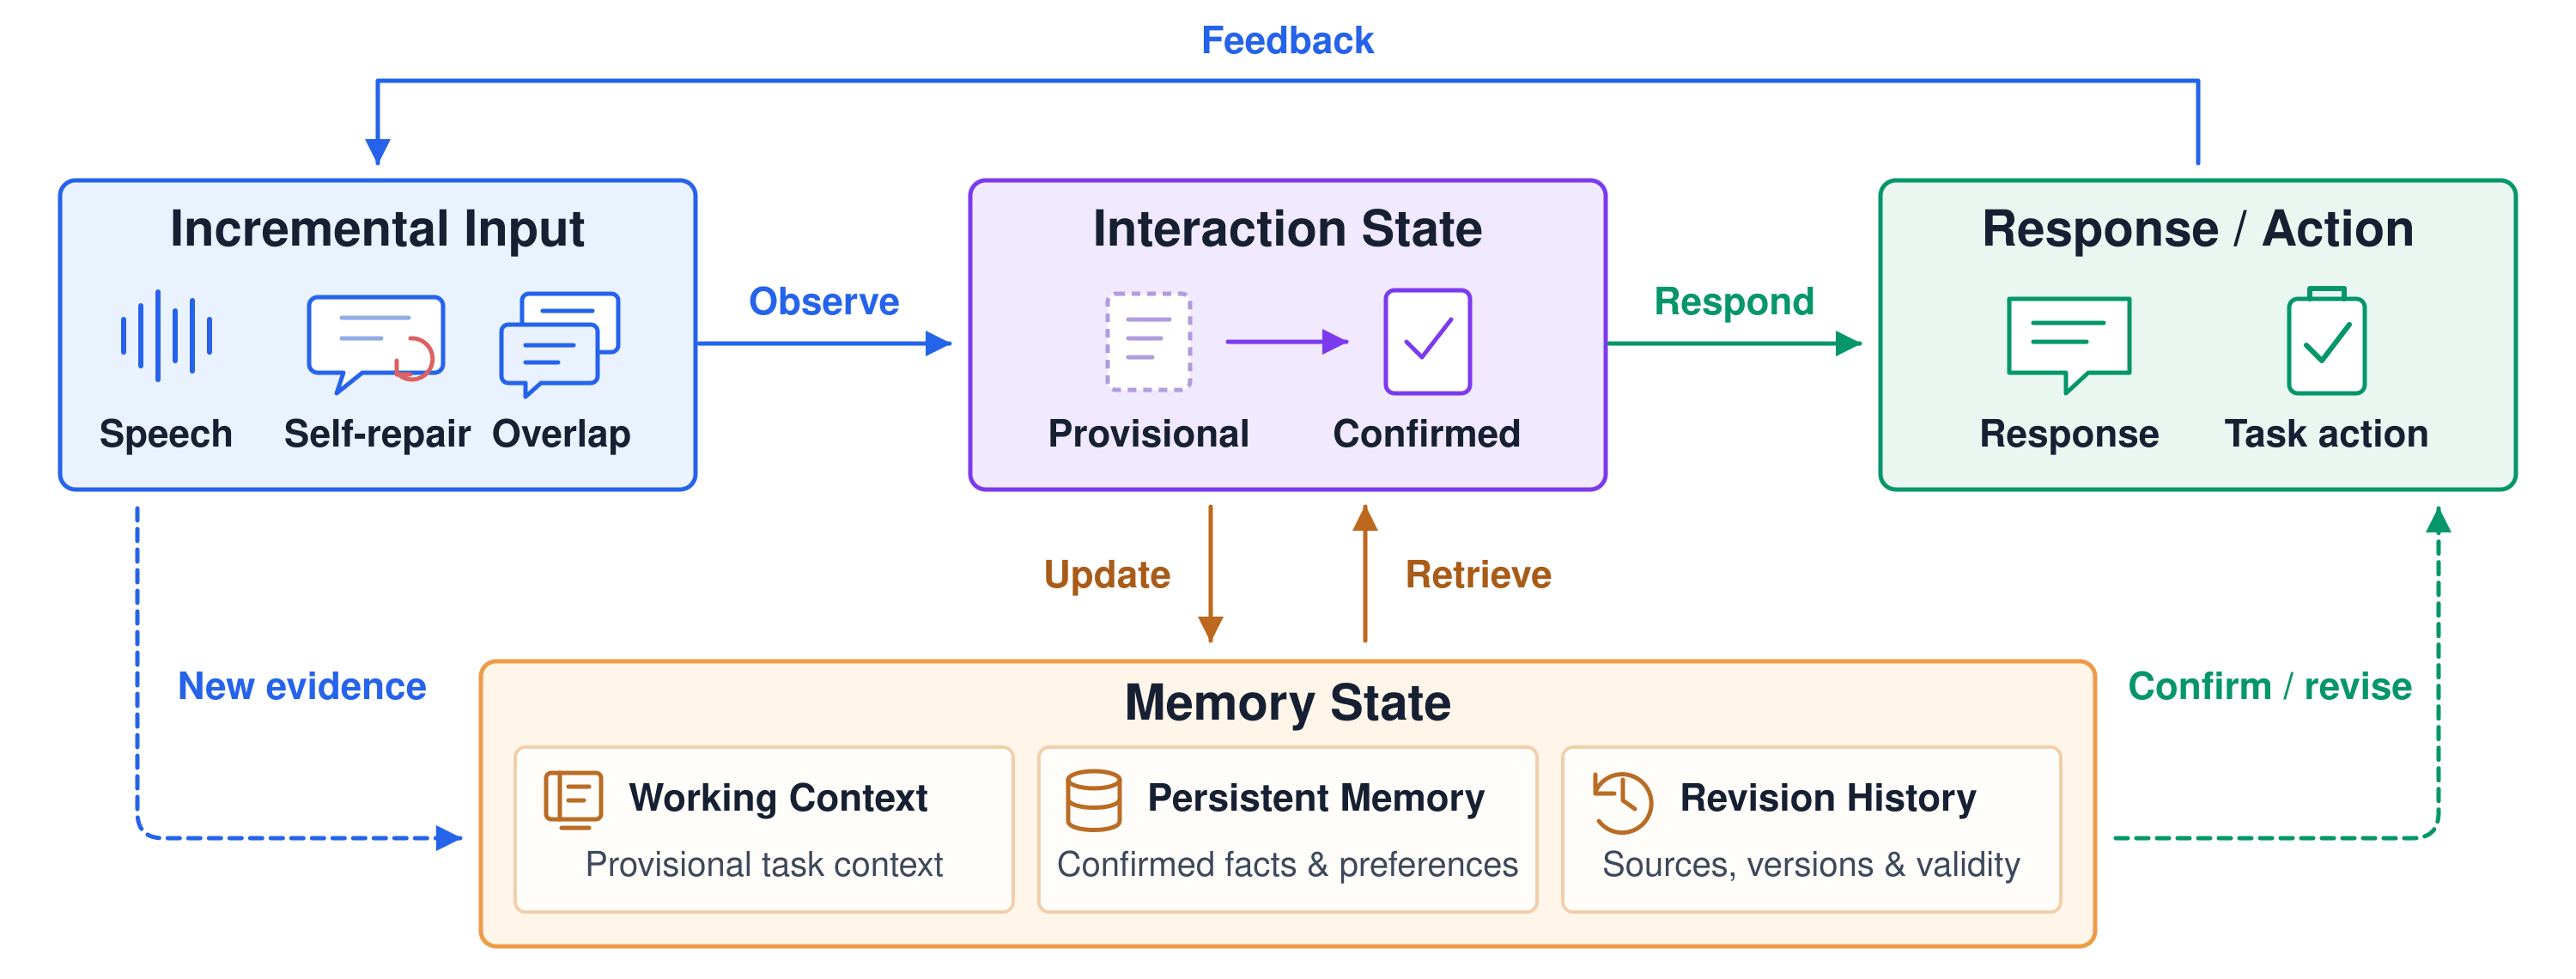
\includegraphics[width=\linewidth]{figures/memory_overview.png}
\caption{Memory-supported interaction in full-duplex spoken dialogue. Incremental speech and interaction context inform memory formation, retrieval, revision, and persistence. Corrections and deletions may change the validity of stored information and its use in subsequent interactions.}
\label{fig:memory-overview}
\end{figure}

\paragraph{Memory Formation and Attribution.}
Forming persistent memory requires selecting information from ongoing interaction and preserving its source and conversational context. EgoMem processes audiovisual streams through asynchronous retrieval, dialogue, and memory management, using detected interaction boundaries to extract and update user information~\citep{DBLP:journals/corr/abs-2509-11914}. In multi-party settings, attribution becomes more complex. VoiceTrace supports speaker-conditioned speech retrieval~\citep{DBLP:journals/corr/abs-2609-18521}, while SpeakerMem-R1 organizes speaker-labeled messages and derived personal and group states~\citep{DBLP:journals/corr/abs-2609-26780}. VoxPolyMem further represents participant relationships and interaction history to support memory retrieval across multi-party spoken sessions~\citep{DBLP:journals/corr/abs-2609-32522}. Beyond lexical content, VoiceMem distinguishes context-dependent affective evidence from more persistent user characteristics~\citep{DBLP:journals/corr/abs-2608-26005}. These approaches improve memory construction and attribution, but identifying the speaker or extracting a fact does not establish whether an incomplete, inferred, or corrected statement should become persistent memory. In full-duplex interaction, such commitment must account for subsequent clarification and self-repair.

\paragraph{Temporal Revision and Memory Updating.}
Persistent information may change across turns and sessions, requiring memory systems to distinguish current facts from their historical versions. Zep represents evolving information through a temporal knowledge graph, preserving source-linked episodes and the validity of relationships~\citep{DBLP:journals/corr/abs-2501-13956}. BELIEFMEM treats conversational updates as belief revisions, maintaining predecessor relationships between superseded and current beliefs~\citep{meng-etal-2026-beliefmem}. APEX-MEM retains temporal history in an append-only property graph and resolves conflicting information during retrieval~\citep{DBLP:conf/acl/BanerjeeMSMC26}, while TSHMem incorporates temporal constraints into graph-based evidence selection to reduce retrieval of outdated information~\citep{xu-etal-2026-tshmem}. For spoken interaction, VoiceMem performs asynchronous memory reconciliation through add, update, delete, and keep operations~\citep{DBLP:journals/corr/abs-2608-26005}. Voice Memory for Agentic Speech Recognition similarly uses an editable memory file and score-gated updates to constrain recognition correction without parameter changes~\citep{DBLP:journals/corr/abs-2607-26410}. These mechanisms address different parts of memory revision. However, updating a stored record or selecting the correct version at retrieval does not necessarily invalidate information already incorporated into summaries, user profiles, cached context, or ongoing tasks.

\paragraph{Persistent Memory and Evaluation.}
Reliable memory revision must remain effective beyond the turn in which a correction occurs. LongMemEval evaluates knowledge updates and temporal reasoning across extended conversational histories~\citep{DBLP:conf/iclr/WuWYZCY25}, while ChronoScope examines whether temporal scope is preserved or revised across successive dialogue turns~\citep{DBLP:conf/acl/AtriJH26}. For spoken interaction, VoxMem evaluates multi-session memory involving speech content, speaker identity, paralinguistic information, and temporal tracking~\citep{DBLP:journals/corr/abs-2609-32607}. ContextDialog examines conversational context recall and utilization in voice interaction models~\citep{contextdialog}. Beyond answer correctness, MemEval diagnoses failures across memory extraction, updating, retrieval, and utilization~\citep{wang-etal-2026-memories}, and UTILMEM examines whether retrieved evidence is integrated reliably into downstream responses~\citep{qing-etal-2026-utilmem}. Together, these evaluations expose limitations in temporal reasoning, attribution, and memory utilization. Yet correctly answering a question about a revised fact does not by itself establish that obsolete information has been invalidated throughout persistent storage or excluded from subsequent task decisions.

\paragraph{Challenges.}
Memory revision in full-duplex dialogue faces both temporal and state-consistency constraints. Incomplete utterances, overlapping speech, and self-repairs make it difficult to determine when information should be committed, while speaker identification alone cannot establish addressee, conversational function, or authority to modify a record. Once committed, corrections must propagate beyond the original memory entry. Forgetting Without Restarting demonstrates that deleting explicit memory can leave revoked information influential through derived execution state, and investigates provenance-guided replay to address this problem~\citep{DBLP:journals/corr/abs-2609-04875}. Comparable consistency requirements arise across summaries, retrieval indexes, speaker profiles, and pending task operations. Deletion must also be distinguished from historical invalidation, and task cancellation from factual correction. Current evaluations rarely inspect these states together under continuous speech. Establishing reliable revision therefore requires measuring when an update takes effect, which representations remain affected, and whether outdated evidence still changes subsequent behavior.

\paragraph{Outlook.}
Future spoken agents could maintain versioned, source-aware memory in which provisional interpretations, confirmed facts, historical records, and deleted information have explicitly distinguished roles. Incremental speech processing would support early retrieval and response preparation without prematurely committing uncertain evidence. Corrections could then update the active memory state, preserve appropriate historical relationships, and trigger revalidation of dependent summaries, retrievals, and tasks. For multi-party interaction, such mechanisms would additionally track speaker attribution, participation, and conversational authority. Evaluation should follow a revision from its initial utterance through confirmation, storage, retrieval, and subsequent decisions, including across sessions. This would shift lifelong memory assessment from recalling prior conversations toward verifying that evolving information remains consistent with the system's ongoing behavior.

\begin{TakeawayBox}{Takeaways: Self-Memory and Lifelong Context}
Memory-level revisability requires distinguishing provisional speech interpretations from committed information, preserving source and temporal validity, and preventing superseded records from influencing current decisions. Existing work advances memory attribution, temporal updating, and cross-session evaluation, but reliable propagation across stored representations and ongoing task state remains insufficiently established.
\end{TakeawayBox}





\section{Open Research Questions for Human-like Interaction}
\label{sec:prospects}

The central aim of speech interaction is to build intelligence for communicating with people. This intelligence is expressed through both conversational content and rhythm: understanding and formulating what to say, and organizing how an exchange unfolds. Our research agenda therefore concerns the formation of interaction capabilities and the human experience they enable, extending from context-dependent dialogue to learning through speech, participation in real environments, and collaboration with execution systems. The following questions articulate this direction and the mechanisms that remain to be understood.

\textbf{How can models learn the context-conditioned organization of natural interaction?} Interruption, backchanneling, turn transitions, and proactive questions are manifestations of a broader ability to organize an exchange. Studying them as isolated skills leaves open how they work together to make interaction natural and comfortable. A model must integrate acoustic and semantic evidence with conversational history, environmental conditions, task context, and user preferences. It must determine when to enter, hold, or yield the floor, how much to say, and when a question or suggestion would help the user. The same pause or utterance can call for different behavior in different situations. Research should examine how these conditions jointly shape conversational decisions and how local decisions contribute to the experience of an entire exchange. Learning from contextualized human dialogue and human–system interaction can connect behavior patterns with their communicative effects. Evaluation should combine controlled changes in context with complete interactions, examining ease, comfort, continuity, and the feeling of being understood. Skill-specific measurements can diagnose mechanisms, while the organizing objective remains coherent, adaptive interaction.

\textbf{How can learning from speech give rise to language and interaction intelligence?} Language is not confined to writing. Speech carries linguistic structure through temporally unfolding expression and places language within communication, shared situations, and responses from others. It should therefore be investigated as a source of learning language and intelligence, beyond an input representation to be aligned with a pretrained semantic space. A fundamental question is how lexical, grammatical, semantic, and pragmatic knowledge can be learned through speech experience and combined into generalizable interaction competence. This includes understanding intentions, reasoning about context, and coordinating conversational content with rhythm. A nearer-term direction asks how speech experience can enhance the intelligence of existing language models, rather than only add speech recognition and generation interfaces. These directions motivate learning objectives and experience structures that expose models to language in use and to the consequences of their contributions. Evidence should examine new linguistic and interactive situations, including whether the resulting abilities extend beyond the training scenarios. Initialization, auxiliary text, representations, and feedback provide experimental choices for investigating this process. The central target is the contribution of speech experience to intelligence; the role of each learning ingredient should be established through that target.

\textbf{How can a single-user assistant become a situated participant in dialogue?} Speech models intended for real environments must understand their own place within an exchange. In homes, meetings, and public settings, hearing intelligible speech does not automatically mean being addressed. Near- and far-field voices, simultaneous discussion, side conversations, and changing roles require a model to infer participation relationships and conversational rights. Perception provides evidence about who spoke, where speech originated, and what was said; interaction intelligence must determine whether to respond, remain quiet, join a discussion, or contribute proactively. A dialogue participant also needs continuity in its role and an understanding of the topic and people it is engaging with. Research should connect auditory scene understanding with addressee inference, floor management, topic organization, and individual and shared context. Realistic tests should include invitations to participate, competing requests, people joining or leaving, and opportunities for helpful contributions. The desired capability is a situated form of agency through which the model can be available and constructive without treating every nearby utterance as its own instruction. Its quality should be assessed through both appropriate participation and the experience of the people involved.

\textbf{How should interaction and execution intelligence collaborate to serve people?} We take the quality of the human experience as the organizing objective of the interaction model. Its responsibility is to understand users, help them express and refine their needs, guide the exchange, and make services accessible through appropriate content and rhythm. Execution models, tools, and agents primarily undertake the reasoning and actions required to carry out the resulting work. This division gives interaction research its own objective: making people feel understood and effectively supported throughout the service process. The frontend consequently requires substantive understanding and reasoning about people and communication, while the backend provides capabilities for solving tasks and reporting what occurred. Research should determine which abilities and responsibilities belong to each role and how goals, constraints, uncertainty, progress, and results should pass between them. These roles can be implemented through shared models, separate models, or collaborations with coordinating runtimes. Their organization should preserve the frontend’s responsibility for human experience. Honest explanations of capability, progress, failure, and outcomes are part of that experience. Evaluation should examine whether the arrangement reduces communicative effort, supports goal formation, and provides natural, comfortable guidance, with execution competence and faithful reporting supporting those judgments. Effective coordination would allow advances in task capability to become services that people can readily understand and use.

Together, these questions define a program in which speech is a medium for learning intelligence, conversation is organized around people, and interaction models acquire a meaningful role in real settings. Progress depends on linking these capabilities to the experiences they create and the mechanisms through which they are learned and coordinated.




\section{Dataset and Benchmark}
\label{sec:dataset}

% TODO: Collect and organize datasets and benchmarks. Do not add a new evaluation methodology yet.

\subsection{Half-Duplex Speech Interaction}
\label{sec:half-duplex-datasets}

Interaction content concerns understanding the user's needs and making a correct, useful, and contextually appropriate contribution. These requirements apply to both turn-based and full-duplex systems. We organize benchmarks around intent understanding, context use, response quality, emotion and expression, status reporting, clarification, speech-specific understanding, and conversational continuity. Their coverage depends on whether evaluation uses fixed questions, supplied histories, or interactive tasks.

\paragraph{Intent Understanding and Response Quality.}
\label{sec:61halfduplex-intent-response}
Intent understanding identifies the user's goal and constraints; response quality concerns whether the contribution satisfies them. VoiceBench evaluates explicit instructions and answer quality, while $\tau$-Voice extends evaluation to verifiable task completion~\citep{61halfduplex-voicebench,61halfduplex-tauvoice}. These outcomes provide complementary evidence: a plausible answer may overlook a constraint, and an unsuccessful task may reflect failures beyond interpretation. Existing benchmarks offer clearer evidence about stated requests than implicit or competing goals. Evaluation should therefore distinguish instruction adherence, answer correctness, and task progress.

\paragraph{Context Use.}
\label{sec:61halfduplex-context}
Context use concerns selecting conversational, speaker, and acoustic evidence relevant to a response. SD-Eval tests replies conditioned on paralinguistic and environmental information, while MSU-Bench examines speaker grounding and reasoning over multi-speaker conversations~\citep{61halfduplex-sdeval,61halfduplex-msubench}. These evaluations extend beyond lexical understanding, but support different claims. Using contextual cues and attributing statements to speakers do not establish that an agent selects the appropriate addressee during live interaction. Coverage should be judged by the evidence required, rather than the presence of conversational audio alone.

\paragraph{Emotion, Stance, and Spoken Expression.}
\label{sec:61halfduplex-emotion-expression}
Evaluation must distinguish interpreting emotion, choosing an appropriate attitude, and expressing it through speech. EmoSBench assesses emotional intelligence, SpeechEQ tests the appropriateness of acoustically contrasting responses, and RoleBreak examines sustained role behavior and vocal emotion~\citep{61halfduplex-emosbench,61halfduplex-speecheq,61halfduplex-rolebreak}. These benchmarks broaden coverage beyond emotion recognition. However, judging supplied responses does not directly demonstrate expressive generation, and semantic role adherence does not guarantee appropriate vocal delivery. Both response meaning and generated audio need to be evaluated.

\paragraph{Status Reporting and Goal Clarification.}
\label{sec:61halfduplex-status-clarification}
Status reporting should reflect actual task progress; clarification should resolve information needed to proceed. EVA-Bench's faithfulness measures provide partial evidence about consistency with policies and tool outputs, while interactive task outcomes can reflect successful information gathering~\citep{61halfduplex-evabench,61halfduplex-tauvoice}. Neither isolates the usefulness of a progress update or the necessity of a clarification. Dedicated tests should expose pending actions, failures, and underspecified goals, then assess whether the system communicates the current state and asks a focused question without unnecessary extra turns.

\paragraph{Speech-Specific Understanding.}
\label{sec:61halfduplex-speech-understanding}
Speech-specific understanding concerns meaning that ordinary word transcripts do not preserve. ADU-Bench's ambiguity subset probes intonation, pauses, and related spoken ambiguities; SpeechEQ controls candidate transcripts while varying acoustic delivery~\citep{61halfduplex-adubench,61halfduplex-speecheq}. Such controls help establish whether acoustic evidence affects interpretation. Robustness to noise addresses a different requirement. Evaluation should distinguish meaningful acoustic changes that warrant a different response from irrelevant variations under which the answer should remain stable.

\paragraph{Multi-Turn Consistency and Recovery.}
\label{sec:61halfduplex-consistency-recovery}
Conversational continuity requires retaining information, revising outdated facts, and continuing after disruption. ContextDialog tests historical recall and use, Vox-Infinity adds longer dependencies and answer provenance, and IHBench evaluates responses following interruptions~\citep{61halfduplex-contextdialog,61halfduplex-voxinfinity,61halfduplex-ihbench}. These resources distinguish memory from semantic recovery. However, answering from a supplied interrupted history does not measure live playback management. Integrated evaluation of corrections, task-state updates, and subsequent user behavior remains less standardized across benchmarks.

\paragraph{Evaluation Protocols.}
\label{sec:61halfduplex-protocols}
Fixed questions, supplied histories, and interactive environments expose different failures. Comparisons must retain the evaluated subset, history source and modality, output modality, and judging criteria. Diagnostic content scores should be connected to observable task outcomes. Where timing matters, joint success must be checked within the same interaction; separate average scores cannot establish appropriate coordination.



\begin{table*}[t]
    \centering
    \caption{Datasets and benchmarks for half-duplex speech interaction.}
    \label{tab:half-duplex-benchmarks}
    \scriptsize
    \setlength{\tabcolsep}{2pt}
    \renewcommand{\arraystretch}{1.3}
    \begin{tabular*}{\textwidth}{@{}>{\raggedright\arraybackslash}p{\dimexpr.20\textwidth-4pt\relax}|>{\raggedright\arraybackslash}p{\dimexpr.18\textwidth-4pt\relax}|>{\raggedright\arraybackslash}p{\dimexpr.14\textwidth-4pt\relax}|>{\raggedright\arraybackslash}p{\dimexpr.11\textwidth-4pt\relax}|>{\raggedright\arraybackslash}p{\dimexpr.22\textwidth-4pt\relax}|>{\raggedright\arraybackslash}p{\dimexpr.15\textwidth-2pt-5\arrayrulewidth\relax}@{}}
        \toprule
        Dataset/Benchmark & Task & Scale & Modality & Annotation/Data Type & Source \\
        \midrule
        \multicolumn{6}{l}{\textit{Training Sets}} \\
        \midrule
        SpeechInstruct & Instruction following & 37,969 QA & Speech, text & \shortstack[l]{Instruction transcripts;\\reference responses} & \citep{DBLP:conf/emnlp/ZhangLZZWZQ23} \\
        InstructS2S-200K & Instruction following & 200K QA & Speech, text & \shortstack[l]{Instruction transcripts;\\reference responses} & \citep{DBLP:conf/iclr/FangGZMZ025} \\
        VoiceAssistant-400K & Assistant QA & 400K QA & Speech, text & \shortstack[l]{Question transcripts;\\reference responses} & \citep{DBLP:journals/corr/abs-2408-16725} \\
        InstructS2S-200K & Multi-turn dialogue & 200K conversations & Speech, text & \shortstack[l]{Turn transcripts;\\reference responses} & \citep{DBLP:journals/corr/abs-2505-02625} \\
        \midrule
        \multicolumn{6}{l}{\textit{Training and Evaluation Sets}} \\
        \midrule
        StyleTalk & Style-aware responding & 2,967 QA & Speech, text & \shortstack[l]{Response text; emotion,\\speed, volume labels} & \citep{DBLP:conf/acl/LinCL24} \\
        SD-Eval & Context-aware responding & 1,061.48 h & Audio, text & \shortstack[l]{Response text; emotion,\\accent, age, scene labels} & \citep{DBLP:conf/nips/AoWTCZ0W0024} \\
        SpokenWOZ & DST; response generation & 249 h & Speech, text & \shortstack[l]{Transcripts; dialogue\\states; dialogue acts} & \citep{DBLP:conf/nips/SiMGWLD0Y0L23} \\
        \midrule
        \multicolumn{6}{l}{\textit{Evaluation Sets}} \\
        \midrule
        VoiceBench & QA; instructions; safety & 5,783 QA & Speech, text & Answers; constraints & \citep{DBLP:journals/corr/abs-2410-17196} \\
        OpenAudioBench & Spoken QA; reasoning & 2,701 QA & Speech, text & Reference answers & \citep{DBLP:journals/corr/abs-2502-17239} \\
        ADU-Bench & Ambiguity resolution & 1,390 QA & Speech, text & Reference responses & \citep{DBLP:journals/corr/abs-2412-05167} \\
        TELEVAL & Spoken QA; conversation & 44,772 QA & Audio, text & \shortstack[l]{Answers; emotion\\and age labels} & \citep{DBLP:journals/corr/abs-2507-18061} \\
        URO-Bench & Multi-turn dialogue & 510 QA & Speech, text & Reference responses & \citep{DBLP:journals/corr/abs-2502-17810} \\
        VocalBench & Multi-turn dialogue & 400 QA & Speech, text & Reference responses & \citep{DBLP:journals/corr/abs-2505-15727} \\
        VoiceAssistant-Eval & \shortstack[l]{Dialogue; roleplay;\\instructions; safety} & 6,905 QA & Speech, text & Reference responses & \citep{DBLP:journals/corr/abs-2509-22651} \\
        \bottomrule
    \end{tabular*}
\end{table*}


\subsection{Full-Duplex Speech Interaction}
\label{sec:full-duplex-datasets-and-benchmarks}

Interaction rhythm concerns when a system should listen, speak, provide brief feedback, yield the floor, or continue an ongoing response. Full-duplex speech interaction provides an evaluation setting for these decisions, but simultaneous listening and speaking alone does not establish appropriate turn coordination. Evaluation must distinguish the occurrence of an acoustic event from the action that the system should take in context. We organize representative benchmarks by the interaction decisions they evaluate, covering turn-taking, interruption handling, backchannels, state maintenance, proactive initiation, and recovery. Table~\ref{tab:full-duplex-benchmarks} summarizes the relevant resources and evaluation protocols.

\paragraph{Turn-Taking.}
Turn-taking evaluation examines whether the system starts speaking after the user has finished while continuing to listen through pauses within an unfinished utterance. Results need to be read alongside success rates, premature responses, and latency. In FDB-v1, a higher take-over rate is desirable for regular turn transitions, whereas the same measure indicates unwanted interruptions during within-utterance pauses. Its turn-taking latency runs from the end of the user's audio to the start of the assistant's speech and includes only successful transitions, so the failure rate is needed to interpret it~\citep{DBLP:conf/asru/LinLLWALL25}. MTR-DuplexBench extends turn-taking and pause-handling evaluation to multiple rounds, examining whether these behaviors remain reliable as the conversation progresses~\citep{DBLP:conf/acl/HeCXLZBMK26}.

\paragraph{Interruption Handling.}
Interruption evaluation distinguishes overlapping input that requires yielding the floor from input that should not interrupt the current response. FD-Bench uses simulated conversations to assess interruption handling, response delays, and response quality under different noise conditions~\citep{DBLP:conf/interspeech/PengCNMN0C25}. MTR-DuplexBench evaluates whether the system stops speaking after a user interruption and produces a subsequent response across multiple rounds~\citep{DBLP:conf/acl/HeCXLZBMK26}. These measurements address different aspects of interruption handling: deciding whether to yield, stopping at an appropriate time, and responding to the intervening input. Stopping promptly does not by itself establish that the interruption was understood or that the subsequent response follows the user's revised intent.

\paragraph{Backchannels and Feedback.}
Generating a backchannel and responding to a user's backchannel are different capabilities. The former concerns whether brief feedback occurs at an appropriate time without taking over the floor; the latter concerns whether the system mistakenly stops speaking after an acknowledgment. FDB-v1 evaluates backchannel behavior, while MTR-DuplexBench reports backchannel frequency in multi-round conversations~\citep{DBLP:conf/asru/LinLLWALL25,DBLP:conf/acl/HeCXLZBMK26}. These generation-side measurements do not directly establish correct handling of user backchannels. Frequency also needs to be interpreted together with timing and appropriateness: frequent feedback may disrupt the user even when each individual utterance is brief.

\paragraph{State Maintenance.}
State maintenance concerns events that should not change the system's current listening or speaking behavior. Relevant cases include background speech, speech directed to another person, and user acknowledgments that do not request the floor. MTR-DuplexBench includes a background-speech condition in which the system is expected to continue its ongoing response~\citep{DBLP:conf/acl/HeCXLZBMK26}. FD-Bench provides complementary evaluation under noisy conditions~\citep{DBLP:conf/interspeech/PengCNMN0C25}. The target is whether the system preserves the appropriate interaction state, rather than merely whether it detects or classifies an acoustic event. False stops, unnecessary responses, and missed interruptions therefore need to be distinguished, since they reflect different failures in floor management.

\paragraph{Proactive Initiation.}
Proactive initiation concerns whether the system should speak when the user has not explicitly handed over the floor, such as during prolonged silence, hesitation, or a stalled task. Its appropriateness depends on the task stage, conversational context, and user preferences. Clarification also connects rhythm with content: deciding when to ask is a timing decision, while deciding what to ask requires identifying the missing information. Evaluation needs to specify the triggering condition, the system's current state, and the expected action. The benchmarks reviewed here provide limited dedicated coverage of these decisions; ordinary response latency cannot establish whether proactive initiation is appropriate.

\paragraph{Recovery and Continuation.}
Recovery evaluation examines whether the system should resume its previous response or redirect it after an interruption, and whether the resulting dialogue state remains consistent. FDB-v2 evaluates correction handling and entity tracking in conversations driven by the system's actual replies, providing evidence about semantic and task-state continuity across turns~\citep{DBLP:conf/acl/LinKSCAWL26}. Such outcomes need to be distinguished from playback continuity and agreement between the playback position and the stored dialogue history. A successful correction does not by itself verify that unspoken content has been excluded from the history. Recovery therefore requires checking semantic continuation, playback position, and task state separately, particularly after repeated interruptions.

\paragraph{Full-Duplex Benchmarks.}
The main benchmarks provide complementary evidence. FDB-v1 focuses on turn-taking behaviors, FD-Bench evaluates interruption handling and response quality under simulated conversational and noise conditions, and MTR-DuplexBench examines conversational features across multiple rounds~\citep{DBLP:conf/asru/LinLLWALL25,DBLP:conf/interspeech/PengCNMN0C25,DBLP:conf/acl/HeCXLZBMK26}. Their overlap with content evaluation arises when an interaction requires both an appropriate timing decision and a semantically correct response, as in understanding an interruption, applying a correction, or continuing the original task.

Evaluation protocols determine which coordination claims are supported. FDB-v2 uses an examiner that continues the dialogue according to the system's actual replies. In contrast, the quality subset of MTR-DuplexBench supplies reference assistant history at each turn, so the two protocols expose different forms of error accumulation~\citep{DBLP:conf/acl/LinKSCAWL26,DBLP:conf/acl/HeCXLZBMK26}. Comparisons require consistent benchmark versions, timing boundaries, denominators, and treatment of failures. Reporting timing and content scores separately does not establish that both are correct in the same interaction. Evaluating their coordination requires checking whether the system takes the appropriate action at the appropriate time while preserving the intended meaning and task state.

% Required packages in the main document:
% \usepackage{array}
% \usepackage{booktabs}
% \usepackage{tabularx}
% Keep the existing citation configuration supporting \citep.

\begin{table*}[!t]
    \centering
    \caption{Representative benchmarks for interaction rhythm in spoken dialogue.}
    \label{tab:full-duplex-benchmarks}

    \begingroup
    \footnotesize
    \setlength{\tabcolsep}{3pt}
    \renewcommand{\arraystretch}{1.08}

    \begin{tabularx}{\textwidth}{@{}
        >{\raggedright\arraybackslash}p{0.17\textwidth}
        >{\raggedright\arraybackslash}p{0.20\textwidth}
        >{\raggedright\arraybackslash}p{0.13\textwidth}
        >{\raggedright\arraybackslash}p{0.10\textwidth}
        >{\raggedright\arraybackslash}X
        >{\raggedright\arraybackslash}p{0.08\textwidth}
    @{}}
        \toprule
        \textbf{Benchmark}
        & \textbf{Task}
        & \textbf{Scale}
        & \textbf{Modality}
        & \textbf{Evaluation Focus / Metrics}
        & \textbf{Source} \\
        \midrule

        \multicolumn{6}{@{}l}{
            \textit{System-Level Interaction Benchmarks}
        } \\
        \midrule

        Talking Turns
        & Turn-taking; interruptions; agent backchannels
        & 11 participants
        & Speech, text
        & Timing-based human judgments; pauses, gaps,
          and overlaps in human--system conversations.
        & \citep{DBLP:conf/iclr/AroraLCP025} \\
        \addlinespace[2pt]

        FDB-v1\textsuperscript{*}
        & Turn-taking; pauses; interruptions; agent backchannels
        & 727 samples
        & Speech, text
        & Task-dependent take-over rates; response latency;
          backchannel behavior and response quality.
        & \citep{DBLP:conf/asru/LinLLWALL25} \\
        \addlinespace[2pt]

        FD-Bench\textsuperscript{*}
        & Interruption handling; response quality
        & 293 dialogues
        & Speech, text
        & Interruption and response success; latency;
          response quality under varying noise conditions.
        & \citep{DBLP:conf/interspeech/PengCNMN0C25} \\
        \addlinespace[2pt]

        FDB-v2\textsuperscript{*}
        & Multi-turn coordination; corrections;
          task-state continuity
        & 4 task families
        & Speech, text
        & Adaptive examiner; turn-taking fluency;
          instruction following and task outcomes
          under Fast/Slow pacing.
        & \citep{DBLP:conf/acl/LinKSCAWL26} \\
        \addlinespace[2pt]

        MTR-DuplexBench
        (conversational features)
        & Multi-round turn-taking; interruptions;
          backchannels; state maintenance
        & 200 dialogues;
          10 rounds each
        & Speech, text
        & Feature-specific success rates; latency;
          backchannel frequency across multiple rounds.
        & \citep{DBLP:conf/acl/HeCXLZBMK26} \\
        \addlinespace[2pt]

        HumDial-FDBench\textsuperscript{*}
        & Interruption handling; user backchannels;
          rejection of non-addressed speech
        & 5,000 test cases
        & Speech, text;
          Chinese, English
        & Interruption and rejection accuracy;
          stopping and response latency in
          human-recorded interaction scenarios.
        & \citep{DBLP:journals/corr/abs-2601-05564} \\
        \addlinespace[2pt]

        Duplex-MPE\textsuperscript{*}
        & Multi-party participation; addressee-sensitive
          responding; silence and stopping
        & 2,000 pairs;
          4,000 streams
        & Speech, text
        & Response initiation; answer accuracy;
          silence preservation; stopping after
          request resolution.
        & \citep{DBLP:journals/corr/abs-2609-31948} \\
        \addlinespace[2pt]

        DuplexAct-Bench\textsuperscript{*}
        & Proactive initiation; silence;
          interruption handling; agent backchannels
        & 1,290 trials;
          30 scenarios
        & Speech, text;
          Chinese, English
        & Behavior-specific timing and content;
          joint behavioral correctness;
          backchannel alignment.
        & \citep{DBLP:journals/corr/abs-2609-39446} \\

        \midrule
        \multicolumn{6}{@{}l}{
            \textit{Targeted Diagnostic Benchmarks}
        } \\
        \midrule

        TurnBench
        & Turn-end and interruption detection
        & $\sim$30 h;
          154 dialogues
        & Speech, text
        & Event recall; false-positive rate;
          causal detection latency.
        & \citep{DBLP:journals/corr/abs-2608-25218} \\
        \addlinespace[2pt]

        SID-Bench\textsuperscript{*}
        & Interruption intent; rejection of
          non-interruptive feedback
        & 3,700 instances
        & Speech, text
        & False-interruption rate;
          semantic-breakpoint latency;
          average penalty time.
        & \citep{DBLP:journals/corr/abs-2603-24144} \\
        \addlinespace[2pt]

        ECHO\textsuperscript{*}
        & Context-sensitive yielding;
          backchannel and off-talk handling
        & 549 instances;
          300 pairs
        & Speech, text
        & Context-conditioned Yield/Keep decisions;
          paired action correctness and consistency.
        & \citep{DBLP:journals/corr/abs-2609-17360} \\
        \addlinespace[2pt]

        TPI-Bench
        (TPI-VA)\textsuperscript{*}
        & Third-party interruption awareness;
          response-strategy selection
        & 2,000 TPI-Test;
          2,000 Janus-Test;
          100 real-world cases
        & Speech input;
          text output
        & Response-strategy adherence;
          acoustic speaker discrimination;
          response helpfulness.
        & \citep{DBLP:conf/acl/LeeSLKY26} \\

        \bottomrule
    \end{tabularx}

    \par\vspace{3pt}
    \begin{minipage}{\textwidth}
        \footnotesize
        \raggedright
        \textit{Notes.}
        Scales refer to the listed evaluation versions or subsets.
        FDB denotes Full-Duplex-Bench and is distinct from FD-Bench.
        HumDial refers to its full-duplex track.
        \textsuperscript{*} marks links to content--rhythm coordination
        (Coordination / X), without implying a shared joint metric.
        Diagnostic results do not by themselves establish complete
        system-level interaction performance.
    \end{minipage}

    \endgroup
\end{table*}
% \subsection{Agentic Audio Interaction Benchmarks}
% \label{sec:agentic-audio-benchmarks}
% TODO: Summarize tool-use, agent, embodied, and memory-related benchmarks.
% \begin{table*}[t]
    \centering
    \caption{Datasets and benchmarks for agentic audio interaction.}
    \label{tab:agentic-audio-benchmarks}
    \small
    \begin{tabular}{l|l|l|l|l|l}
        \toprule
        Dataset/Benchmark & Environment & Task & Scale & Data Type & Source \\
        \midrule
        % TODO: Add agentic audio benchmark entries.
        \bottomrule
    \end{tabular}
\end{table*}


\begin{table*}[t]
    \centering
    \caption{Statistics of representative speech interaction papers.}
    \label{tab:paper-statistics}
    \small
    \begin{tabular}{l|l|l|l|l|l}
        \toprule
        Year & Paper/System & Organization & Interaction Type & Main Topic & Reference \\
        \midrule
        % TODO: Add paper statistics entries.
        \bottomrule
    \end{tabular}
\end{table*}

\begin{table*}[t]
    \centering
    \caption{Representative industrial products for speech interaction.}
    \label{tab:industrial-products}
    \small
    \begin{tabular}{l|l|l|l|l|l}
        \toprule
        Product & Organization & Release & Interaction Type & Key Capability & Source \\
        \midrule
        % TODO: Add industrial product entries.
        \bottomrule
    \end{tabular}
\end{table*}




\section{Conclusion}
\label{sec: conclusion}
Here is a pending sentence.
% TODO: Conclude the survey.


\newpage
\bibliographystyle{slm}
\bibliography{refs,native_dynamic_refs}
% Parse escaped underscores in DBLP DOI fields without printing backslashes.
\newcommand{\doi}[1]{doi: \begingroup\urlstyle{rm}\nolinkurl{#1}\endgroup}


\end{document}
